\chapter{Examples}
\label{chap:examples}
\section{Introduction}
\label{sec:examples_introduction}
This chapter describes several example problems that cover the various aspects of the functionality
of \fluidity. The input files for these examples can be found in separate directories
under \\ \texttt{\fluiditysourcepath/examples/}. Each directory contains a \texttt{Makefile},
that implements the following commands. Unless otherwise specified, the examples are run by giving these 3 commands in order.

\hspace{0.05\textwidth}
\begin{minipage}{0.9\textwidth}
\texttt{make preprocess}

Runs any preprocessing steps that are needed for this example, e.g. mesh generation and
parallel decomposition.
\ \\

\texttt{make run}

Runs the actual example. Some examples run a series with different mesh resolution
(\texttt{driven\_cavity}, \texttt{rotating\_channel}) or Reynold's number
(\texttt{flow\_past\_sphere}).
\ \\

\texttt{make postprocess}

Runs any postprocessing step that may need to be done after running fluidity. For example, in some
examples plots are created and put in the directory.
\end{minipage}

\begin{table}
\centering
\begin{tabular}{|l|l|c|l|}
  \hline
  Example section & Example directory & $n$ & Run time \\
  \hline
  \ref{sec:oned_advection} One dimensional advection & \texttt{top\_hat/} & 1 & 2 min. \\
  \ref{sec:lock_exchange} The lock-exchange & \texttt{lock\_exchange/} & 1 & 10 min. \\
  \ref{sec:lid_driven_cavity} Lid-driven cavity & \texttt{driven\_cavity/} & 1 & 7 hr. \\
  \ref{sec:backward_facing_step_2d} 2D Backward facing step (reference) & \texttt{backward\_facing\_step\_2d/} & 1 & 25 min. \\
  \ref{sec:backward_facing_step_2d} 2D Backward facing step (k-$\epsilon$) & \texttt{backward\_facing\_step\_2d/} & 1 & 6 hr. \\
  \ref{sec:backward_facing_step_3d} 3D Backward facing step & \texttt{backward\_facing\_step\_3d/} & 8 & 5hr. \\
  \ref{sec:flow_past_sphere} Flow past a sphere & \texttt{flow\_past\_a\_sphereRe*/} & 8 & 9 hr. \\
  \ref{sec:periodic_channel} Rotating periodic channel & \texttt{rotating\_channel/} & 1 & 10 min. \\
  \ref{sec:water_collapse} Water column collapse & \texttt{water\_collapse/} & 1 & 2 hr. \\
  \ref{sec:restratification_after_oodc} The restratification after OODC & \texttt{restratification\_after\_oodc/} & 32 & 20 hr. \\
  \ref{sec:tides_in_the_med} Tides in the Mediterranean Sea  & \texttt{tides\_in\_the\_Mediterranean\_Sea/} & 64 & 5 hr. \\
  \ref{sec:hokkaido-nansei-oki_tsunami} Hokkaido-Nansei-Oki tsunami  & \texttt{hokkaido-nansei-oki\_tsunami/} & 4 & 1.5 hr. \\
  \ref{sec:tephra_settling} Tephra settling & \texttt{tephra\_settling/} & 1 & 1 hr. \\
  \ref{sec:stokes_square_convection} Stokes square convection & \texttt{stokes\_square\_convection/} & 1 & 15 min. \\
  \hline
\end{tabular}
\caption{Estimated run times (wall time) for the examples. For parallel examples this is using
the indicated, default number of processes, $n$. The times are rough estimates and may vary between 
different systems.} \label{tab:example_runtimes}
\end{table}

For an overview of the estimated run time - using the recommended number of processors - for each
example, see table \ref{tab:example_runtimes}
Some examples (\texttt{backward\_facing\_step\_3d}, \texttt{restratification\_after\_oodc}, 
\texttt{flow\_past\_sphereRe100}, \texttt{flow\_past\_sphereRe1000},
and \texttt{tides\_in\_the\_Mediterranean\_Sea})
are set up to run in parallel. These can also be run with a different number 
of processes by changing \texttt{NPROCS}, e.g. to run with 8 processors:

\hspace{0.05\textwidth}\texttt{make run NPROCS=8}

or run in serial with:

\hspace{0.05\textwidth}\texttt{make run NPROCS=1}

If \texttt{NPROCS} is not supplied an error will occur.

%%%%%%%%%%%%%%%%%%%%%%%%%%%%%%%%%%%%%%%%%%%%%%%%%%%%%%%%%%%%%%%%%%%
%---------------------One-dimensional advection-------------------%
%%%%%%%%%%%%%%%%%%%%%%%%%%%%%%%%%%%%%%%%%%%%%%%%%%%%%%%%%%%%%%%%%%%

\section{One dimensional advection}
\label{sec:oned_advection}
\subsection{Overview}
In this test example a very simple one-dimensional problem is 
studied: the advection of an inital ``top hat'' distribution 
of a tracer (see figure \ref{fig:top_hat_ic}). Since this test runs in a  
short time, it allows users to play around with various
settings, e.g. spatial discretisation options, adaptivity 
and interpolation settings, etc., and quickly see the results
of their changes. The challenge in this example is get an accurate
answer while keeping the solution conservative and bounded.

\begin{figure}
  \centering
  \subfigure[Initial condition of the top hat tracer.]{\pdffig[width=0.47\textwidth]{examples_images/top_hat/top_hat_ic}} 
    \label{fig:top_hat_ic}
  \subfigure[Numerical solution using Continuous Galerkin.]{\pdffig[width=0.47\textwidth]{examples_images/top_hat/top_hat_cg}} 
    \label{fig:top_hat_cg_example} \\
  \subfigure[Numerical solution using Discontinuous Galerkin.]{\pdffig[width=0.47\textwidth]{examples_images/top_hat/top_hat_dg}}
    \label{fig:top_hat_dg}
  \subfigure[Numerical solution using Control Volumes.]{\pdffig[width=0.47\textwidth]{examples_images/top_hat/top_hat_cv}}
    \label{fig:top_hat_cv}
  \caption{Initial condition and numerical solutions after $100~s$, for the 1D top hat tracer advection problem.}
\end{figure}

\subsection{Configuration}
The domain is the one-dimensional interval $[0,3]$. The initial 
mesh with $\Delta x=0.025~m$ is created using the ``interval'' 
script. The initial ``top hat'' distribution (figure \ref{fig:top_hat_ic}) is 
prescribed by a python function. The advective velocity is 
prescribed as a constant of $u=0.01~ms^{-1}$. Output is created
in the form of a .vtu-file every second of simulation time
and a .stat file. The total simulation time is $500~s$. 
The ``top-hat'' does not reach the boundary in this time, so that
boundary conditions play no role in this example.

\subsubsection{Spatial discretisation}
This example provides three basic configurations, corresponding to
the three main discretisation types of the advection-diffusion equation
available in fluidity:
\begin{itemize}
\item {\bf Continuous Galerkin (CG)}, section \ref{sec:ND_advection_diffusion_CG}
This is the most basic finite-element discretisation that is simple 
and fairly efficient. It is however not very good for advection problems
of tracers with sharp discontinuities. In the example configuration
SUPG stabilisation is applied to improve the results.
\item {\bf Discontinuous Galerkin (DG)}, section \ref{sec:NM_DG_advection}
This is a popular method for advection problems, in particular 
for non-smooth tracer solutions. To prevent under and overshoots
slope limiters may still be necessary near discontinuities, and are
therefore used in this example.
\item {\bf Control Volume (CV)}
This is a simple and efficient method, that however in some cases 
can be fairly diffusive. Its accuracy is determined by the choice 
of interpolation at the control volume faces - a ``FiniteElement''
interpolation is used here in combination with a ``Sweby'' slope 
limiter to keep the solution bounded. 
\end{itemize}

\subsubsection{Adaptivity and interpolation options}
The mesh adaptivity procedure is guided by the metric that is based on
the (interpolation) error bounds set for the tracer field. Since at 
the front and back of the top hat solution the derivatives 
become very large, this would lead to nearly infinite resolution at these
discontinuties. A ``MinimumEdgeLength'' therefore needs to be set, to prevent
such very small elements which would produce very high CFL numbers.

This example uses ``adapt\_at\_first\_timestep'', so that a suitably
adapted mesh is used from the first time step. The initial condition
will be directly prescribed on this first adapted mesh and not interpolated
from the user provided initial mesh.

Since we want to exactly conserve the amount of tracer in this example
a Galerkin projection based interpolation scheme is used to interpolate
between subsequently adapted meshes. To keep the solution bounded the
``minimally dissipative'' bounding procedure is used (only available for CG and DG).

\subsubsection{Time stepping}
Although this example uses a stable implicit time integration scheme (Crank-Nicolson),
it is generally desirable for advection problems to control the CFL number. This is done
via the adaptive time stepping scheme which dynamically changes the time 
step based on a desired CFL number - set to 0.5 in the example configurations. Because the 
example uses a constant velocity, the time step is only determined by the smallest 
element size which may vary due to the adaptivity process, although it is here
limited by the chosen ``MinimumEdgeLength''. Since we use an adapted mesh from the first 
timestep we need the option \option{at\_first\_timestep} to use a corresponding 
adaptive initial timestep.

\subsection{Results}
To view the results of this example in paraview, the following steps
must be taken:
\begin{itemize}
\item Open up the series of vtus in the normal way.
\item Add the \texttt{Warp (scalar)} filter. Choose a normal direction of $0,1,0$ and click apply.
\item To visualise the grid points: add the \texttt{Glyph} filter; Choose \texttt{Glyph Type} \texttt{Sphere},
select the \texttt{Edit} checkbox next to \texttt{Set Scale Factor} and choose a value of 0.02; Click apply.
\end{itemize}

Alternatively the results can be plotted using python. An example python script using pylab and the 
vtktools python module, is provided with this example. The vtktools module is located in 
\texttt{\fluiditysourcepath/python/}; this path needs to be added to the \texttt{PYTHONPATH} environment
variable.

As can be seen in the numerical result using the CG method leads, to over and 
undershoots in the solution. The DG result seems to incur no noticeable bounds
violation. The Control Volumes solution is perfectly bounded, but rather diffusive. Note that in each of 
these cases the initial mesh resolution has changed and is still focussed near the jumps in the solution.

A more precise analysis of the boundedness and conservation properties of the numerical solution, can be
derived from the data in the .stat file, which can be visualised using the statplot program 
(section \ref{sec:statplot}). As can be seen in figure \ref{fig:top_hat_cg_conservation} the tracer
concentration in the CG case is not completely conserved. 
The CG and CV solutions show perfect conservation (to machine precision). The minimum 
and maximum (figure \ref{fig:top_hat_dg_max}) tracer concentration of the
DG solution show the occurence of overshoots with the same frequency as the adapts. This is caused by the
fact that the Galerkin projection used to interpolate during the mesh adaptation stage is not 
bounded. The slope limiting applied in the DG advection algorithm however filters these overshoots 
out again. The Galerkin projection used for CG and CV is combined with a bounding procedure, so 
that interpolation doesn't add additional bounds violations. In the case of CG however the numerical 
scheme itself is not bounded.

\begin{figure}
  \centering
  \subfigure[Tracer conservation in the Continuous Galerkin solution.]{\pdffig[width=0.47\textwidth]{examples_images/top_hat/top_hat_cg_conservation}} 
    \label{fig:top_hat_cg_conservation}
  \subfigure[Maximum tracer bound in the Discontinuous Galerkin solution.]{\pdffig[width=0.47\textwidth]{examples_images/top_hat/top_hat_dg_max}} 
    \label{fig:top_hat_dg_max}
  \caption{Conservation and bounds checking using statplot.}
\end{figure}

\subsection{Exercises}
\begin{itemize}
\item For the Continuous Galerkin example see what the effect is of the SUPG stabilisation by
changing the option \option{\ldots/spatial\_discretisation/continuous\_galerkin/stabilisation/}
\option{streamline\_upwind\_petrov\_galerkin} to \option{no\_stabilisation}
\item Change the resolution of the adapted meshes by changing \\
\option{adaptivity\_options/absolute\_measure/scalar\_field::InterpolationErrorBound}
under \option{\ldots/scalar\_field::Tracer/prognostic/} and see what the effect
of the option
\option{/mesh\_adaptivity/hr\_adaptivity/enable\_gradation} is.
\item A conservative and bounded CV advection scheme that is less diffusive can be achieved by changing 
the following options:
\begin{itemize}
\item Change \option{\ldots/scalar\_field::Tracer/prognostic/spatial\_discretisation/control\_volumes/face\_value::FiniteElement}
to \option{face\_value::HyperC}.
\item Under \option{\ldots/temporal\_discretisation}, change theta to 0.0.
\item Under \option{\ldots/temporal\_discretisation/control\_volumes}
remove \\
\option{number\_advection\_iterations} and \option{limit\_theta}, and
add \option{pivot\_theta} with a value of 0.0.
\end{itemize}
\end{itemize}

%%%%%%%%%%%%%%%%%%%%%%%%%%%%%%%%%%%%%%%%%%%%%%%%%%%%%%%%%%%%%%%%%%%
%---------------------THE LOCK-EXCHANGE---------------------------%
%%%%%%%%%%%%%%%%%%%%%%%%%%%%%%%%%%%%%%%%%%%%%%%%%%%%%%%%%%%%%%%%%%%

\section{The lock-exchange}
\label{sec:lock_exchange}
\subsection{Overview}
\label{sec:lock_exchange_overview}

The lock--exchange is a classic laboratory-scale fluid dynamics problem, \citep{fannelop_94, huppert_06, simpson_87}. A flat--bottomed tank is separated into two portions by a vertical barrier. One portion, the `lock', is filled with the source fluid. This is of different density to the ambient fluid which fills the other portion. As the barrier is removed, the denser fluid collapses under the lighter. Two gravity currents form and propagate in opposite directions, one above the other, along the tank. After an initial acceleration, the gravity current fronts travel at a constant speed until the end walls exert an influence or viscous forces begin to dominate, \citep{cantero_07, hartel_99, huppert_80}. At the current front a bulbous head may develop and become taller than the trailing fluid. A shear instability can manifest at the density--interface (hereafter interface) between the two fluids, \citep{turner_73}, and this leads to the formation of Kelvin--Helmholtz billows that enhance mixing.

The lock-exchange has been the subject of many theoretical, experimental and numerical studies, and the front speed (or Froude number) is commonly calculated, making it an excellent diagnostic for verification of \fluidity\ \citep[e.g.]{benjamin_68, klemp_94, hartel_00}. Furthermore the same physical processes that are encountered in gravity currents over a range of scales are incorporated. The lock--exchange, therefore, presents a tractable means of studying the processes involved and contributes to our understanding of real--world flows, such as sediment--laden density currents and oceanic overflows, and their impact.

In this example, \fluidity\ is used to simulate a lock--exchange and the following functionality is demonstrated:

\begin{itemize}
\item 2D flow
\item Non--hydrostatic flow
\item Incompressible flow
\item Boussinesq flow
\item Mesh adaptivity

\end{itemize}

\subsection{Configuration}
\label{sec:lock_exchange_configuration}

The domain and physical parameters are set up after \cite{fringer_06} and \cite{hartel_00}, table \ref{tab:le_physical_parameters}. The domain is a 2D rectangular box, $0\leq x \leq 0.8\,$m, $0 \leq z \leq 0.1\,$m. Initially, dense, cold water of $T = -0.5\,^\circ$C fills one half of the domain, $x<0.4\,$m, and light, warm water of $T = 0.5\,^\circ$C fills the other half, $x\geq0.4\,$m, figure \ref{fig:lock_exchange}. At $t=0\,$s, ${\bf u} = {\bf 0}$ everywhere. A no-slip boundary condition is applied along the bottom of the domain, ${\bf u = 0}$ at $z=0$, and a free-slip boundary condition is applied to the top of the domain and the side walls, ${\bf u\cdot\bf n} = 0$ at $z = 0.1\,$m and $x = 0.0,\, 0.8\,$m.

The basic choices for the numerical set--up are outlined in table \ref{tab:le_numerical_configuration}. They comprise a set of standard options for a buoyancy--driven flow such as the lock-exchange. The mesh is adapted to both the velocity and the temperature fields.  

\begin{table}[th]
\centering
\begin{tabular}[h]{l   c  c }  \hline
gravitational acceleration (ms$^{-2}$)			& $g$ 								& $10$  \\
kinematic viscosity (m$^2$s$^{-1}$)			& $\nu$								& $10^{-6}$  \\
thermal diffusivity (m$^2$s$^{-1}$)					& $\kappa$ 					& 0  \\
thermal expansion coefficient ($^\circ$C$^{-1}$)	& $\alpha$ 							& $10^{-3}$ \\ 
domain height (m)					& $H = 2h$							& $0.1$ \\ %\hline \hline
reduced gravity	(ms$^{-2}$)				& $g' = g\frac{\rho_1 - \rho_2}{\rho_0} = -g\alpha (T_1 - T_2)$	& $10^{-2}$  \\
buoyancy velocity					& $u_b = \sqrt{g'H}$ 						& $\sqrt{10^{-3}}$ \\
Grashof number						& $Gr = \left( \frac{h \sqrt{g'h}}{\nu} \right)^2$ 		& $1.25 \times 10^{6}$\\ \hline
\end{tabular}
\caption{Physical parameters for the lock-exchange set-up.}
\label{tab:le_physical_parameters}
\end{table}

\begin{table}[th]
\centering
\begin{tabular}[h]{lll}  \hline
Numerical component                           & Configuration                   & Section\\ \hline
Geometry                                      & from triangle file, via gmsh    & \ref{sec:triangle_format}, \ref{sec:meshing_tools_non_fluidity_gmsh}\\
Time step                                     & 0.025\,s                        & \\
Time loop                                     & 2 non-linear Picard iterations  & \ref{sec:ND_time_loop} \\
Equation of state                             & linear                          & \ref{sec:equation_of_state} \\
Momentum and Pressure spatial discretisation  & \Poo                            & \ref{sec:ND_momentum_equation}, \ref{sec:ND_pressure_equation}, \ref{sec:configuring_fluidity_continuous_galerkin}, \ref{sec:configuring_fluidity_pressure} \\
Momentum temporal discretisation              & $\theta = 0.5$ (Crank-Nicolson)  & \ref{sec:ND_time_theta_scheme}, \ref{sec:configuring_fluidity_temporal_discretisation} \\
                                              & non-linear relaxation term $=0.5$ & \ref{sec:relax} \\
Temperature advection                         & advection-diffusion equation    & \ref{sec:MP-AdvdifEqn} \\
                                              & control volumes                 & \ref{sec:CVs} \\
Temperature temporal discretisation           & $\theta = 0.5$ (Crank-Nicolson)& \ref{sec:ND_time_theta_scheme}, \ref{sec:configuring_fluidity_temporal_discretisation} \\
                                              & 3 advection iterations, limit theta & \ref{sec:cvtemp} \\\hline
\end{tabular}
\caption{Numerical configuration for the lock-exchange}
\label{tab:le_numerical_configuration}
\end{table}

\subsection{Results} 
\label{sec:lock_exchange_results}
Note, the example is set up for a quick start. Many of these results require the simulation to be run for a longer time.

The expected dynamics of a lock-exchange flow are observed, figure \ref{fig:lock_exchange}: two gravity currents propagate in opposite directions with the foremost point of the no-slip front raised above the lower boundary. Kelvin--Helmholtz billows form at the interface enhancing the mixing of the two fluids which would not be observed with a hydrostatic formulation. The mesh adapts well, increasing the resolution around the interface and Kelvin--Helmholtz billows with anisotropic elements. Similar images can be generated by visualising the vtu files using Paraview, see the \href{http://amcg.ese.ic.ac.uk/index.php?title=Cook_Book}{Cook Book}\ for more information.

Both the gravity current front speeds and the mixing are considered. First the Froude number, $Fr = U/u_b$, which is the ratio of front speed, $U$, to the buoyancy velocity, $u_b$, table \ref{tab:le_physical_parameters} is calculated. The speed with which the no--slip and free--slip fronts propagate along the domain, $U_{ns}$ and $U_{fs}$, are calculated from the model output and are used to give the corresponding no-slip and free-slip Froude numbers, $Fr_{ns}$ and $Fr_{fs}$, figure \ref{fig:lock_exchange_Fr}. For the basic set up given in the example the values are comparable to but generally smaller than previously published values. Spatially varying the horizontal velocity adaptivity settings, as suggested in the exercises, section \ref{sec:le_exercises}, can increase the Froude number, showing good agreement between the \fluidity\ values and previously published values \citep{hiester2011}. Changing the metric, as suggested in the exercises, can also increase the Froude number.

The second diagnostic is the background potential energy, which can be used to assess the mixing. The background potential energy is the potential energy of the system reference state \citep{winters1995, winters1996}. The reference state is obtained by adiabatically redistributing the fluid elements into the minimum energy state and is described spatially by an isopycnal coordinate, $z_*$. The background potential energy, $E_b$, is then calculated from
\begin{equation}
E_b = \int \rho(z_*) g z_* \, dz_* \, ,
\end{equation}
where $g$ is gravity and $\rho$ the density. Most crucially, for a closed system, the background potential energy can only be altered by diapycnal mixing and increases in the background potential energy correspond to mixing in the system. The reference state is calculated using the method of \citet{tseng2001} which uses a probability density function to calculate the value of $z_*$ associated with a given $\rho$ (or here temperature). Here the probability density function is obtained from a set of `mixing bins'. Each mixing bin contains the fraction of fluid in the domain that has temperature within a given range or `class'. A set of mixing bins, the reference state and background potential energy are presented in figure \ref{fig:lock_exchange_mixing}. As the simulation progresses, the mixing and the amount of mixed fluid increases, more rapidly at first as Kelvin--Helmholtz billows form and just after the fronts hit the end walls. Later, as the dynamics become less turbulent and the fluid oscillates back and forth in the tank the mixing is less vigorous. The increase in mixed fluid is compensated for by a decrease in non--mixed fluid.


\begin{figure}[ht]
  \centering
  % For some reason tex4ht doesn't like these images.
  \onlypdf{
  \subfigure[$t = 0\,$s]{\fig[width=0.45\textwidth]{./examples_images/lock_exchange/le_basic_0_T}}
  \subfigure[$t = 0\,$s]{\fig[width=0.45\textwidth]{./examples_images/lock_exchange/le_basic_0_mesh_nice}} \\
  \subfigure[$t = 12.475\,$s]{\fig[width=0.45\textwidth]{./examples_images/lock_exchange/le_basic_10_T}}
  \subfigure[$t = 12.475\,$s]{\fig[width=0.45\textwidth]{./examples_images/lock_exchange/le_basic_10_mesh}} \\
  \subfigure[$t = 37.475\,$s]{\fig[width=0.45\textwidth]{./examples_images/lock_exchange/le_basic_30_T}}
  \subfigure[$t =
  37.475\,$s]{\fig[width=0.45\textwidth]{./examples_images/lock_exchange/le_basic_30_mesh}}
  }
  \caption{Lock-exchange temperature distribution (colour) with meshes, over time ($t$)}
  \label{fig:lock_exchange}
\end{figure}

\begin{figure}[!h]
  \centering
  \pdffig[width=1.0\textwidth, clip=True, trim = 32.5mm 15mm 32.5mm 15mm]{./examples_images/lock_exchange/front_speed}
  \caption{Distance along the domain ($X$) and Froude number ($Fr$) for the no-slip and free-slip fronts in the lock-exchange. The values of \citet{hartel_00} and \citet{simpson_79} are included for reference.}
  \label{fig:lock_exchange_Fr}
\end{figure}

\begin{figure}[!h]
  \centering
  \pdffig[width=1.0\textwidth, clip=True, trim = 32.5mm 15mm 32.5mm 15mm]{./examples_images/lock_exchange/mixing}
  \caption[Mixing diagnostics for the lock--exchange.]{Mixing diagnostics for the lock--exchange. As time progresses mixing takes place leading to an increase in the volume fraction of mixed fluid, a spreading of the $z_*$ contours and an increase in the background potential energy. From top left to bottom right: volume fraction of the domain with fluid in the given temperature classes. The classes with ranges $-0.25<T<0.0$ and $0.0<T<0.25$ are considered representative of the mixed fluid; evolution of contours of $z_*$ for different values of temperature; snapshot of the reference state at $t = 200\,$s; the change in the background potential energy, $\Delta E_b$ over time.}
  \label{fig:lock_exchange_mixing}
\end{figure}

\subsection{Exercises}
\label{sec:le_exercises}
The example settings are designed to provide a quick start for running the simulation. To explore the diagnostics and functionality of \fluidity, the following variations on this example would be constructive exercises:
\begin{itemize}
\item Run the simulation for a longer time period by increasing the finish time to $30.0\,$s to look at the Froude number and calculate an average value;
\item Run the simulation from the checkpoint for a longer time period (until $t=200.0\,$s) to look at the mixing later in the simulation, section \ref{sec:configuring_fluidity_checkpointing}. When running from the checkpoint don't forget to rename the vtus with rename\_checkpoint.py, table \ref{tab:fltools};
\item In the adaptivity settings for the horizontal velocity field try using a spatially varying interpolation error and compare Froude numbers (python can be found in the comment section for the velocity adaptivity settings), section \ref{sec:configuring_fluidity_error_metric};
\item In the adaptivity settings for both the velocity field and temperature field use a $p$--norm with \mbox{$p=2$}, section \ref{sec:configuring_fluidity_error_metric}. Suggested values for the interpolation error are $0.00005, \, 0.00005 \,\, {\rm and} \,\, 0.0005$ for the horizontal velocity, vertical velocity and temperature fields respectively. 
\item Change the frequency of the adapt, section \ref{sec:configuring_fluidity_adaptivity_options};
\item Turn on metric advection, sections \ref{section:metric_advection_general} and \ref{sec:configuring_fluidity_metric_advection};
\item Change the diffusivity and viscosity values;
\item Run with a fixed mesh (note this will require making a new input mesh), sections \ref{sec:triangle_format}, \ref{sec:meshing_tools_non_fluidity_gmsh};
\item Try adding some detectors to visualise the particle trajectories, section \ref{sec:diagnostics_detectors} %or \newline cf. \option{\ldots/fluidity-longtests/lock\_exchange\_2d\_}.
\end{itemize}
Note to compare Froude numbers and mixing between different runs the remember to copy the images and stat files otherwise they will be overwritten.

%%%%%%%%%%%%%%%%%%%%%%%%%%%%%%%%%%%%%%%%%%%%%%%%%%%%%%%%%%%%%%%%%%%
%---------------------LID DRIVEN CAVITY---------------------------%
%%%%%%%%%%%%%%%%%%%%%%%%%%%%%%%%%%%%%%%%%%%%%%%%%%%%%%%%%%%%%%%%%%%

\section{Lid-driven cavity}
\label{sec:lid_driven_cavity}

\subsection{Overview}
The lid-driven cavity is a problem that is often used as part of the verification procedure for
CFD codes. The geometry and boundary conditions are simple to prescribe and in
two dimensions there are a number of highly accurate numerical benchmark solutions
available for a wide range of Reynolds numbers \citep{botella1998,erturk2005,bruneau2006}. 
Here the two-dimensional problem at a Reynolds number of 1000 is given as an example.

\subsection{Configuration}
The problem domain is $(x,y) \in [0,1]^2$ and this is represented by an unstructured triangular mesh
of approximately uniform resolution. To enable convergence analysis a sequence of meshes are considered
with spacing of $h=1/2^n$, $n=4,5,6,7$. The two-dimensional incompressible Navier-Stokes equations are
considered with unit density.

No-slip velocity boundary conditions are imposed on the boundaries $x=0,1$ and $y=0$, 
and the prescribed velocity $u=1$, $v=0$ are set on the boundary $y=1$ (the `lid'). 

Here the problem is initialised with a zero velocity field and the solution
allowed to converge to steady state via time-stepping. The steady state convergence criterion is
that in the infinity norm the velocity varies by less that $10^{-6}$ between time levels.

The time step is constant between all runs, $\Delta t = 0.05$, and data is dumped to disk every
1.0 time units (20 time steps). The Crank-Nicolson $(\theta=0.5)$ discretisation is used in time. 
A \Poo Galerkin method is used for the discretisation of velocity and pressure, with no stabilisation
of velocity. Based on a domain size of $L=1.0$ and a velocity scale taken from the lid $(U=1.0)$, to achieve
a Reynolds number of 1000 viscosity is taken to be isotropic with a value of $\nu=0.001$.

 

\begin{figure}
\centering
\subfigure{
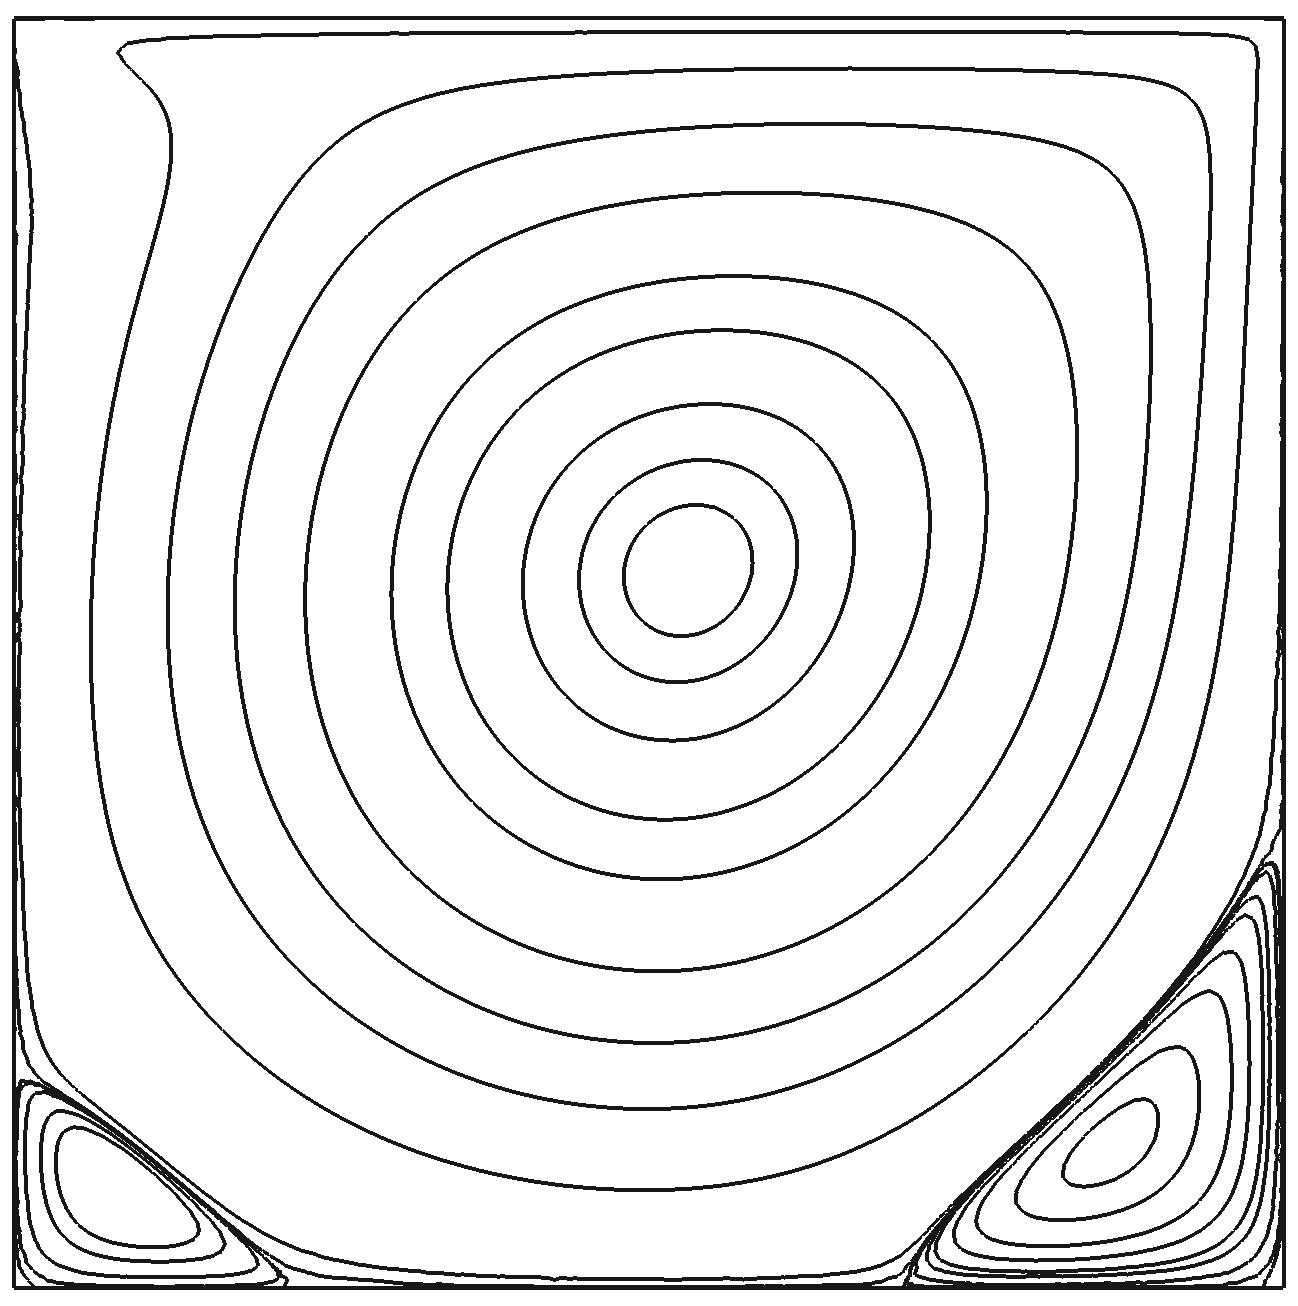
\includegraphics[width=7cm,clip]{examples_images/driven_cavity/driven_cavity_streamfunction.png}}
\subfigure{
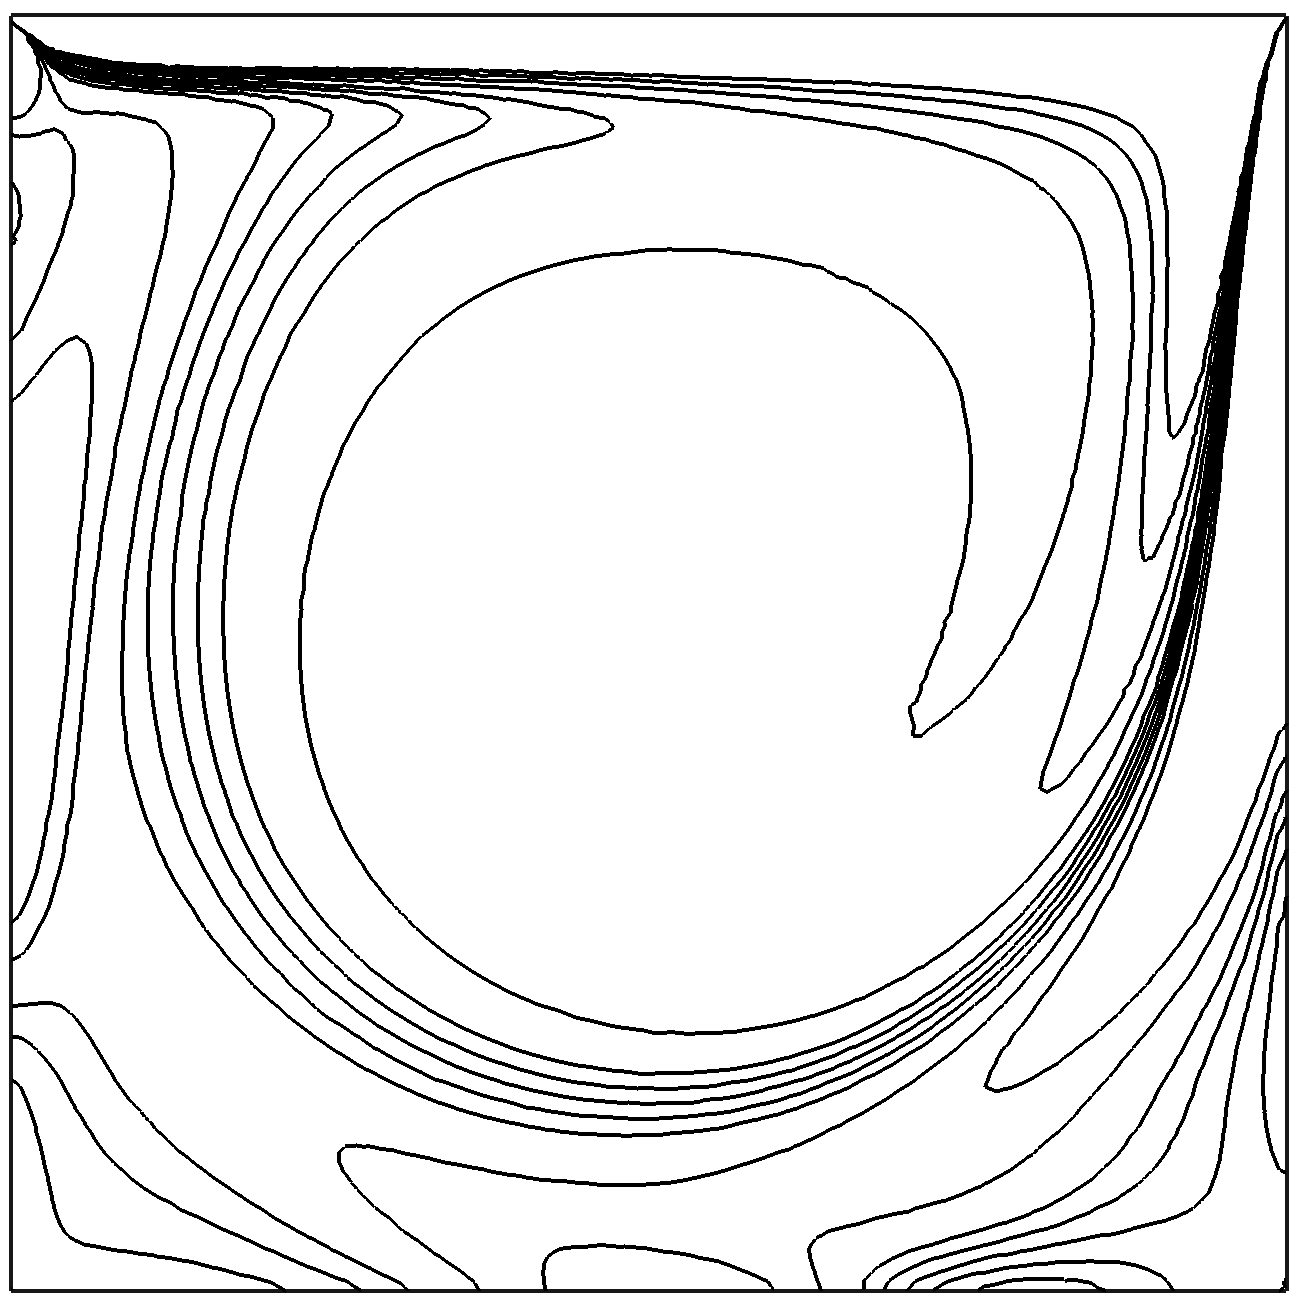
\includegraphics[width=7cm,clip]{examples_images/driven_cavity/driven_cavity_vorticity.png}}
\caption{Diagnostic fields from the lid-driven cavity problem at steady state at $1/128$ resolution.
Left: the streamfunction. Right: the vorticity. The contour levels are taken from those given by \cite{botella1998} in their tables
7 and 8.}
\label{fig:driven_cavity1}
\end{figure}


\subsection{Results}
Plots of the streamfunction and vorticity from the $h=1/128$ simulation are shown in figure \ref{fig:driven_cavity1}.
Observe the good qualitative agreement with \citep{botella1998,erturk2005,bruneau2006}. 
For a quantitative comparison we take advantage of the tabulated benchmark data available in these papers.
Only a subset of these are computed: the $u$ velocity at a series of points along the line $x=0.5$ and the
$v$ velocity at a series of points along the line $y=0.5$ from \citep{erturk2005}, the same quantities at
different points along the same lines as well as the pressure along both the $x=0.5$ and $y=0.5$ lines from 
\citep{botella1998}, and the kinetic energy and the minimum streamfunction value from \citep{bruneau2006}.
The RMS difference in the case of the first six sets of benchmark data are taken with values extracted from 
the numerical solution, and the absolute difference taken in the final two. These eight error values are
defined as error1, \ldots error8 respectively and and plotted for the four mesh resolutions in figure 
\ref{fig:driven_cavity2}.
Second order spatial convergence can clearly be seen.
Note that when reproducing these results, subtle changes to the mesh usually result in slight variations to the calculated errors and hence a different plot to that of figure~\ref{fig:driven_cavity2} will result. The order of convergence, however, should be the same.
Adaptive refinement is not particularly advantageous for the problem at this reasonably low Reynolds number, but
yields significant improvements in efficiency at higher Reynolds number where boundary layers and
recirculating eddies are more dynamic, anisotropic and smaller in size compared to the entire domain.

\begin{figure}
\centering
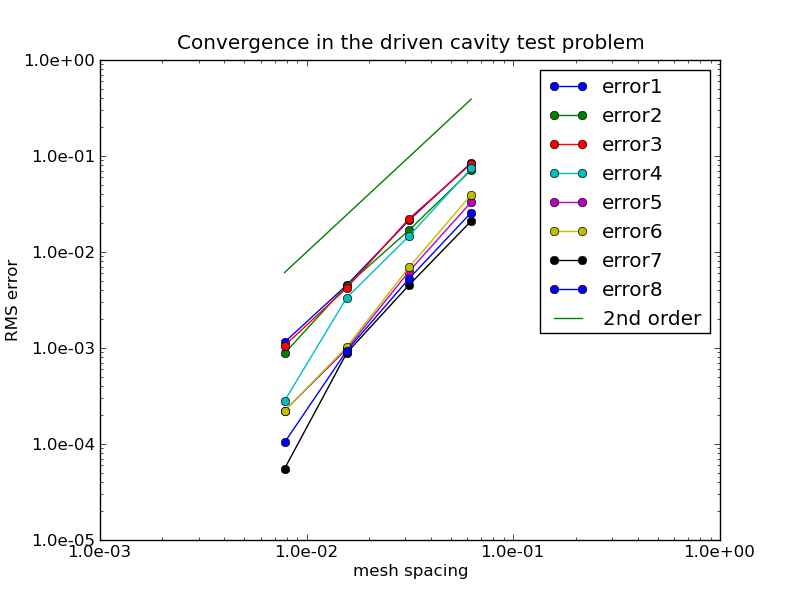
\includegraphics[width=10cm,clip]{examples_images/driven_cavity/driven_cavity_error_plot.png}
\caption{Convergence of the eight error metrics computed for the lid-driven cavity problem with mesh spacing. The eight
metrics are described in the text.}
\label{fig:driven_cavity2}
\end{figure}

\subsection{Exercises}
\begin{enumerate}
\item Examine the way that the $u=1$ lid condition is applied in the flml file. Why has it not been set as simply a constant?
Try changing it to a constant and see what happens to the errors that you achieve. [Hint: some people consider the "regularised" 
lid-driven cavity problem. Try finding some papers that discuss this, and update the boundary condition so it matches the 
regularised problem. Compare to benchmark data if you can find it].
\item The references given above include data from other Reynolds numbers. Try updating the problem set-up and the post-processing script which computes
the errors for a higher Reynolds number.
\item Try switching on mesh adaptivity, see section \ref{sec:using_mesh_adaptivity} (you will need to ensure that you have configured your \fluidity\ executable with \texttt{--enable-2d-adaptivity}). 
Test adapting based on different metrics, e.g. try weighting $u$, $v$ and $p$
differently and see what meshes you get. Try varying these weights as well as the maximum and minimum allowed element
sizes to see how they affect each other and the mesh that results. Can you get a metric that results in a lower
error for the same number of nodes compared to the fixed mesh (hint: it may be easier to achieve this at higher Reynolds numbers)?.
\item This example runs the lid-driven cavity problem with four different resolutions. On a 2.4GHz Intel machine, the runtime for the coarse resolution setup is below 15min, the next higher resolution takes about 30min, then 90min and finally about 350min for the highest resolution. To decrease the runtime for the high resolution case, try to run the it on 4 processors and check how much the runtime decreases.
\end{enumerate}


%%%%%%%%%%%%%%%%%%%%%%%%%%%%%%%%%%%%%%%%%%%%%%%%%%%%%%%%%%%%%%%%%%%
%---------------------2D BACKWARD FACING STEP------------------------%
%%%%%%%%%%%%%%%%%%%%%%%%%%%%%%%%%%%%%%%%%%%%%%%%%%%%%%%%%%%%%%%%%%%

\section{2D Backward facing step}
\label{sec:backward_facing_step_2d}


\subsection{Overview}
The backward-facing step is a classical CFD example and one of the most frequently selected
problems for simulating the separation and reattachment of turbulent flows.
It is also often used as a test problem for validating and benchmarking numerical codes.
At high Reynolds numbers and in three spatial dimensions the problem has substantial
computing requirements, making it an ideal HPC benchmark problem for use here.
In the context of ocean modelling flow separation is important
in large scale western boundary currents such as the Gulf Stream.

The problem has several important flow characteristics,
in particular the downstream length at which the flow reattaches with the bottom of the domain. 
The reattachment length is considered a sensitive measure of the quality of the numerical method.
It is used here to examine the impact of the k-epsilon turbulence model.

Results from \fluidity\ simulations at Reynolds number 132,000
are presented here. Numerical results using RANS from \cite{ilinca_97}
and experimental results from Kim \cite{ilinca_97} are used for comparison.

To run the example, use the commands \option{make preprocess TYPE=type}, \option{make run TYPE=type}
and \option{make postprocess TYPE=type}, where \option{type} is one of \option{reference} or
\option{kepsilon}. \option{reference} is on a fixed mesh with no turbulence model
or stabilisation. \option{kepsilon} uses the high-Re k-epsilon turbulence model (see \ref{sec:kepsilon})
on the same fixed mesh.

\subsection{Geometry}
A schematic of the domain is shown in figure \ref{Fig:Schematic2d}.
The expansion ratio is 3:2, consistent with \cite{ilinca_97}.

\begin{figure}
\centering
\pdffig[width=17.0cm]{examples_images/backward_facing_step/backward_facing_step_2d-mesh}
\caption{Schematic of the domain for the two-dimensional flow past a backward facing step.}
\label{Fig:Schematic2d}
\end{figure}

\subsection{Initial and boundary conditions}
The inlet velocity profile is a log profile extending reflected in the midpoint of the inlet. Below a small distance $z_0=0.1$ from the top and bottom of the inlet, the velocity is 0.
\begin{equation*}
u(z) =
  \begin{cases}
    0.0 & \text{if } z \leq 1+z_0 \\
    \log \left(\frac{z-1}{z_0}\right) & \text{if } 1+z_0 < z \leq 2.0 \\
    \log \left(\frac{3.0-z}{z_0}\right) & \text{if } 2.0 < z \leq (3.0-z_0) \\
    0.0 & \text{if } 3.0-z_0 < z
  \end{cases}
\end{equation*}

The log law of the wall is applied weakly on the upper and lower boundaries.
This approach has been found useful in high-Reynolds number flow, allowing coarser near-wall mesh resolution.

\subsection{Results}
Three snapshots of the velocity magnitude from the k-epsilon run at $Re=132000$
are shown in figure \ref{Fig:velo-magnitude-2d} at 3 times during the flow's evolution to steady-state.

Vertical profiles of $\vec{u}$ at several points downstream of the step are shown
in figure \ref{Fig:UProfiles2d}. The evolution of the flow to the converged solution can be seen.
The evolution of the reattachment length is shown in figure \ref{Fig:RL2d}.

The reattachment length was defined here to be the length (normalised by step height $h=1$)
from the step at which the zero-contour of the $x$-component of $\vec{u}$ intersects with
the bottom boundary. This quantity was computed from $\vec{u}$
using the VTK library. For the simulation described, the reattachment
length converged to approximately 9.1 times the step height,
whereas the RANS simulation of \cite{ilinca_97} reattaches at 6.2 and Kim's experiment at 7.0.
The discrepancy may be due to the difference in discretisation or solution procedure from Ilinca.

\begin{figure}
\centering
\subfigure{\pdffig[width=15.0cm]{examples_images/backward_facing_step/velo-magnitude-2d-5sec}}
\subfigure{\pdffig[width=15.0cm]{examples_images/backward_facing_step/velo-magnitude-2d-10sec}}
\subfigure{\pdffig[width=15.0cm]{examples_images/backward_facing_step/velo-magnitude-2d-50sec}}
\caption{Snapshots of the velocity magnitude from the 2D run at times 5, 10 and 50 time units
(top to bottom) from the k-epsilon run.
The evolution of the dynamics to steady state can be seen, in particular the downstream movement
of the streamline reattachment point (where zero-magnitude contour touches bottom).}
\label{Fig:velo-magnitude-2d}
\end{figure}

\begin{figure}
\centering
\pdffig[width=17.0cm]{examples_images/backward_facing_step/velocity_profiles_kim_kepsilon}
\caption{Streamwise velocity profiles from the 2D run at $x/h=1.33, 2.66, 5.33, 8.0 \text{ and } 16.0$
downstream of the step, where $h=1$ is the step height. The converged solution is in blue.
Ilinca's numerical and Kim's experimental data \citep{ilinca_97} are in red and black respectively.
The recirculation region is indicated by negative velocities.}
\label{Fig:UProfiles2d}
\end{figure}

\begin{figure}
\centering
\pdffig[width=13.0cm]{examples_images/backward_facing_step/reattachment_length_kim_kepsilon}
\caption{Evolution of reattachment length in k-epsilon simulation.}
\label{Fig:RL2d}
\end{figure}

The solution for the k-epsilon run also contains information on the turbulent kinetic energy, turbulent dissipation and eddy viscosity, which can be plotted in Mayavi or Paraview.

%%%%%%%%%%%%%%%%%%%%%%%%%%%%%%%%%%%%%%%%%%%%%%%%%%%%%%%%%%%%%%%%%%%
%---------------------3D BACKWARD FACING STEP---------------------%
%%%%%%%%%%%%%%%%%%%%%%%%%%%%%%%%%%%%%%%%%%%%%%%%%%%%%%%%%%%%%%%%%%%

\section{3D Backward facing step}
\label{sec:backward_facing_step_3d}

\subsection{Configuration}
Please note, this 3D example is intended to be run in parallel (see \ref{decomp_meshes_parallel}),
because it requires relatively fine mesh to resolve the eddies behind the step.
More information on running \fluidity\ in parallel is found in \ref{sec:running_fluidity_in_parallel}.

The example is run in a very similar way to the other examples.
To run in serial, the example is run in exactly the same way to the other examples, using
the commands \option{make preprocess}, \option{make run} and \option{make postprocess}.
To run in parallel with your chosen number of processors (\option{np}), using the command
\option{make preprocess NPROCS=np} creates a mesh and decomposes it into (\option{np}) parts, and
the command \option{make run NPROCS=np} runs \fluidity\ as (\option{np}) processes on (\option{np}) processors.
The command \option{make postprocess NPROCS=np} runs the parallel-specific data processing script.

The Reynolds number of this example is set deliberately low (Re=155) in order to
allow convergence to a steady state, and demonstrate the reduction in runtime obtained
by running in parallel.

\subsection{Geometry}
A schematic of the domain is shown in figure \ref{Fig:Schematic3d}.
A logarithmic velocity profile is imposed at the left hand boundary (inflow).
The region directly downstream of the step is of interest in this problem.

\begin{figure}
\centering
\pdffig[width=12.0cm]{examples_images/backward_facing_step/backward_facing_step_3d-schematic}
\caption{Schematic of the domain for the three-dimensional flow past a backward facing step
problem.}
\label{Fig:Schematic3d}
\end{figure}

Following \cite{le1997} the dimensions are: $L_x=30$, $L_i=10$, $L_y=4$, $h=1$, $L_z=6$,
so that $L_z-h=5$ and the expansion ratio is $L_z/(L_z-h)=1.2$.
The base of the domain is located at $z=0$, the inflow plane is given by $x=-10$ with the step
at $x=0$, and the back of the domain in the spanwise direction is given by $y=0$.

\subsection{Initial and boundary conditions}
The inflow boundary condition at $x=-10$ is a log profile given by
\begin{equation*}
u(z) =
  \begin{cases}
    0.0 & \text{if } z-h \leq z_0 \\
    \frac{u_{\tau}}{\kappa} \log \left(\frac{z - h}{z_0}\right) & \text{if } z_0 < z-h
  \end{cases}
\end{equation*}

with parameters $u_{\tau} = 0.1$, $z_0 = 0.01$ and $\kappa = 0.41$.

No-normal flow, free-stress boundary conditions are applied at the upper and lateral
(spanwise) boundaries:
\begin{eqnarray*}
&&w=0,\quad \frac{\partial u}{\partial z} = \frac{\partial v}{\partial z} = 0 \quad\textrm{--- upper boundary},\\
&&v=0,\quad \frac{\partial u}{\partial z} = \frac{\partial w}{\partial z} = 0 \quad\textrm{--- lateral boundaries}.
\end{eqnarray*}

Free-stress boundary conditions are applied at the outflow boundary boundary:
\begin{equation*}
\frac{\partial u}{\partial x} = \frac{\partial v}{\partial x} = \frac{\partial w}{\partial x} = 0.
\end{equation*}

No-slip boundary conditions are applied at the bottom of the domain and at the step down:
\begin{equation*}
u=v=w=0.
\end{equation*}

\subsection{Results}
Three snapshots of the velocity vectors are shown in figure \ref{Fig:velo-magnitude-3d}
at times 5, 10 and 50 seconds.
Vertical profiles of $\vec{u}$ at several points downstream of the step are shown in figure
\ref{Fig:UProfiles3d}, in which the velocity data has been averaged across the span of the domain
to obtain quasi-2D data. The reattachment point is clearly between $x/h=6$ and $x/h=10$.
In fact the flow reattaches at $x/h \approx $.

The postprocessing script plots graphs of the reattachment length
and velocity profiles, which are compared against the DNS data from \cite{le1997}.

\begin{figure}
\centering
\subfigure{\pdffig[width=15.0cm]{examples_images/backward_facing_step/velo-magnitude-3d-5sec}}
\subfigure{\pdffig[width=15.0cm]{examples_images/backward_facing_step/velo-magnitude-3d-10sec}}
\subfigure{\pdffig[width=15.0cm]{examples_images/backward_facing_step/velo-magnitude-3d-50sec}}
\caption{From top to bottom: vertical plane cuts through the 3D domain showing
the velocity magnitude at times 5, 25 and 50 time units.
The evolution of the dynamics to steady state can be seen, in particular the downstream movement
of the streamline reattachment point (indicated by contours of $U=0$).}
\label{Fig:velo-magnitude-3d}
\end{figure}

\begin{figure}
\centering
\pdffig[width=17.0cm]{examples_images/backward_facing_step/velo_profiles_3d}
\caption{Streamwise velocity profiles from the 3d run at $x/h=4, 6, 10 \text{ and } 19$
downstream of the step, where $h=1$ is the step height, at $t=5$ seconds.}
\label{Fig:UProfiles3d}
\end{figure}

A more rigorous analysis would involve repeating the experiment for a range of
Reynolds numbers and comparing the reattachment length of multiple model runs.
The Reynolds number in this example is considerably lower than the DNS, 
in order to reduce simulation run time and suppress turbulent eddies, which
results in the differences seen. To get closer to the DNS, try reducing the
viscosity from $1.0e-2$ (Re=155) to $3.04e-4$ (Re=5100).

%%%%%%%%%%%%%%%%%%%%%%%%%%%%% %%%%%%%%%%%%%%%%%%%%%%%%%%%%%%%%%%%%%
%----------------------Sphere------------------------------------%
%%%%%%%%%%%%%%%%%%%%%%%%%%%%%%%%%%%%%%%%%%%%%%%%%%%%%%%%%%%%%%%%%%%

\section{Flow past a sphere: drag calculation}
\label{sec:flow_past_sphere}
\subsection{Overview}
In this validation test uniform flow past an isolated sphere is simulated
and the drag on the sphere is calculated and compared to a curve optimised
to fit a large amount of experimental data.

\subsection{Configuration}
The sphere is of unit diameter centred at the origin. The entire domain is
the cuboid defined by $-10\le x\le 20$, $-10\le y\le 10$, $-10\le z\le 10$.
GiD is used to mesh the initial geometry.

The unsteady momentum equations with nonlinear advection and viscous terms
along with the incompressibility constraint are solved. Free slip velocity
boundary conditions are applied at the four lateral boundaries, $u=1$, $v=w=0$ is
applied at the inflow boundary $x=-10$, and a free stress boundary condition
applied to the outflow at $x=20$. 

A series of Reynolds numbers in the range
$Re\in [1,1000]$ are considered. The problem is run for a long enough
period that the low Reynolds number simulations reach steady state, and the
higher Reynolds number runs long enough that a wake develops behind the
sphere and boundary layers on the sphere are formed.  This is deemed
sufficient for the purposes of this test; the example is to demonstrate
how such a problem would be set up, not conduct an in-depth 
investigation of the physics of this problem.

Here an unstructured
tetrahedral mesh is used along with mesh adaptivity. 
Figure \ref{fig:flow_past_sphere_2} shows a snapshot of the
mesh and velocity vectors taken from a Reynolds number 1000 simulation. The
mesh can be seen to be resolving the wake and the boundary layers on the
sphere with enhanced anisotropic resolution. At higher Reynolds numbers the
dynamics become more complex and if a full numerical study was being
conducted here more care would be taken in the choice of mesh optimisation
parameters and the use of averaged values from simulations allowed to run
for longer periods. The drag coefficient is calculated from
\begin{equation}
C_D = \frac{F_x}{\frac{1}{2}\rho u_0^2 A},\qquad F_x = \int_S (n_xp - n_i\tau_{ix})\;dS,
\label{eqn:drag_coeff}
\end{equation}
where $\rho$ is the density, taken here to be unity; 
$u_0$ is the inflow velocity, here unity; 
and $A$ is the cross-sectional area of the sphere, here $\pi^2/4$. 
$F_x$ is the force 
exerted on the sphere in the free stream direction;
$S$ signifies the surface of the sphere; $n$ is the 
unit outward pointing normal to the sphere 
($n_x$ is the $x$-component and $n_i$ the $i^{\textrm{th}}$ 
component, here summation over repeated indices is assumed); 
$p$ is the pressure and $\tau$ is the stress tensor;
see \citet{panton2006}.

\begin{figure}
\centering
\subfigure{
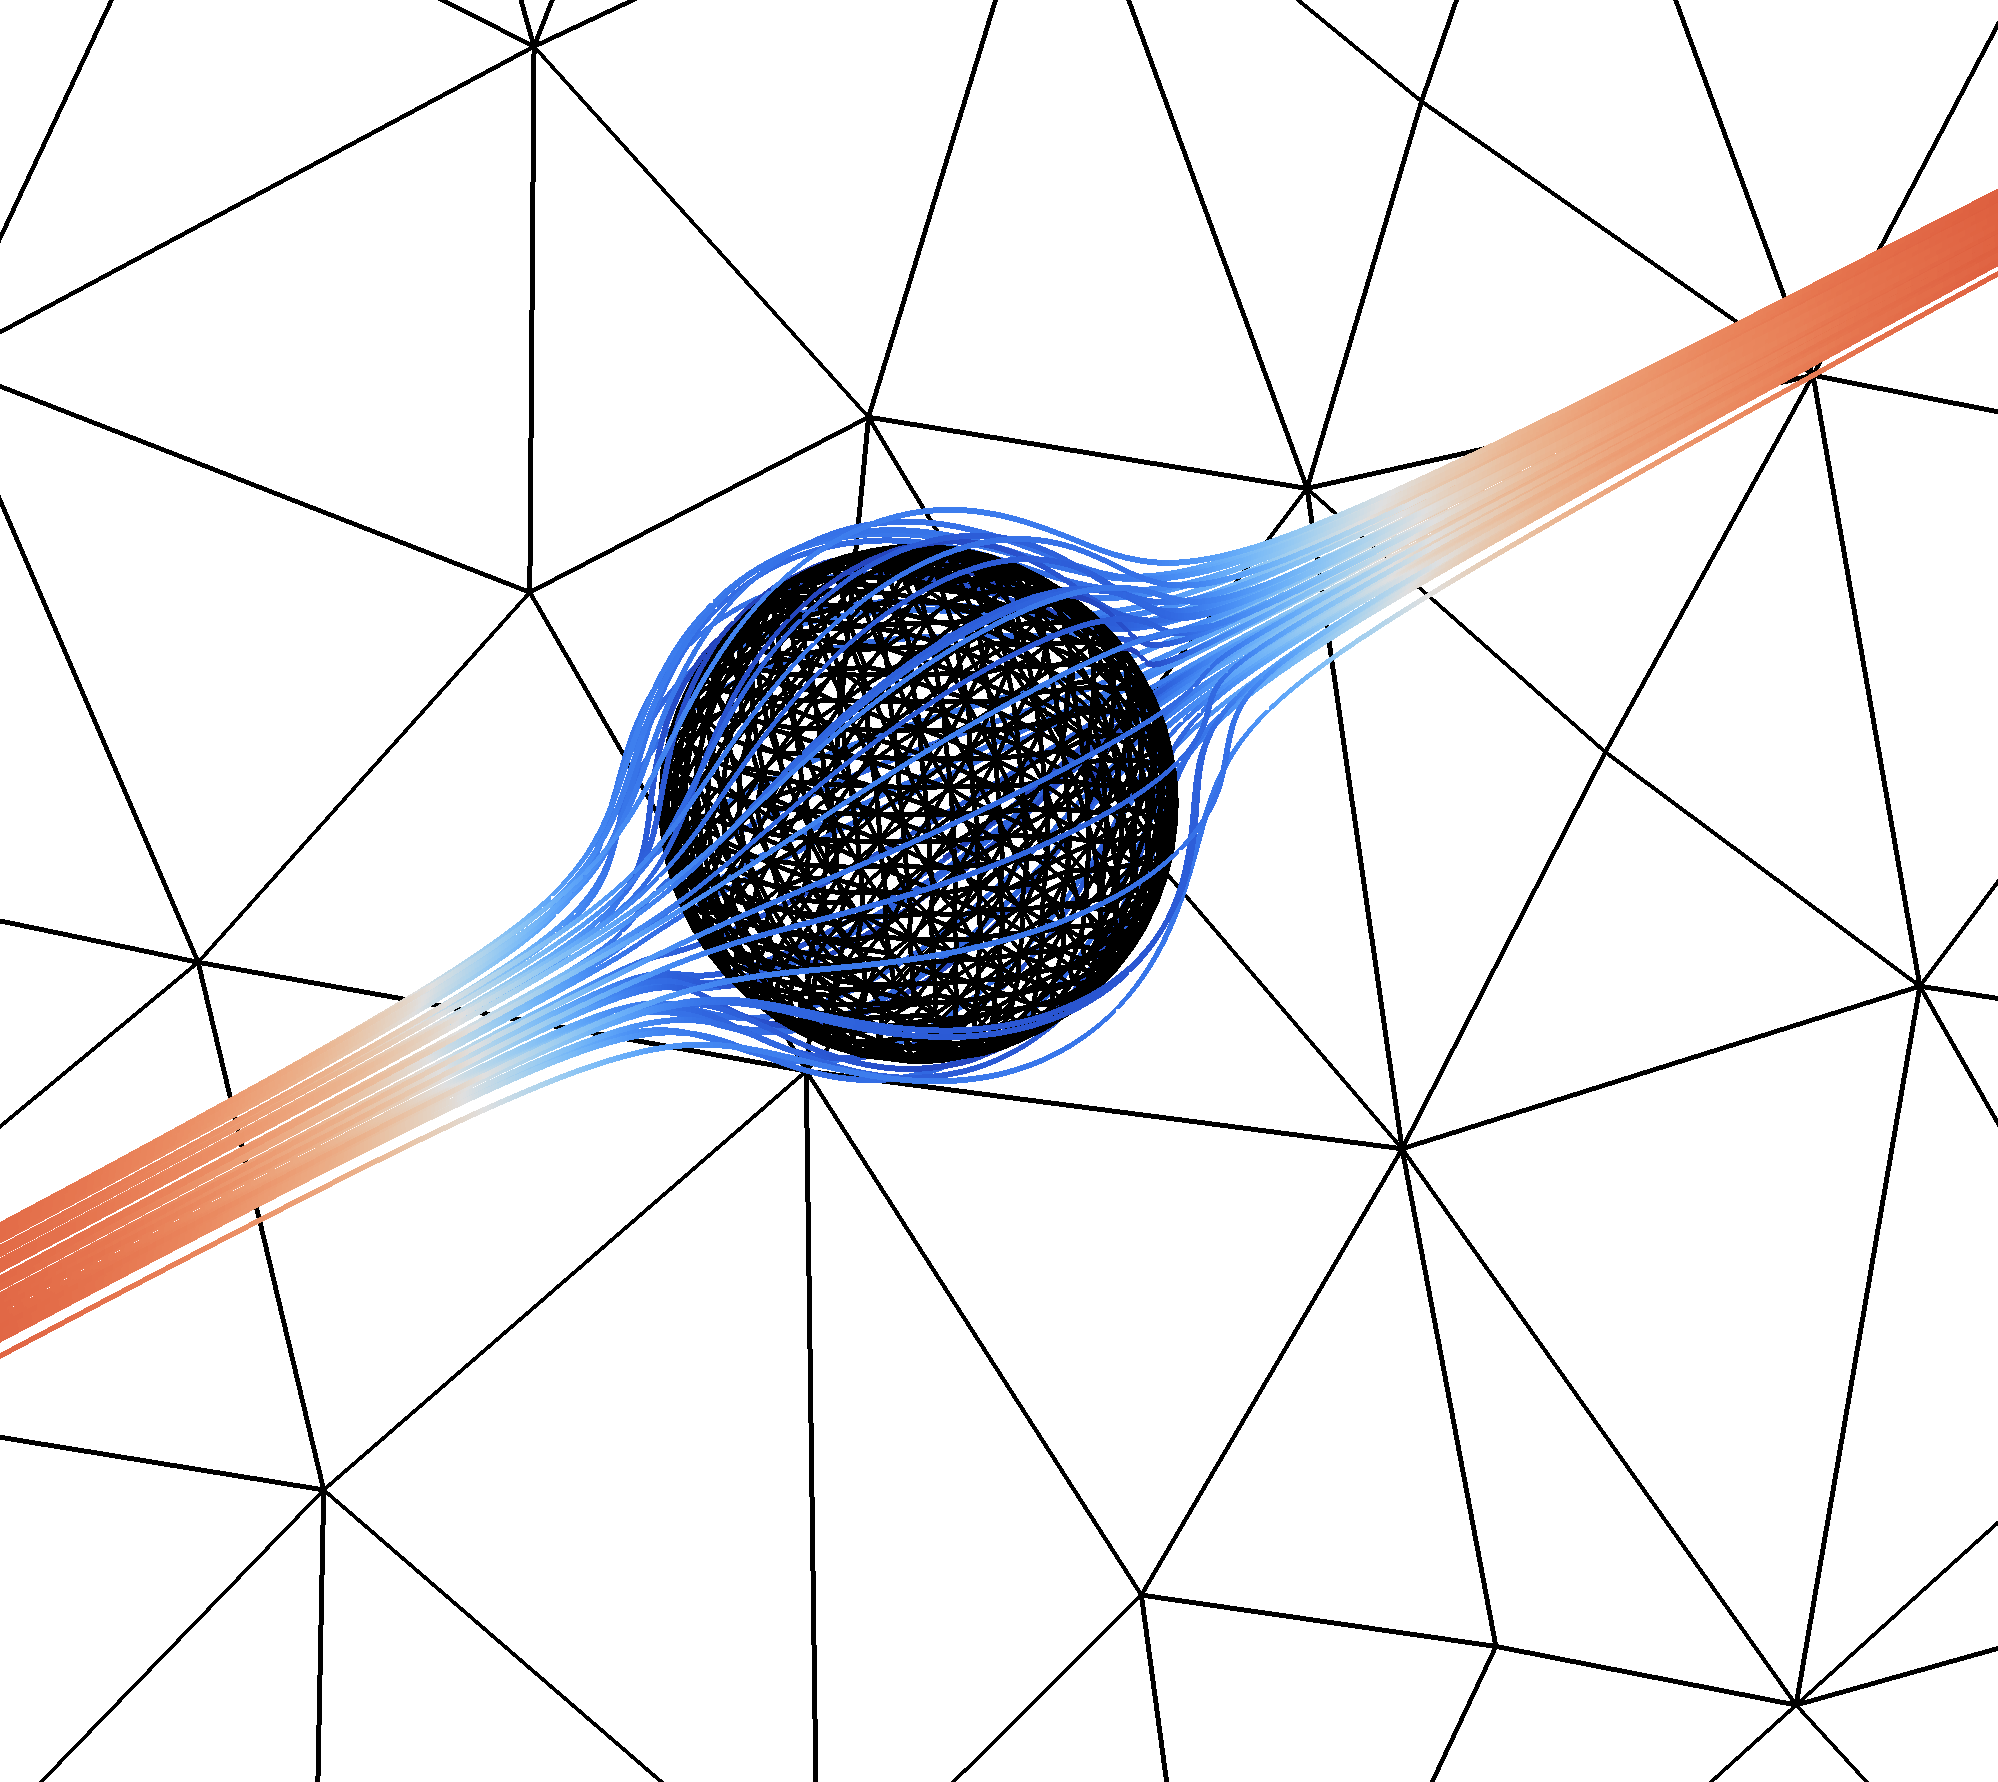
\includegraphics[width=6cm,clip]{examples_images/flow_past_sphere/sphere-Re1-streamlines.png}}
\subfigure{
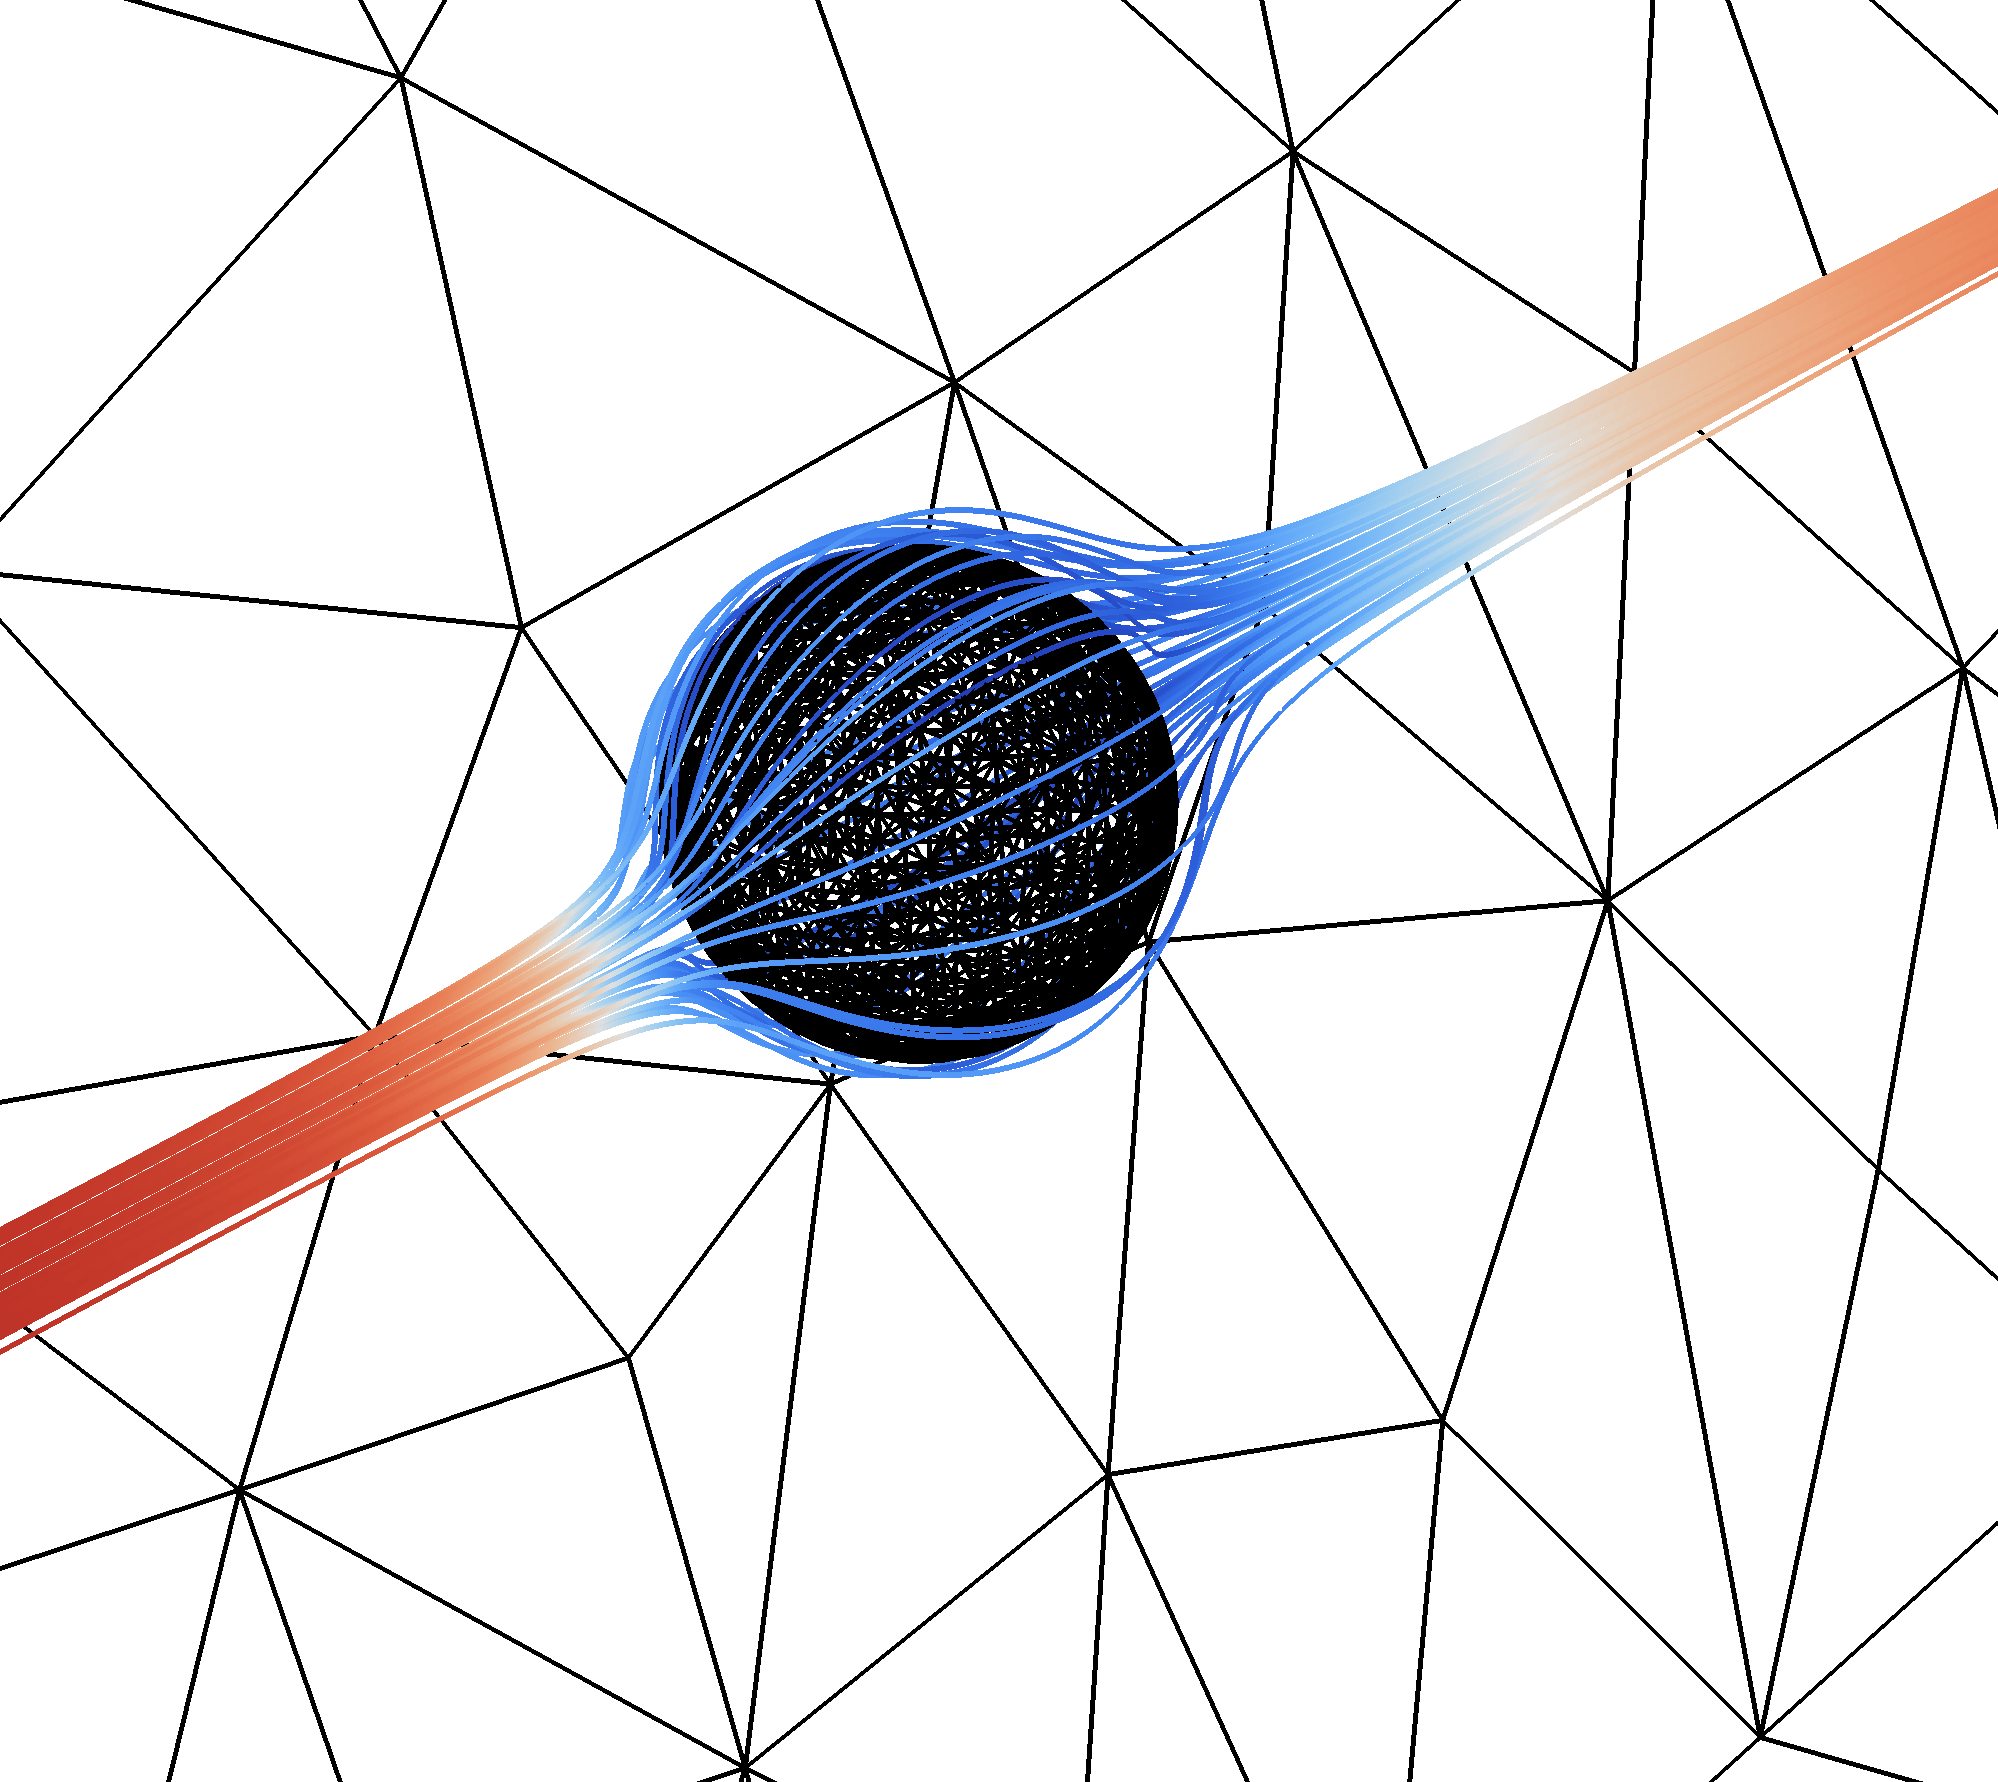
\includegraphics[width=6cm,clip]{examples_images/flow_past_sphere/sphere-Re10-streamlines.png}}
\subfigure{
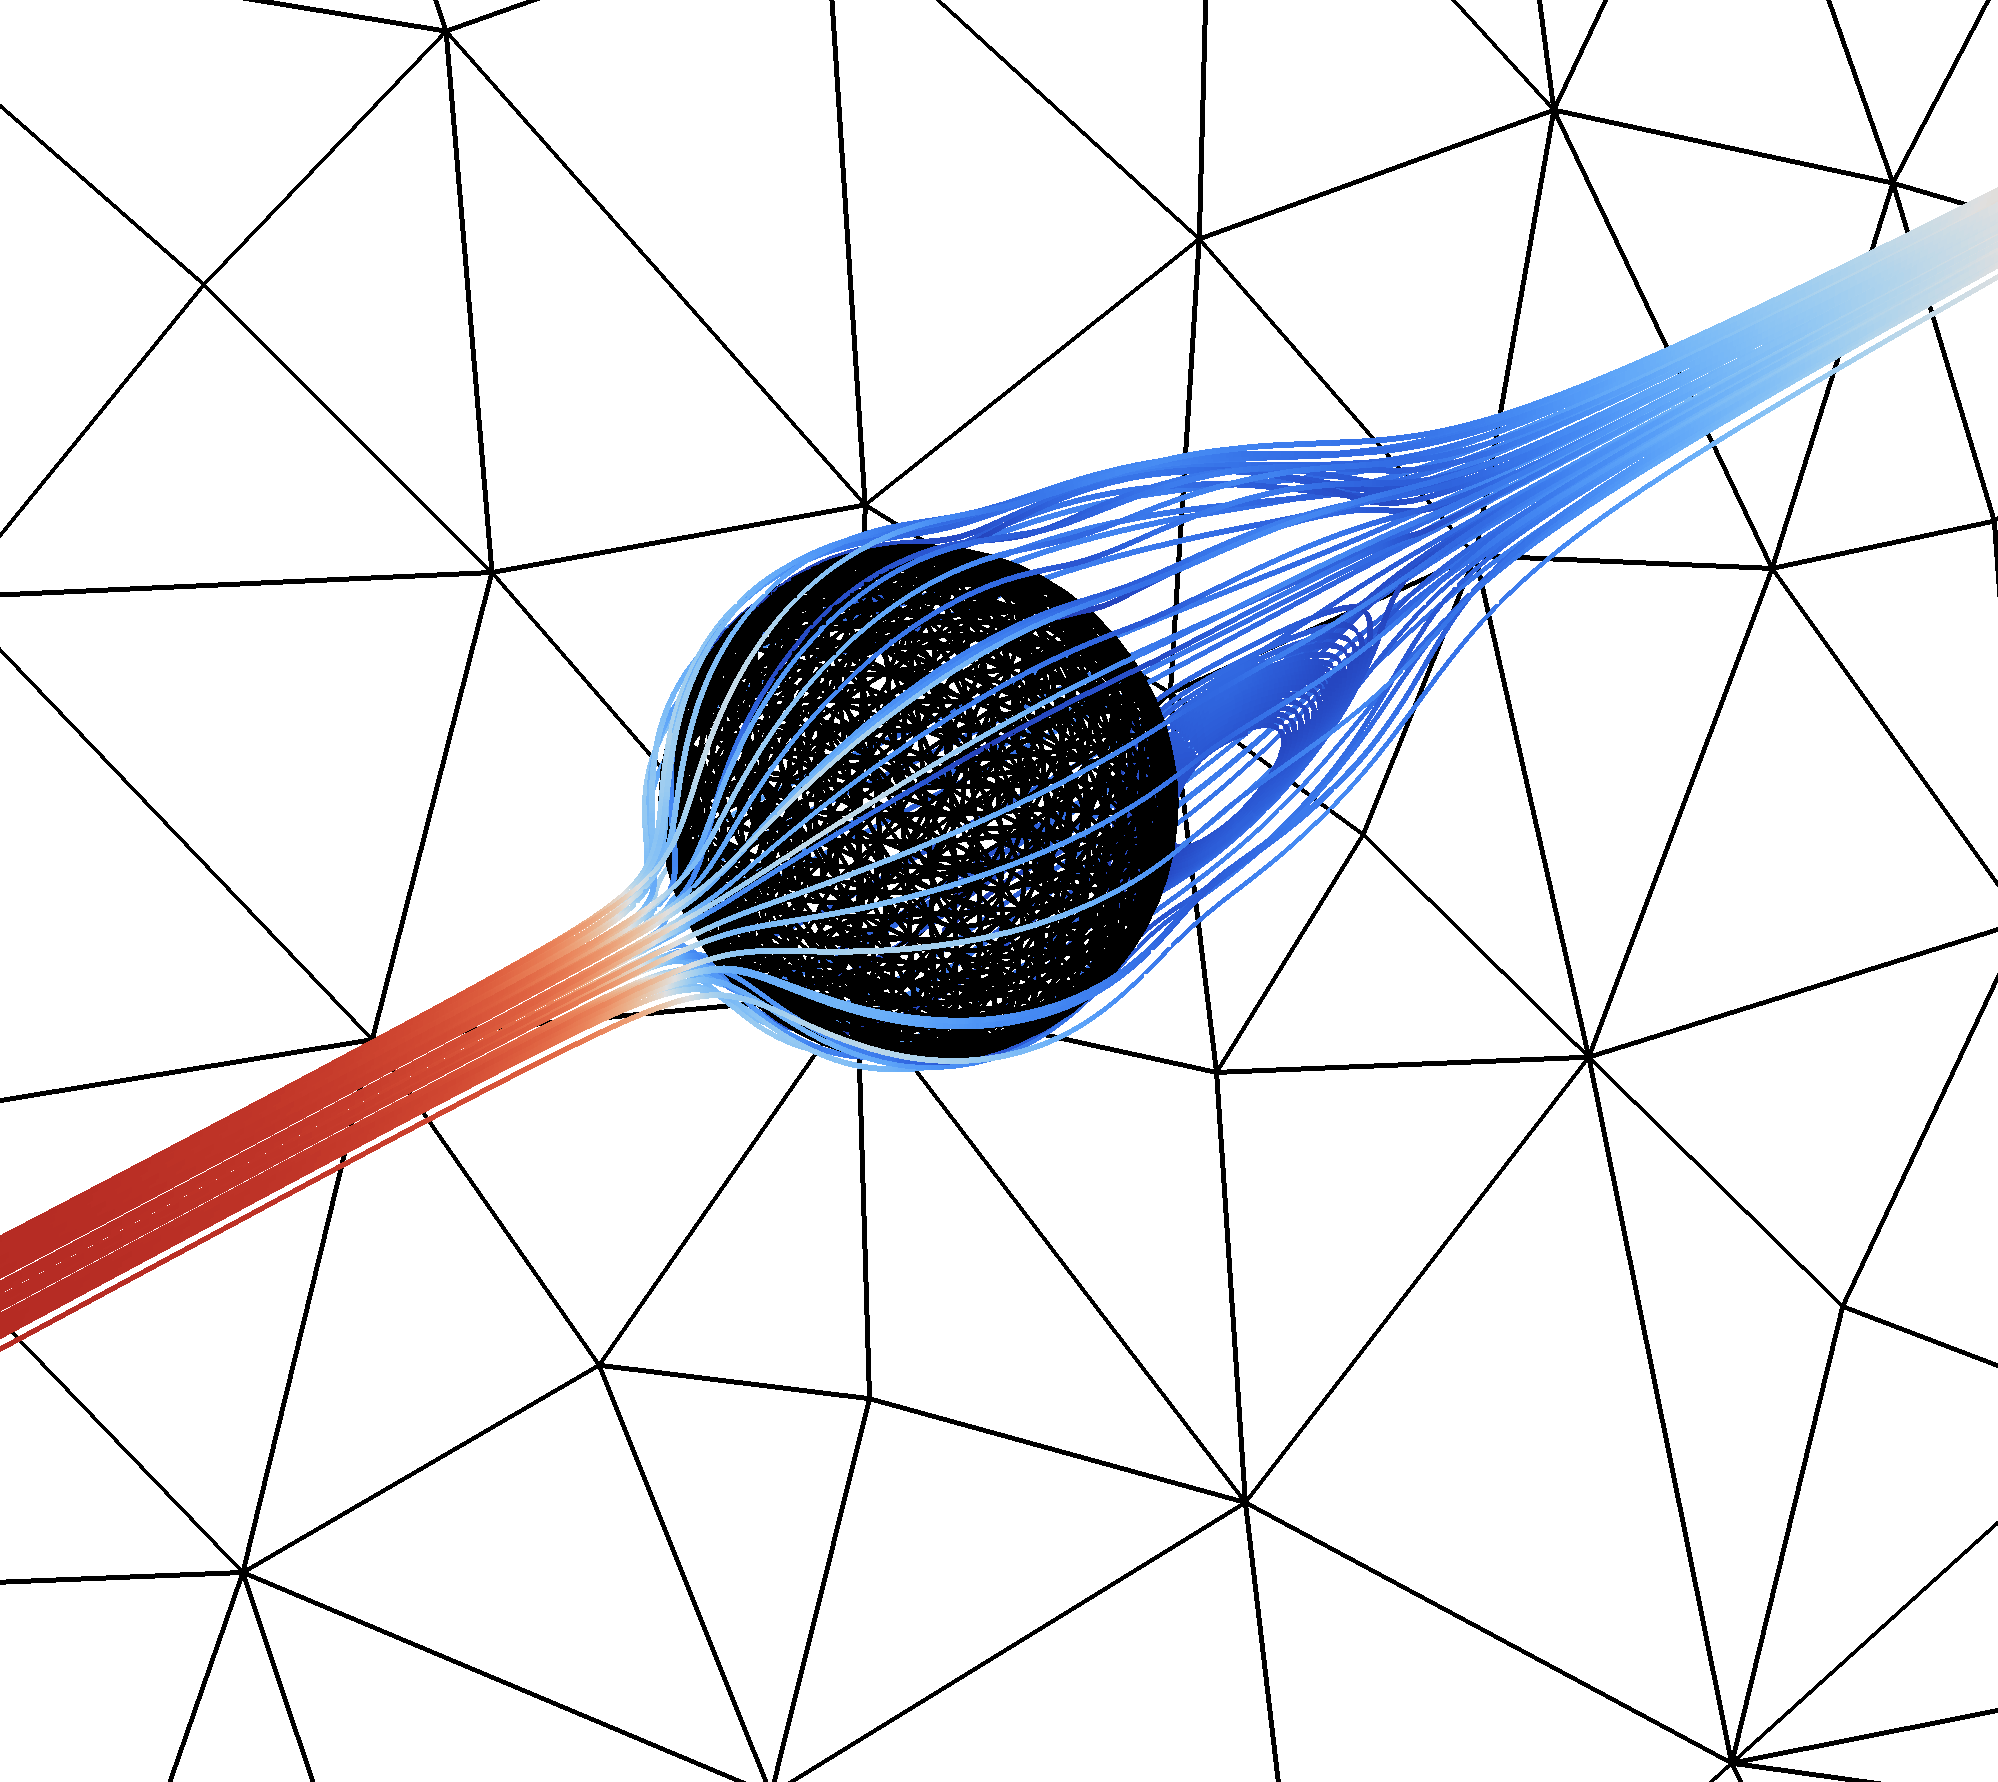
\includegraphics[width=6cm,clip]{examples_images/flow_past_sphere/sphere-Re100-streamlines.png}}
\subfigure{
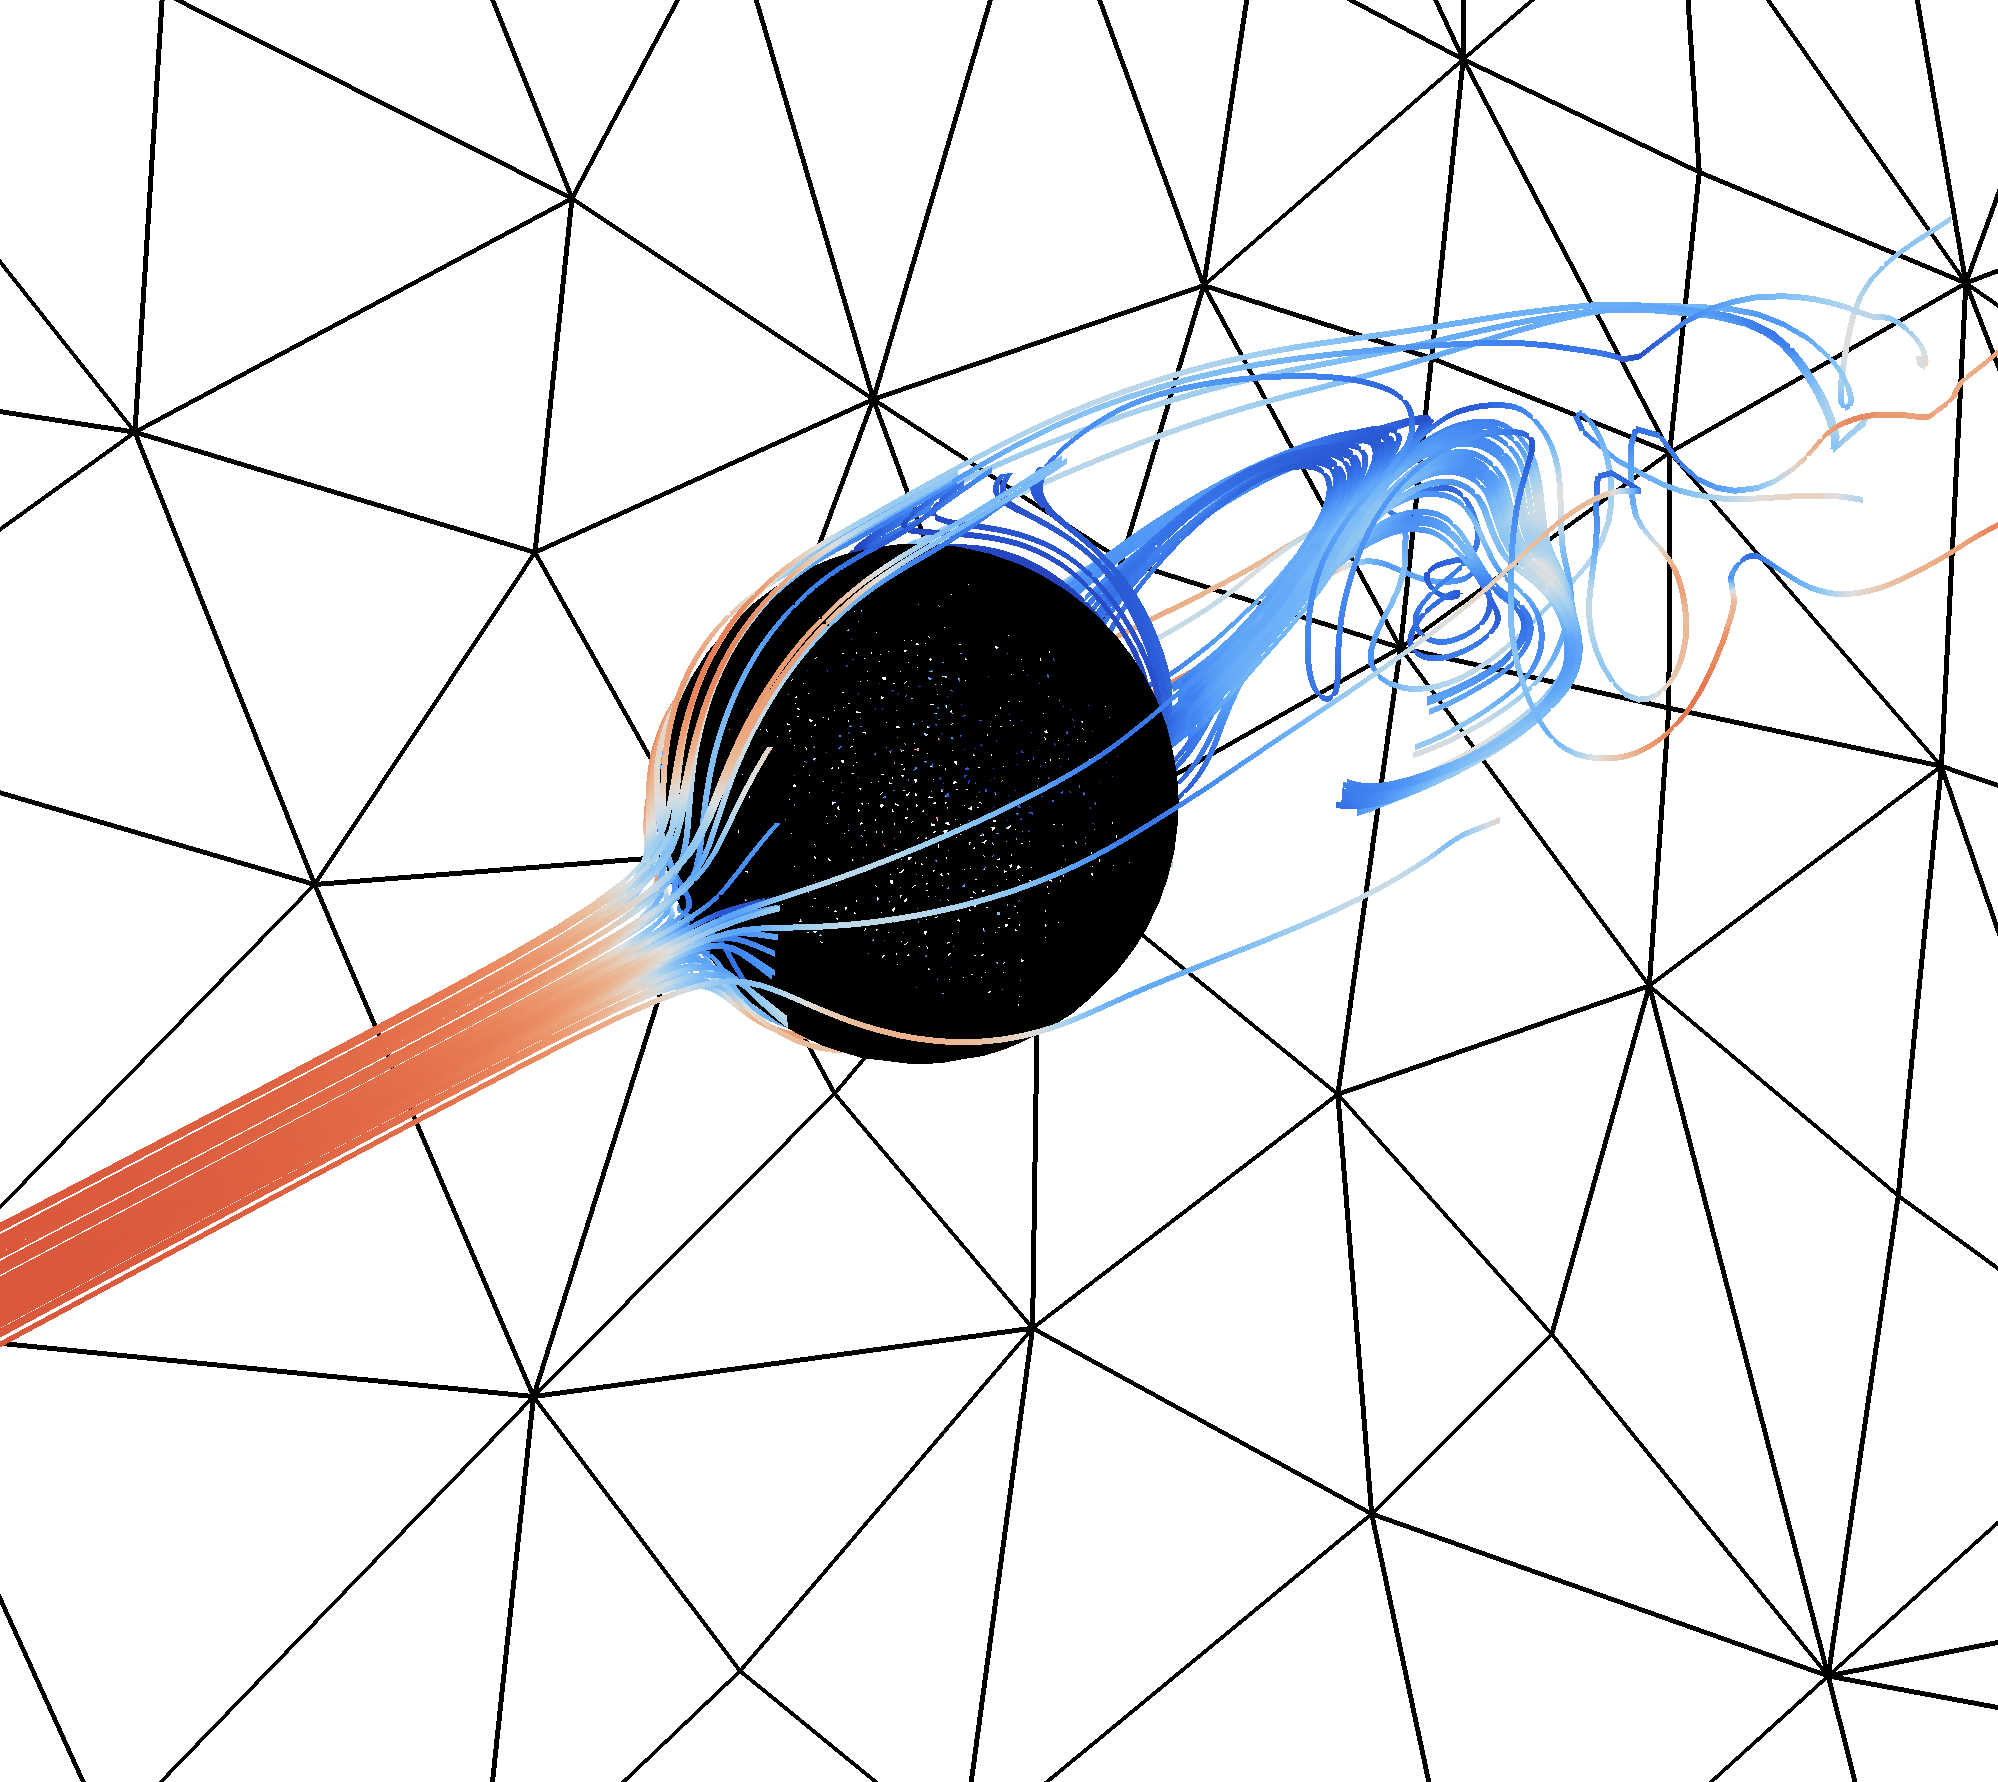
\includegraphics[width=6cm,clip]{examples_images/flow_past_sphere/sphere-Re1000-streamlines.png}}
\caption{Streamlines and surface mesh in the flow past the sphere example. Top-left to bottom-right
show results from Reynolds numbers $Re=1,10,100,1000$.}
\label{fig:flow_past_sphere_1}
\end{figure}


\begin{figure}
\centering
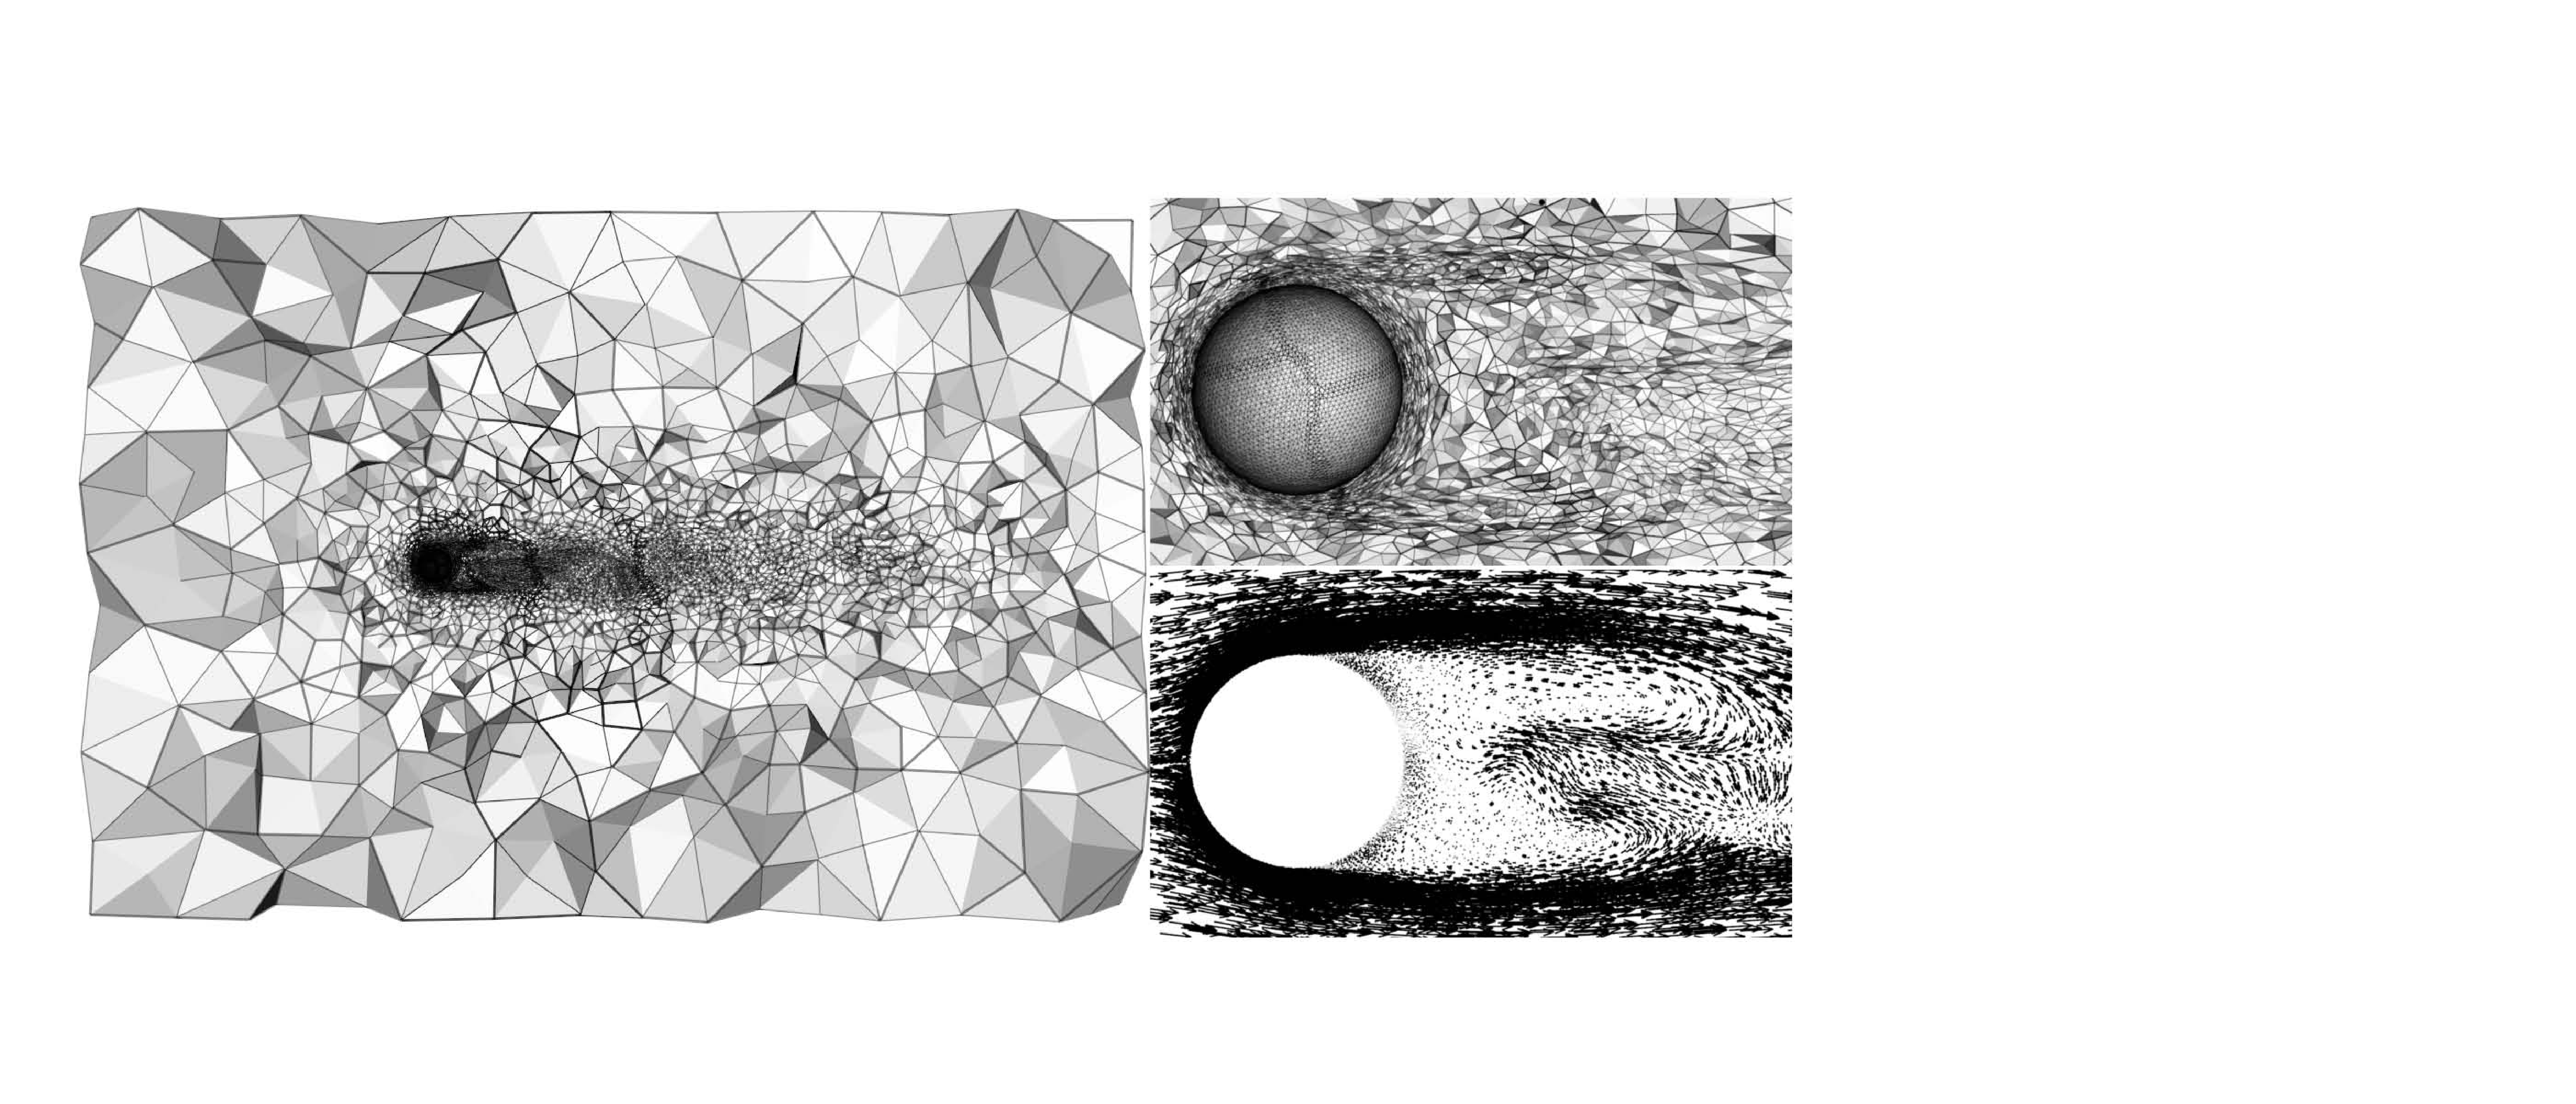
\includegraphics[width=15cm,clip]{examples_images/flow_past_sphere/sphere-Re1000-combined.pdf}
\caption{Details of the mesh and flow at $Re=1000$.}
\label{fig:flow_past_sphere_2}
\end{figure}

\subsection{Results}
Figure \ref{fig:flow_past_sphere_1} shows streamlines close to the sphere and the surface mesh.
The mesh can be seen to be much finer on the sphere compared to the far wall seen in the background.
This is emphasised in figure \ref{fig:flow_past_sphere_2} where a more detailed plot of the mesh (with
half of the domain removed) over the whole domain and close to the sphere, and the velocity vectors
close to the sphere are shown.

Figure \ref{fig:flow_past_sphere_3} shows a comparison between the computed drag coefficient with
a correlation (to a large amount of laboratory data) taken from \citet{brown2003}:
\begin{equation}
C_D = \frac{24}{Re}\left(1+0.15Re^{0.681}\right) + \frac{0.407}{1+\frac{8710}{Re}}.
\label{eqn:sphere_drag_corr}
\end{equation}
Excellent agreement can be seen at the range of Reynolds numbers tested in this exercise.


\begin{figure}
\centering
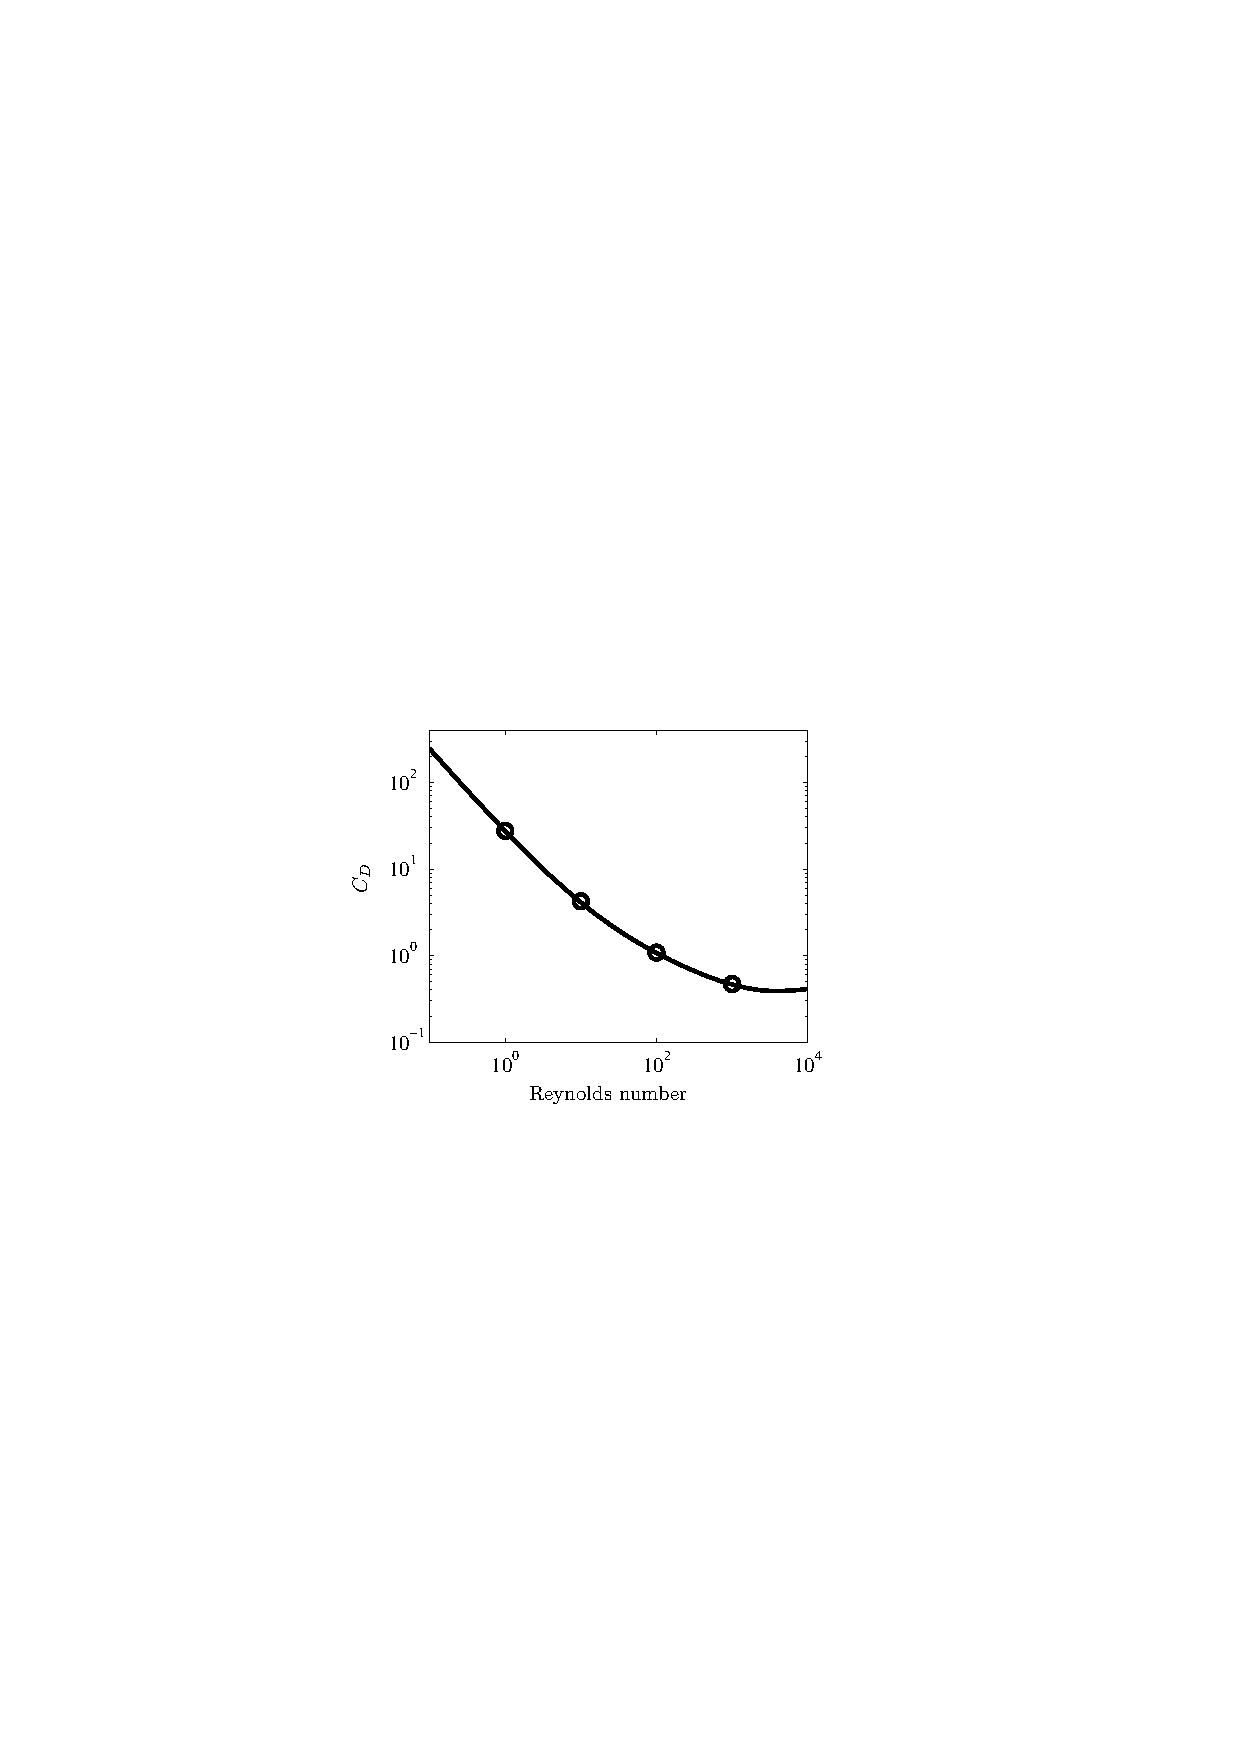
\includegraphics[width=8cm,clip]{examples_images/flow_past_sphere/Sphere_Drag.pdf}
\caption{Comparison between the numerically calculated drag coefficients ($C_D$, circles) and the correlation \eqref{eqn:sphere_drag_corr} (solid line)
for $Re=1,10,100,1000$.}
\label{fig:flow_past_sphere_3}
\end{figure}



\subsection{Exercises}
\begin{enumerate}
\item We actually compute the (vector) force on the sphere and output this to the stat file. This can then be converted to the drag coefficient 
via \eqref{eqn:drag_coeff}. Write a Python function to do this conversion and the error from the correlation \eqref{eqn:sphere_drag_corr}.
\item Try varying some of the discretisation and adaptivity parameters to see what the impact on the accuracy of the
calculated drag is.
\item Try changing the shape of the object, e.g. benchmark data is also available for flow past a cylinder \citep{schafer1996}.
\end{enumerate}


%%%%%%%%%%%%%%%%%%%%%%%%%%%%% %%%%%%%%%%%%%%%%%%%%%%%%%%%%%%%%%%%%%
%----------------------CHANNEL------------------------------------%
%%%%%%%%%%%%%%%%%%%%%%%%%%%%%%%%%%%%%%%%%%%%%%%%%%%%%%%%%%%%%%%%%%%

\section{Rotating periodic channel}
\label{sec:periodic_channel}

\subsection{Overview}

This problem provides a convergence test for the \PoDGPt\ element pair.
Utilising almost all the terms of the incompressible Navier-Stokes equations
in two dimensions.

The domain is a unit square which is periodic in the zonal direction. The
North and South boundaries are zero slip (i.e. $\vec{u}=0$). The remaining
parameters are as follows:

\begin{tabular}{lll}
  Coriolis parameter & $f$ & $1$ \\
  Viscosity & $\nu$ & $1$ 
\end{tabular}

The flow is driven by a velocity source term:
\begin{equation}
  \vec{F}=
  \begin{bmatrix}
    y^3 \\
    0
  \end{bmatrix}
\end{equation}

So the whole system of equations becomes:
\begin{gather}
  \ppt{u}+u\ppt[x]{u}-v=-\grad p + \grad^2 u +y^3\\
  \ppt{v}+v\ppt[y]{v}+u=-\grad p + \grad^2 v\\
  \div\vec{u}=0
\end{gather}

This system has a steady solution at:
\begin{gather}
  \vec{u}=
  \begin{bmatrix}
    \frac{1}{20}(y-y^5)\\
    0
  \end{bmatrix}\\
  p=\frac{1}{120}y^6-\frac{1}{40}y^2+C
\end{gather}
Where $C$ is an arbitrary constant resulting from the use of Dirichlet
boundary conditions on both the domain boundaries.

\subsection{Results}

Since the maximum velocity in the domain is approximately 0.025, the
Reynolds number for this solution is much smaller than 1 so the flow is
safely within the laminar regime and will remain steady. Figure
\ref{fig:periodic_channel}\ shows the forcing term for velocity and the
analytic solutions for velocity and pressure.


\begin{figure}[htbp]
  \centering
  \onlypdf{\begin{pdfdisplay}}
    \psfrag{u source}{$\vec{u}$ source}
    \psfrag{u solution}{$\vec{u}$ solution}
    \psfrag{p solution}{$p$ solution}
    \psfrag{0}{0}
    \psfrag{0.2}{0.2}
    \psfrag{0.4}{0.4}
    \psfrag{0.5}{0.5}
    \psfrag{0.2}{0.6}
    \psfrag{0.8}{0.8}
    \psfrag{1}{1}
    \psfrag{y}{$y$}
    \psfrag{-0.01}{-0.01}
    \psfrag{-0.02}{-0.02}
    \psfrag{0.01}{0.01}
    \psfrag{0.02}{0.02}
    \psfrag{0.03}{0.03}
    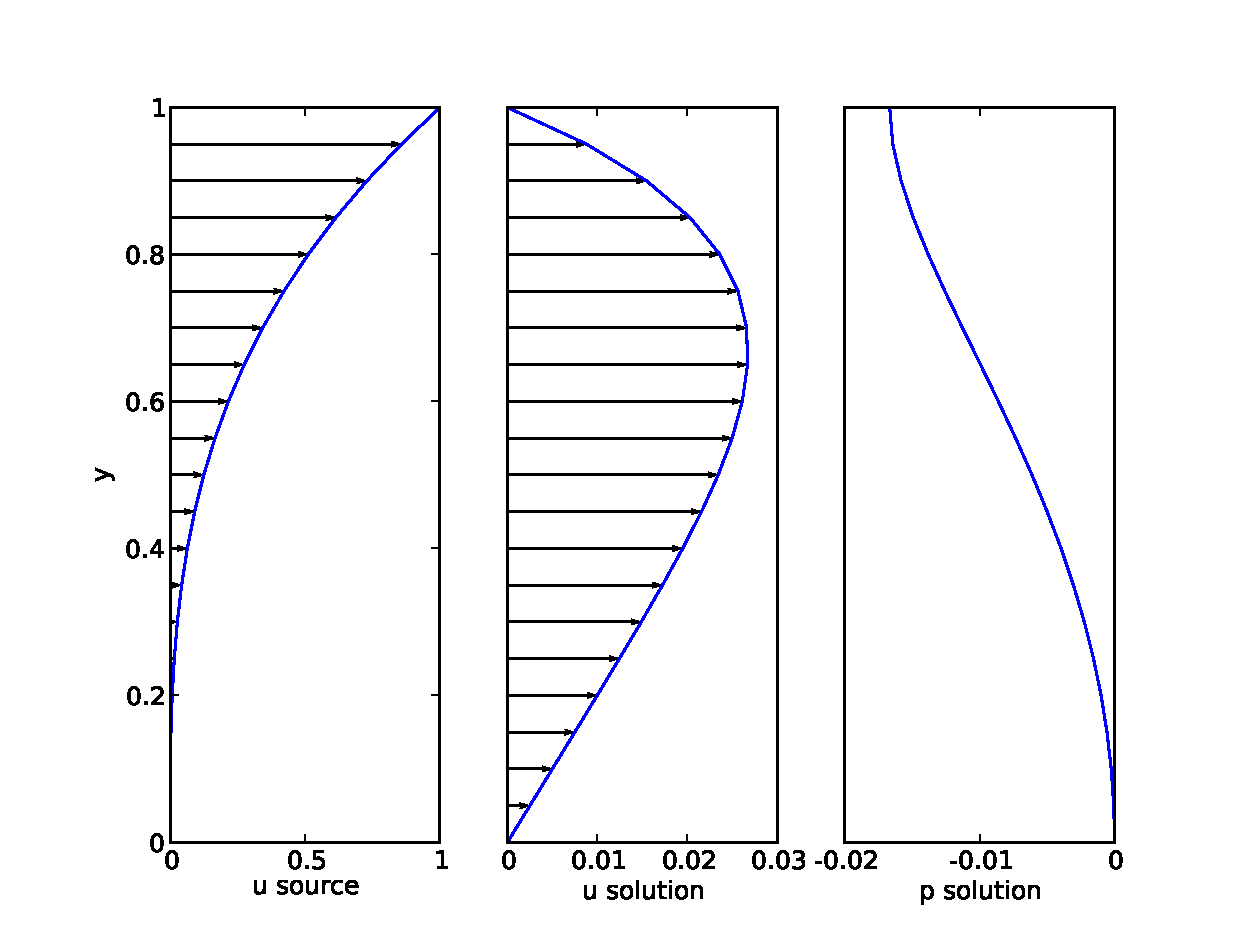
\includegraphics[width=1.1\textwidth]{examples_images/rotating_channel/analytic_solution.eps}
  \onlypdf{\end{pdfdisplay}}
  \caption{Velocity forcing term and analytic solutions for velocity and
    pressure for the rotating periodic channel test case. Note that each of
    these quantities is constant in the $x$ direction.}
  \label{fig:periodic_channel}
\end{figure}

The convergence test is conducted by repeating this simulation on unstructured meshes
with typical resolution $1/4$, $1/8$, $1/16$, $1/32$, $1/64$. The results
are then compared to the analytic solution. In the case of pressure, the
answer is translated to account for the arbitrary constant. Figure
\ref{fig:periodic_channel_error}\ shows the $\textrm{L}^2$ error for
velocity and pressure. It is apparent that both quantities converge at
second order.

\begin{figure}[htbp]
  \centering
  \onlypdf{\begin{pdfdisplay}}
    \psfrag{u error}{$\vec{u}$ error}
    \psfrag{p error}{$p$ error}
    \psfrag{O\(dx^2\)}{$O(\d x^2)$}
    \psfrag{dx}{$\d x$}
    \psfrag{1.0e+00}{\small\hspace{1em}$1$}
    \psfrag{1.0e-01}{\small\hspace{1em}$10^{-1}$}
    \psfrag{1.0e-02}{\small\hspace{1em}$10^{-2}$}
    \psfrag{1.0e-03}{\small\hspace{1em}$10^{-3}$}
    \psfrag{1.0e-04}{\small\hspace{1em}$10^{-4}$}
    \psfrag{1.0e-05}{\small\hspace{1em}$10^{-5}$}
    \psfrag{1.0e-06}{\small\hspace{1em}$10^{-6}$}
    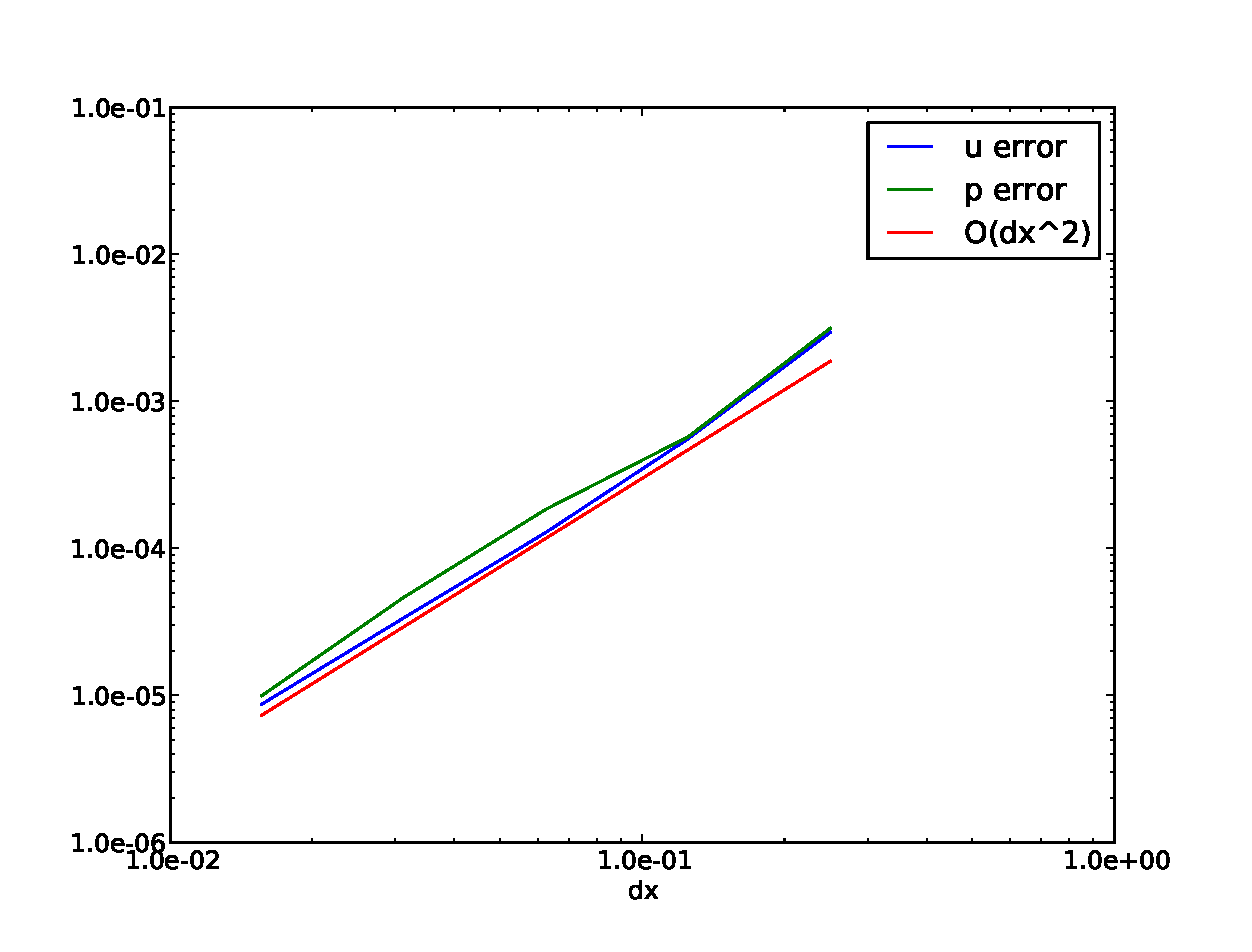
\includegraphics[width=1.1\textwidth]{examples_images/rotating_channel/convergence.eps}
  \onlypdf{\end{pdfdisplay}}  
  \caption{Error in the pressure and velocity solutions for the rotating channel as a function of resolution.}
  \label{fig:periodic_channel_error}
\end{figure}

\subsubsection{Exercises}

This example can be used to understand the use of analytic forcing
functions in \fluidity. Try modifying the function
\lstinline[language=python]{channel_tools.forcing}. The forcing function
and the analytic velocity and pressure results can be visualised by running
the \lstinline[language=python]{plot_theory}\ script. 

Examine the rest of the \lstinline[language=python]{channel_tools}\ Python
module to see how the analytic solution is automatically calculated from the
forcing function. Next, examine the \option{AnalyticUVelocitySolutionError}\
and \option{AnalyticPressureSolutionError} to see how this is used to
calculate the error in the model solution. The documentation of the Python
state interface in appendix \ref{chap:python}\ may be useful.

% %%%%%%%%%%%%%%%%%%%%%%%%%%%%%%%%%%%%%%%%%%%%%%%%%%%%%%%%%%%%%%%%%%%
% %---Open ocean deep convection--------------------%
% %%%%%%%%%%%%%%%%%%%%%%%%%%%%%%%%%%%%%%%%%%%%%%%%%%%%%%%%%%%%%%%%%%%
% 
% \section{Open ocean deep convection}
% \label{sec:OODC}
% \subsection{Overview}
% Open-ocean deep convection (OODC) has been recognised as an
% important mixing process for over 25 years, and
% has been studied in the ocean, simulated in the laboratory, and modelled numerically.
% A much-cited study in the field of numerically simulating
% open-ocean deep convection is that of \cite{jones1993} and this is recreated here.
% In their work, a fixed resolution ($240 \times 240 \times
% 100$m in $X, Y, Z$) model is used to study the physics and
% characteristic scalings of OODC. Their simulations use a disc
% of cooling in a simple box geometry to investigate the effects of rotation.
% 
% Ocean convection is important to the meridional overturning
% circulation. It is a small scale non-hydrostatic process which
% is difficult to capture in general circulation models. Applying
% an unstructured adaptive mesh model to study this process is
% novel, and this approach may produce new insights into the
% simulation and parameterisation of convection in structures and
% unstructured mesh models.
% 
% Although OODC itself is a small-scale process, it interacts with
% processes on the basin-scale, both in the preconditioning stage and
% in the sinking and spreading stages. It is therefore important for us
% to be able to represent a large range of scales. Finite elements and adapting
% unstructured meshes are particularly suited for this application, as the
% resolution used can vary in size smoothly over a wide area.
% 
% \subsection{Configuration}
% 
% \subsubsection{Geometry}
% 
% %\begin{figure}
% %\centering
% %\pdffig[width=8.0cm]{images/oodc-schematic.pdf}
% %\caption{Schematic of the domain for the three-dimensional open ocean deep convection
% %problem.}
% %\label{fig:Schematic}
% %\end{figure}
% 
% 
% A schematic of the domain is shown in figure \ref{fig:Schematic}.
% The domain is 32km square in the horizontal and 2km deep. A cooling disk of radius
% 8km is centred at middle of the upper boundary.
% 
% 
% 
% 
% \subsubsection{Parameters}
% The thermal expansion coefficient is set to
% $\alpha=2 \times 10^{-4} \,\mathrm{K}^{-1}$ and gravity to $g=9.81 \,\mathrm{m}\,\mathrm{s}^{-2}$.
% 
% The eddy viscosity
% and thermal diffusivity were set to the same values as those
% used in \cite{jones1993}: $\kappa_h = 5.0 \mathrm{m}^2\mathrm{s}^{-1}$ and
% $\kappa_v = 0.2 \mathrm{m}^2\mathrm{s}^{-1}$.
% 
% 
% \subsubsection{Initial and boundary conditions}
% The domain is initialised at rest with a weak temperature stratification
% in the vertical, with a top-to-bottom temperature difference of
% $0.05\,$K.
% This therefore corresponds to a buoyancy frequency ($N$) value
% of $2.2 \times 10^{-4} \,\mathrm{s}^{-1}$.
% 
% 
% A heat loss of $-800\,\mathrm{W}\,\mathrm{m}^{-2}$ is
% applied as a flux boundary condition. Assuming density $\rho=1000\,\mathrm{Kg}\,\mathrm{m}^{-3}$,
% specific heat capacity $c_p=4\times 10^3\,\mathrm{J}\,\mathrm{Kg}^{-1}\,\mathrm{K}^{-1}$,
% the flux $q=\bmn\cdot\left ( \kaptens_T  \nabla T\right)$
% takes the value $q = 2\times 10^{-4}\,\mathrm{K}\,\mathrm{m}^{-1}\,\mathrm{s}^{-1}$.
% This value is applied in a disk of radius $7750\,\mathrm{m}$ with a linear ramp to zero flux to a radius
% $8000\,\mathrm{m}$. In addition, this forcing is only applied for the first 48 hours of the simulation and
% then switched off, so that the restratification stage of the problem can be considered.
% 
% 
% 
% No-normal flow, free-stress boundary conditions are applied at the upper and lateral
% (spanwise) boundaries.
% 
% 
% \subsection{Results}
% 
% 
% 

\section{Water column collapse}
\label{sec:water_collapse}

\subsection{Overview}
A commonly used validation experiment for multi-material models is that of a collapsing column of liquid, normally water, within an atmosphere or vacuum \citep{lakehal_interface_2002}, also known as the dam break problem.  In the experimental set-up a reservoir of water is held behind an impermeable barrier separating it from the rest of the tank.  The barrier is then quickly removed, allowing the water column to collapse and flood the remaining sections of the tank.  In the numerical analogue the initial condition is generally taken as the trapped water column, still behind the dam.  At the start of the simulation the barrier is imagined to have been removed instantaneously and switching on gravity, $|g| = 9.81$, causes the column to collapse.   Several experimental set-ups have been published and used as comparison and validation tools for numerical models \citep{martin_part_1952, greaves_simulation_2006}.  Those with water depth gauges distributed throughout the tank are particularly useful, allowing the direct comparison of data.  Furthermore, pressure gauges located on the tank walls or on any obstacles within the tank provide another useful validation tool.

In this example, \fluidity\ is used to simulate a simple dam break experiment \citep{zhou_nonlinear_1999}.  The example demonstrates the following functionality:

\begin{itemize}
\item 2D flow
\item Multi-material flow
\item Incompressible flow
\item Inviscid flow
\item Mesh adaptivity
\item Static detectors
\end{itemize}

The simulation illustrated here took $\sim$2 hours to run in serial on a Intel Xeon X5355 2.66 GHz processor.

\subsection{Problem specification}
The experiment on which this example is based was a simple dam break problem in a $3.22\times2\times1m$ (length $\times$ height $\times$ depth) tank \citep{zhou_nonlinear_1999}.  A reservoir of water $1.2\times0.6\times1m$ (length $\times$ height $\times$ depth) was held behind a barrier at one end of the tank.  Water depth gauges were placed at two points, marked H1 and H2 in Figure \ref{fig:zhouinitial}(a), at $x_1 = 2.725m$ and $2.228m$ respectively.  Additionally, a pressure gauge was located at the point marked P2 in Figure \ref{fig:zhouinitial}(a), at $x_2=0.16m$ on the wall facing the initial water column.

As no variations were introduced in the third dimension, the experiment is reproduced here numerically in two dimensions within the domain $\Omega$: $x_1 \in [0,3.22]$, $x_2 \in [0,2]$ \citep{lee_numerical_2002, colagrossi_numerical_2003, park_volume-of-fluid_2009}.  The two materials (water and air) are distinguished by scalar fields $\alpha_k$ representing their volume fraction, where the volume fraction of air $\alpha_2 = 1-\alpha_1$ and $\alpha_1$ is the volume fraction of water. The initial condition of the water volume fraction is shown in Figure \ref{fig:zhouinitial}(a).  The presence of water is indicated as a blue region and the interface to air is delineated by contours at volume fraction values of $0.025$, $0.5$ and $0.975$.  The densities of the water and air are taken as $ 1,000kg\,m^{-2}$ and $1kg\,m^{-2}$ respectively.  Both fluids are treated inviscidly. As the simulation is inviscid, free slip boundary conditions are imposed on the tank bottom, $x_2=0$, and sides, $x_1=0,\,3.22$.  The top of the tank, $x_2=2$, is left open.

\begin{figure}[tbp]
\hspace{1cm}(a)
\begin{center}
\hspace{0.4cm}\begin{picture}(0,0)%
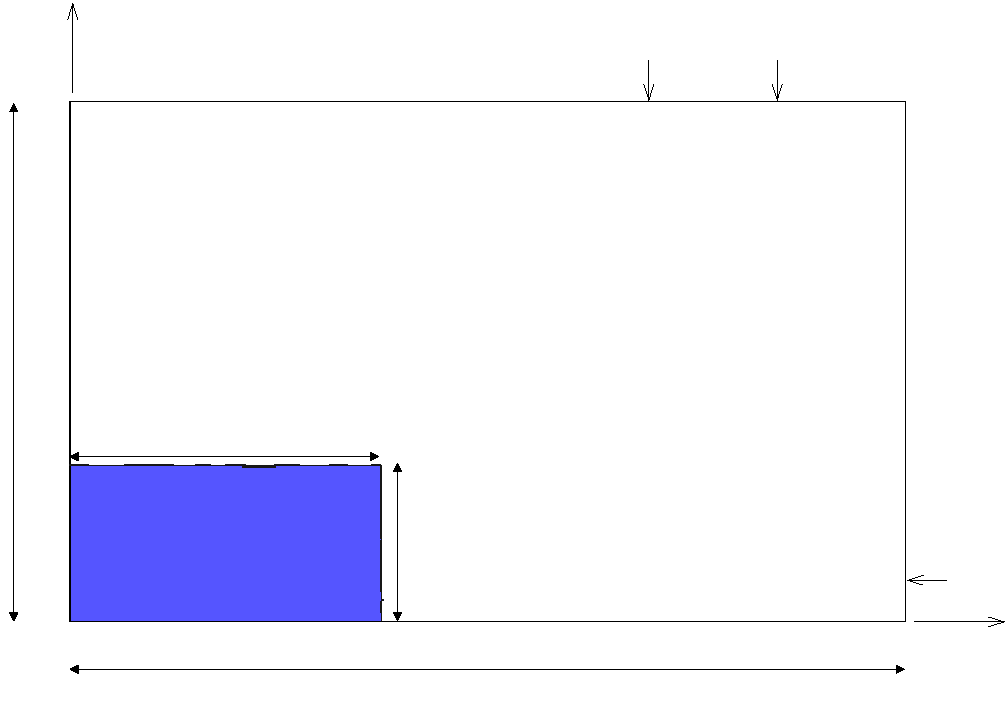
\includegraphics[scale=0.7]{examples_images/water_collapse/initial_setup.pdf}%
\end{picture}%
\setlength{\unitlength}{2900.8sp}%
%
\begingroup\makeatletter\ifx\SetFigFontNFSS\undefined%
\gdef\SetFigFontNFSS#1#2#3#4#5{%
  \reset@font\fontsize{#1}{#2pt}%
  \fontfamily{#3}\fontseries{#4}\fontshape{#5}%
  \selectfont}%
\fi\endgroup%
\begin{picture}(8550,5377)(1531,-9251)
\put(5366,-8836){\makebox(0,0)[lb]{\smash{{\SetFigFontNFSS{10}{12.0}{\familydefault}{\mddefault}{\updefault}{\color[rgb]{0,0,0}$d_in_i = 0$}%
}}}}
\put(2476,-7051){\rotatebox{90.0}{\makebox(0,0)[lb]{\smash{{\SetFigFontNFSS{10}{12.0}{\familydefault}{\mddefault}{\updefault}{\color[rgb]{0,0,0}$d_in_i = 0$}%
}}}}}
\put(5761,-5326){\makebox(0,0)[lb]{\smash{{\SetFigFontNFSS{10}{12.0}{\familydefault}{\mddefault}{\updefault}{\color[rgb]{0,0,0}Air}%
}}}}
\put(2746,-4021){\makebox(0,0)[lb]{\smash{{\SetFigFontNFSS{10}{12.0}{\familydefault}{\mddefault}{\updefault}{\color[rgb]{0,0,0}$x_2$}%
}}}}
\put(5356,-4561){\makebox(0,0)[lb]{\smash{{\SetFigFontNFSS{10}{12.0}{\familydefault}{\mddefault}{\updefault}{\color[rgb]{0,0,0}$p = 0$}%
}}}}
\put(9136,-6191){\rotatebox{270.0}{\makebox(0,0)[lb]{\smash{{\SetFigFontNFSS{10}{12.0}{\familydefault}{\mddefault}{\updefault}{\color[rgb]{0,0,0}$d_in_i = 0$}%
}}}}}
\put(7111,-4246){\makebox(0,0)[b]{\smash{{\SetFigFontNFSS{10}{12.0}{\familydefault}{\mddefault}{\updefault}{\color[rgb]{0,0,0}2.228$m$}%
}}}}
\put(8101,-4246){\makebox(0,0)[b]{\smash{{\SetFigFontNFSS{10}{12.0}{\familydefault}{\mddefault}{\updefault}{\color[rgb]{0,0,0}2.725$m$}%
}}}}
\put(7066,-4021){\makebox(0,0)[b]{\smash{{\SetFigFontNFSS{10}{12.0}{\familydefault}{\mddefault}{\updefault}{\color[rgb]{0,0,0}H2}%
}}}}
\put(8056,-4021){\makebox(0,0)[b]{\smash{{\SetFigFontNFSS{10}{12.0}{\familydefault}{\mddefault}{\updefault}{\color[rgb]{0,0,0}H1}%
}}}}
\put(9586,-8881){\makebox(0,0)[lb]{\smash{{\SetFigFontNFSS{10}{12.0}{\familydefault}{\mddefault}{\updefault}{\color[rgb]{0,0,0}$x_1$}%
}}}}
\put(9676,-8341){\makebox(0,0)[b]{\smash{{\SetFigFontNFSS{10}{12.0}{\familydefault}{\mddefault}{\updefault}{\color[rgb]{0,0,0}0.16$m$}%
}}}}
\put(9676,-8116){\makebox(0,0)[b]{\smash{{\SetFigFontNFSS{10}{12.0}{\familydefault}{\mddefault}{\updefault}{\color[rgb]{0,0,0}P2}%
}}}}
\put(5761,-9196){\makebox(0,0)[b]{\smash{{\SetFigFontNFSS{10}{12.0}{\familydefault}{\mddefault}{\updefault}{\color[rgb]{0,0,0}3.22$m$}%
}}}}
\put(2116,-6631){\makebox(0,0)[rb]{\smash{{\SetFigFontNFSS{10}{12.0}{\familydefault}{\mddefault}{\updefault}{\color[rgb]{0,0,0}2.0$m$}%
}}}}
\put(4051,-7261){\makebox(0,0)[rb]{\smash{{\SetFigFontNFSS{10}{12.0}{\familydefault}{\mddefault}{\updefault}{\color[rgb]{0,0,0}1.2$m$}%
}}}}
\put(5446,-8071){\makebox(0,0)[b]{\smash{{\SetFigFontNFSS{10}{12.0}{\familydefault}{\mddefault}{\updefault}{\color[rgb]{0,0,0}0.6$m$}%
}}}}
\put(3601,-7036){\makebox(0,0)[lb]{\smash{{\SetFigFontNFSS{10}{12.0}{\familydefault}{\mddefault}{\updefault}{\color[rgb]{0,0,0}Water}%
}}}}
\end{picture}%

\end{center}
\hspace{1cm}(b)
\begin{center}
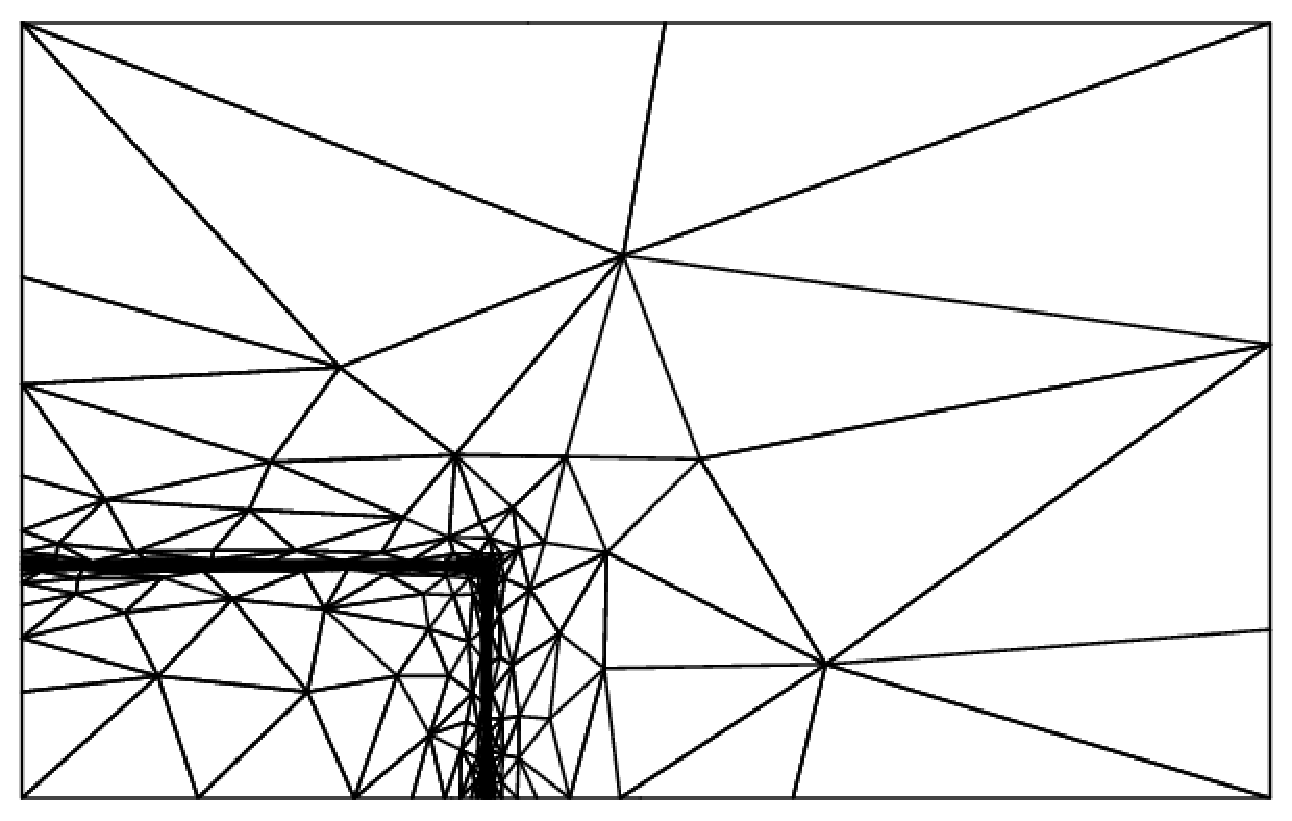
\includegraphics[width=10.4cm, clip=true]{examples_images/water_collapse/water_collapse_0_mesh.pdf}
\end{center}
\caption{(a) Initial set-up of the water volume fraction, $\alpha_1$, and the velocity and pressure boundary conditions for the two-dimensional water column collapse validation problem \citep{zhou_nonlinear_1999}. The presence of water is indicated as a blue region and the interface to air is delineated by contours of the volume fraction at $0.025$, $0.5$ and $0.975$.  The locations of the pressure (P2) and water depth gauges (H1, H2) are also indicated. (b) The adapted mesh used to represent the initial conditions.}
\label{fig:zhouinitial}
\end{figure}

The water volume fraction, $\alpha_1$, is solved for using an advection equation (section~\ref{sec:MP-AdvdifEqn}).  It is advected
using HyperC on a control volume mesh (section~\ref{sec:hyperc}), while the velocity and pressure are discretised using the
$\PzoCV$ element pair (section~\ref{sec:velocity_pressure_element_pairs}) with $\theta=1/2$ and $\theta_i=1/2$ (section~\ref{sec:ND_time_theta_scheme}).  

This example employs an adaptive mesh (chapter~\ref{chap:Adaptivity}). The minimum edge length in the mesh is constrained to $3.33mm$. The upper bound on the edge lengths was specified as half the domain length and height in each dimension.  The water volume fraction was directly adapted to using an interpolation error bound, $\hat{\epsilon}$, of $0.075$. Given the range of this field seen in the fixed mesh runs this corresponds to a desired error of less than 5\%. The volume fraction is transferred between successive meshes using a minimally diffusive bounded projection algorithm.  The velocity is transferred using a straightforward projection while the pressure is consistently interpolated using the linear basis functions from its parent mesh. For details of the remaining adaptivity settings we refer to the documented flml file.  The initial mesh using these settings is shown in Figure \ref{fig:zhouinitial}(b). 

The timestep is selected to achieve a Courant number of $2.5$ while the advection equation uses approximately $10$ subcycles
(section~\ref{sec:cvtemp}) so the volume fraction is advected at a Courant number of $0.25$.  

\subsection{Results}
Several timesteps of the example simulation can be seen in Figure \ref{fig:zhouwholea} where the interface is represented by
contours of the water volume fraction, $\alpha_1$, at $0.025$, $0.5$ and $0.975$.  Similar images can be generated by visualising
the vtu files using Paraview or Mayavi2, see the \href{http://amcg-www.ese.ic.ac.uk/}{AMCG website}\ for more information.

\begin{figure}[tbp]
\begin{center}
% \newcolumntype{V}{>{\centering\arraybackslash} m{7cm} }
\begin{tabular}{ll}
(a) $t = 0.5$ & (b) $t = 1.0$   \\
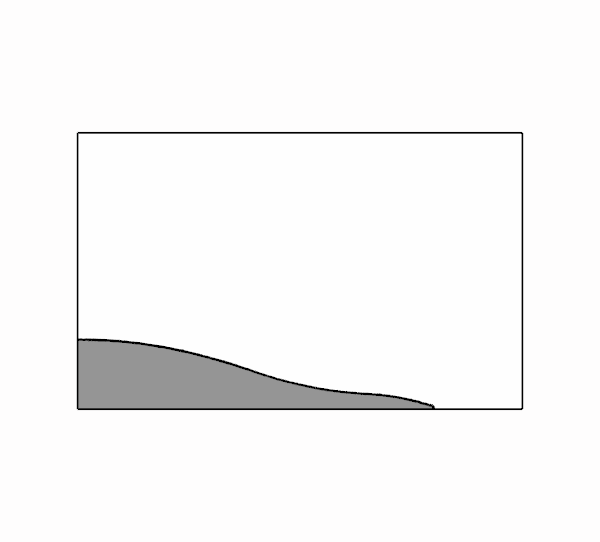
\includegraphics[width=7cm, trim=8.0cm 6.5cm 8.0cm 6.5cm, clip=true]{examples_images/water_collapse/water_collapse_100.png} & 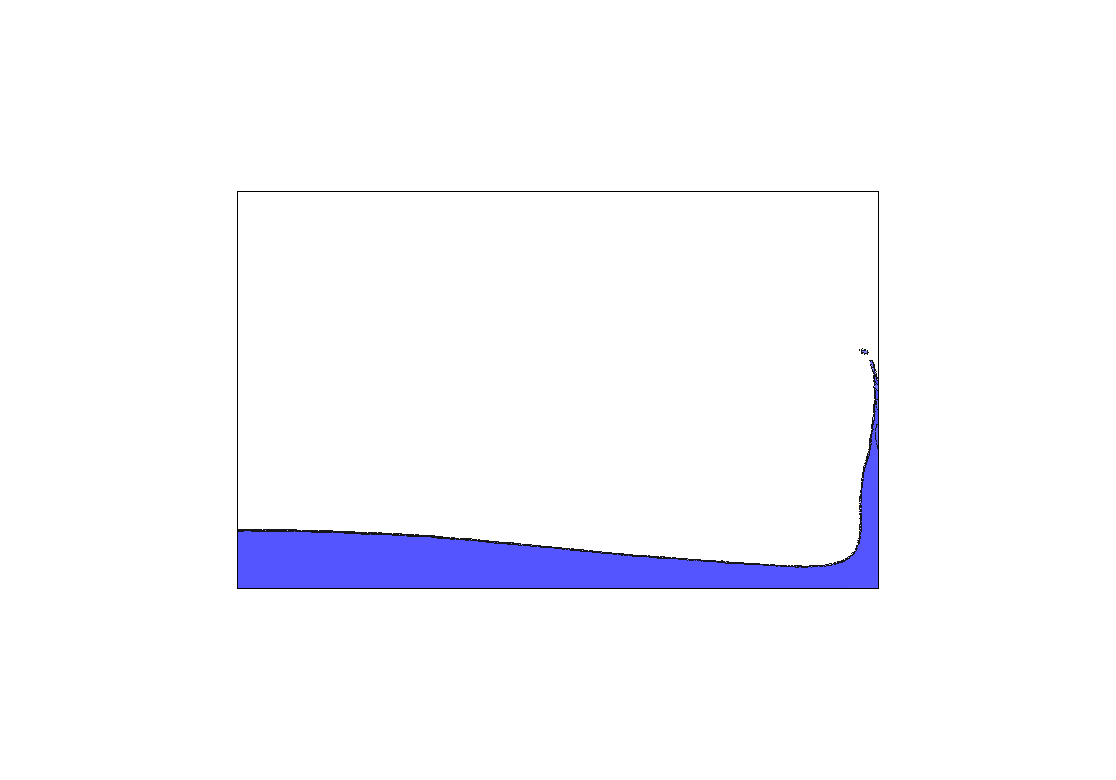
\includegraphics[width=7cm, trim=8.0cm 6.5cm 8.0cm 6.5cm, clip=true]{examples_images/water_collapse/water_collapse_200.png} \\
(c) $t = 1.25$ & (d) $t = 1.5$ \\
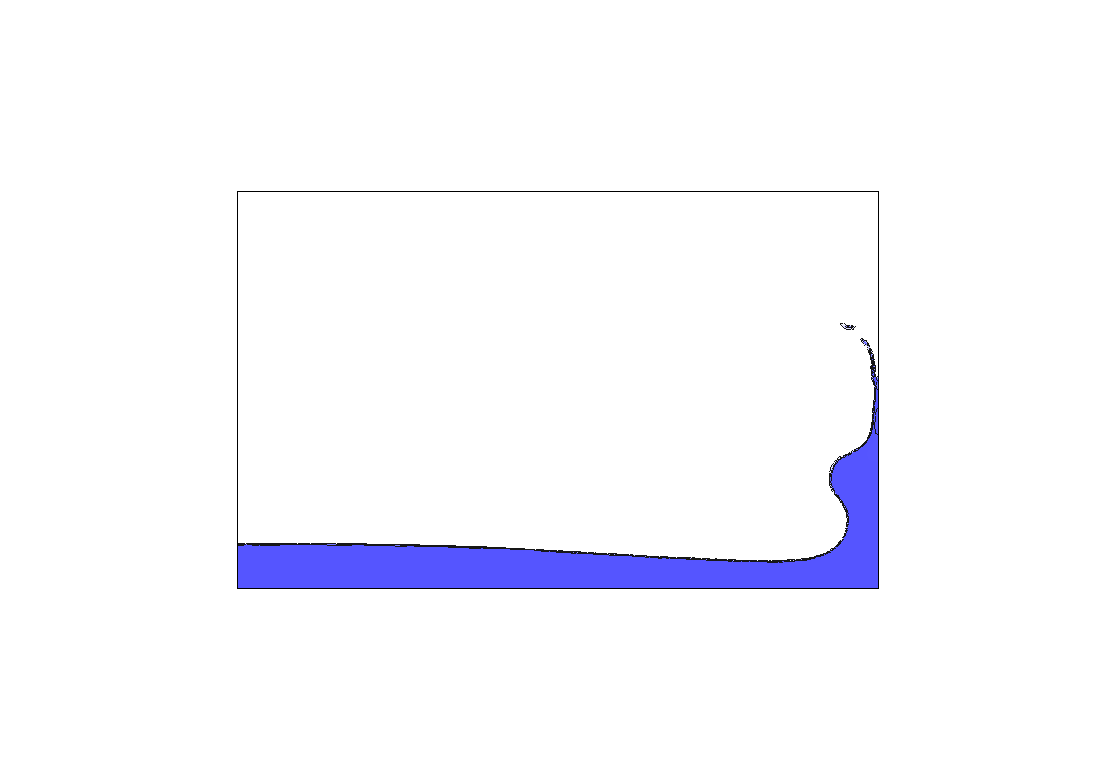
\includegraphics[width=7cm, trim=8.0cm 6.5cm 8.0cm 6.5cm, clip=true]{examples_images/water_collapse/water_collapse_250.png} & 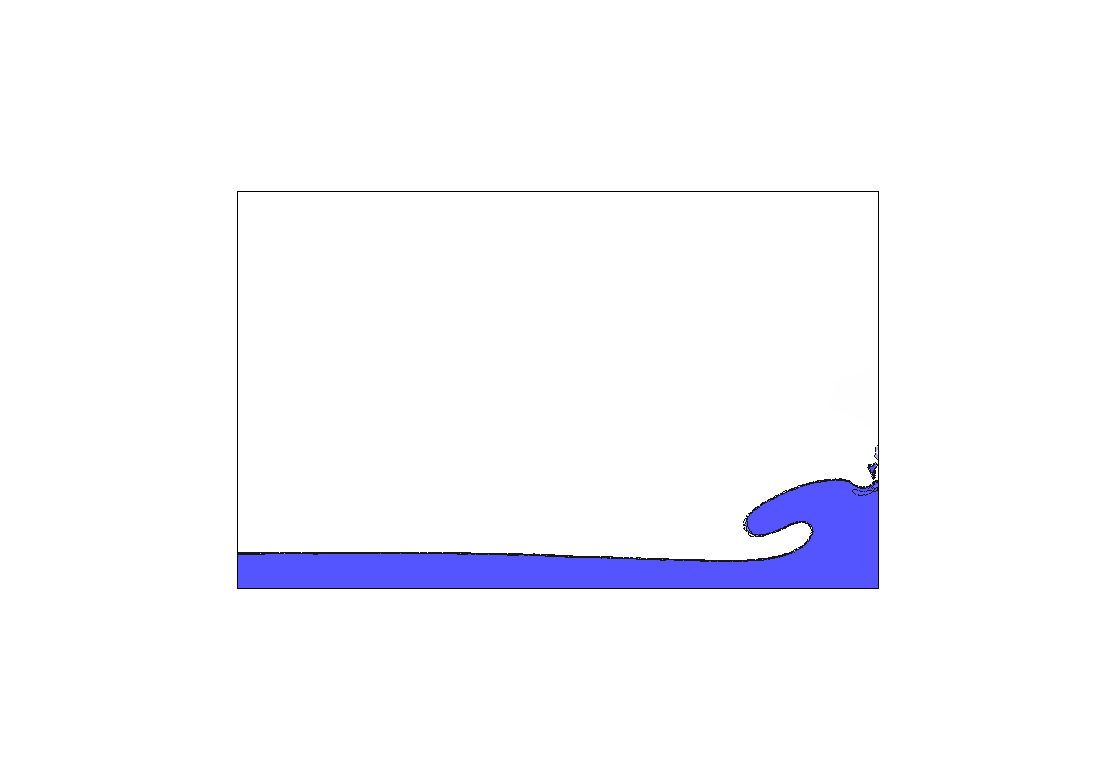
\includegraphics[width=7cm, trim=8.0cm 6.5cm 8.0cm 6.5cm, clip=true]{examples_images/water_collapse/water_collapse_300.png} \\
(e) $t = 1.75$ & (f) $t = 2.0$ \\
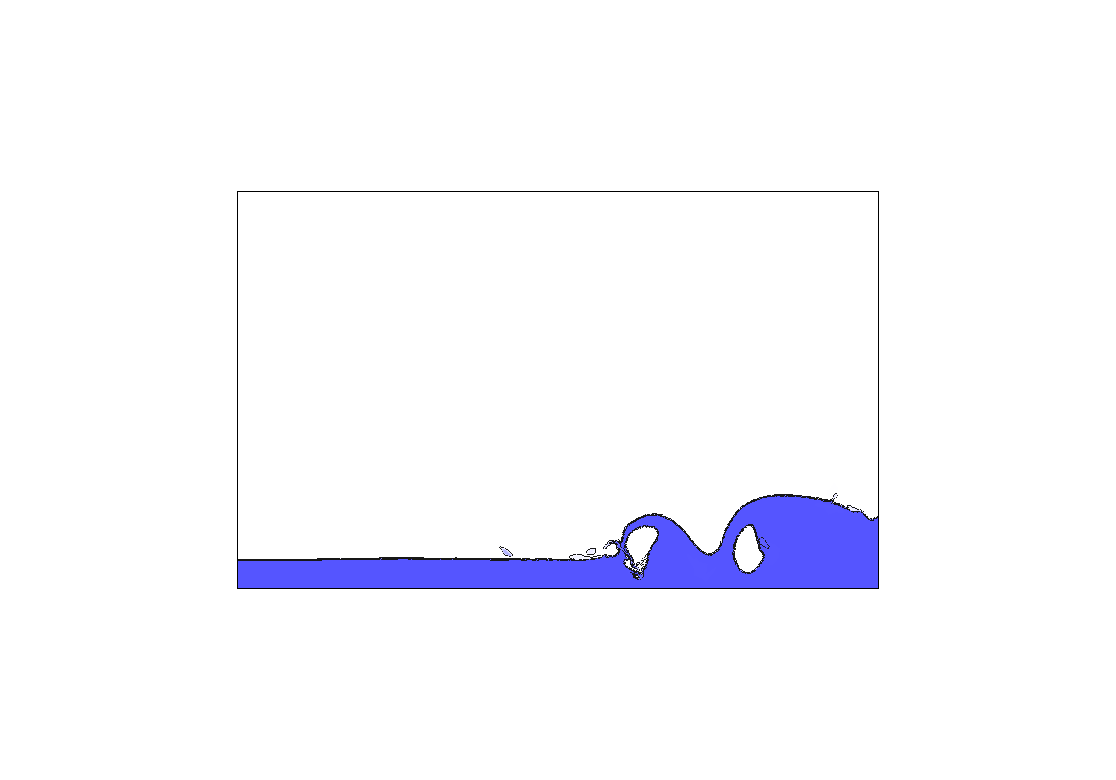
\includegraphics[width=7cm, trim=8.0cm 6.5cm 8.0cm 6.5cm, clip=true]{examples_images/water_collapse/water_collapse_350.png} & 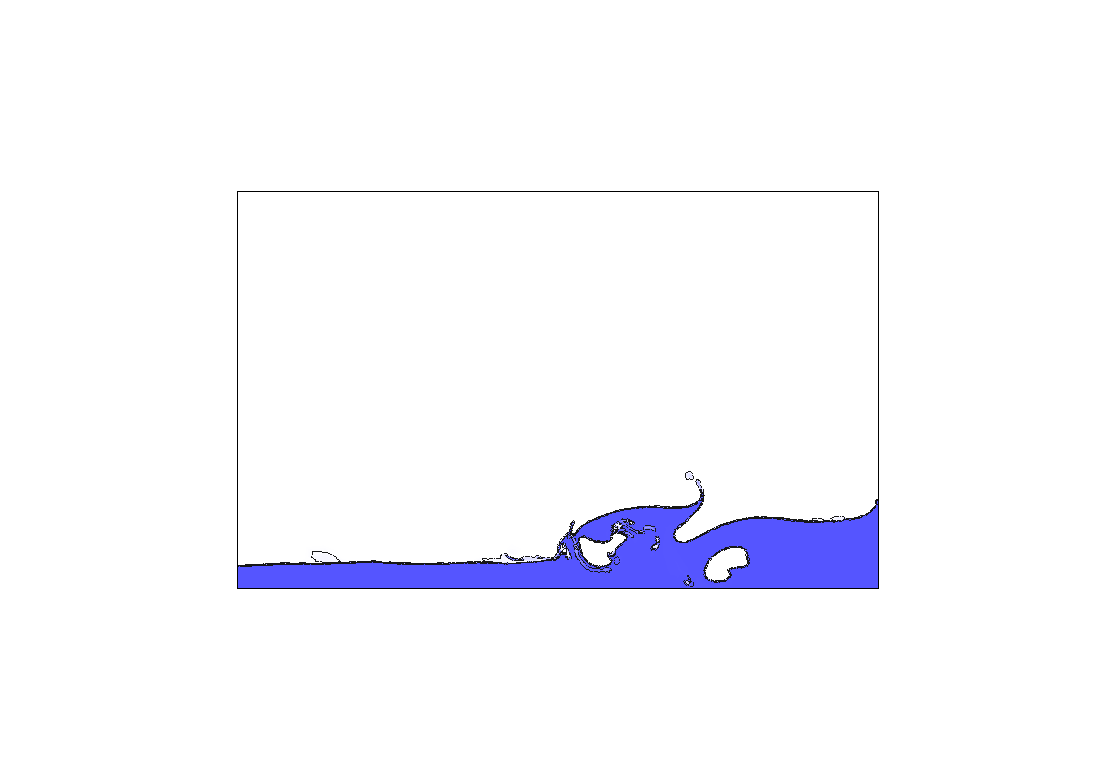
\includegraphics[width=7cm, trim=8.0cm 6.5cm 8.0cm 6.5cm, clip=true]{examples_images/water_collapse/water_collapse_400.png} \\
(g) $t = 2.25$ & (h) $t = 2.5$ \\
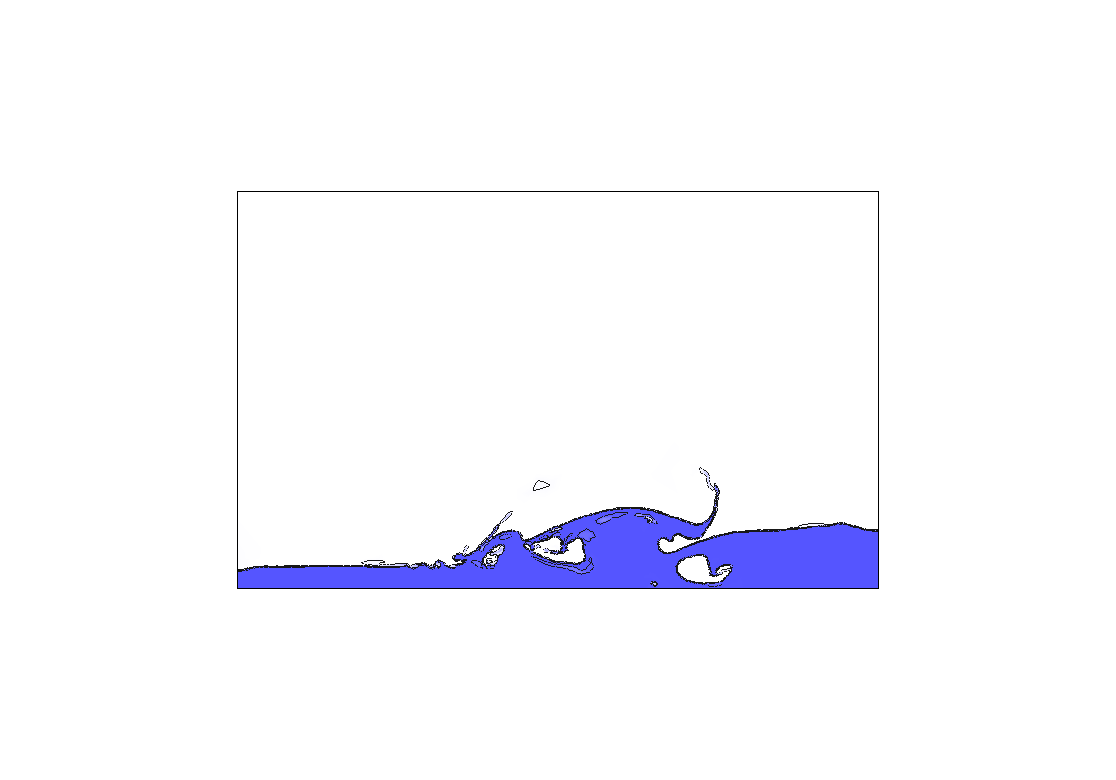
\includegraphics[width=7cm, trim=8.0cm 6.5cm 8.0cm 6.5cm, clip=true]{examples_images/water_collapse/water_collapse_450.png} & 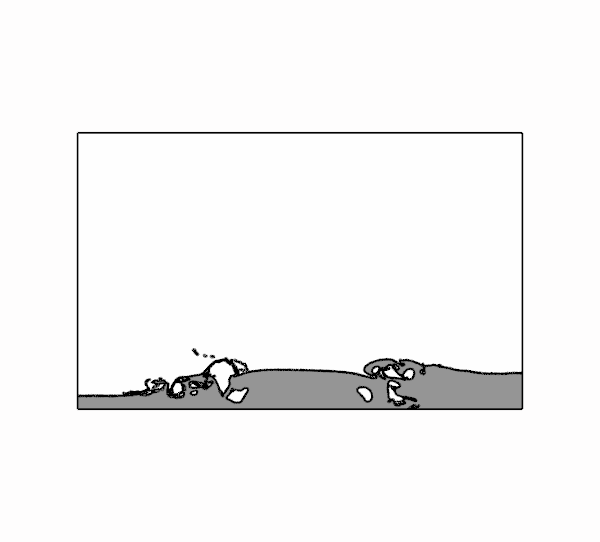
\includegraphics[width=7cm, trim=8.0cm 6.5cm 8.0cm 6.5cm, clip=true]{examples_images/water_collapse/water_collapse_500.png} \\
\end{tabular}
\caption{The evolution of the water volume fraction, $\alpha_1$, over several timesteps.  The presence of water, $\alpha_1=1$, is indicated as a blue region and the interface to air, $\alpha_1=0$, is delineated by contours at $\alpha_1 = 0.025$, $0.5$ and $0.975$.}
\label{fig:zhouwholea}
\end{center}
\end{figure}

\begin{figure}[tbp]
\begin{center}
% \newcolumntype{V}{>{\centering\arraybackslash} m{7cm} }
\begin{tabular}{ll}
(a) $t = 0.5$ & (b) $t = 1.0$\\
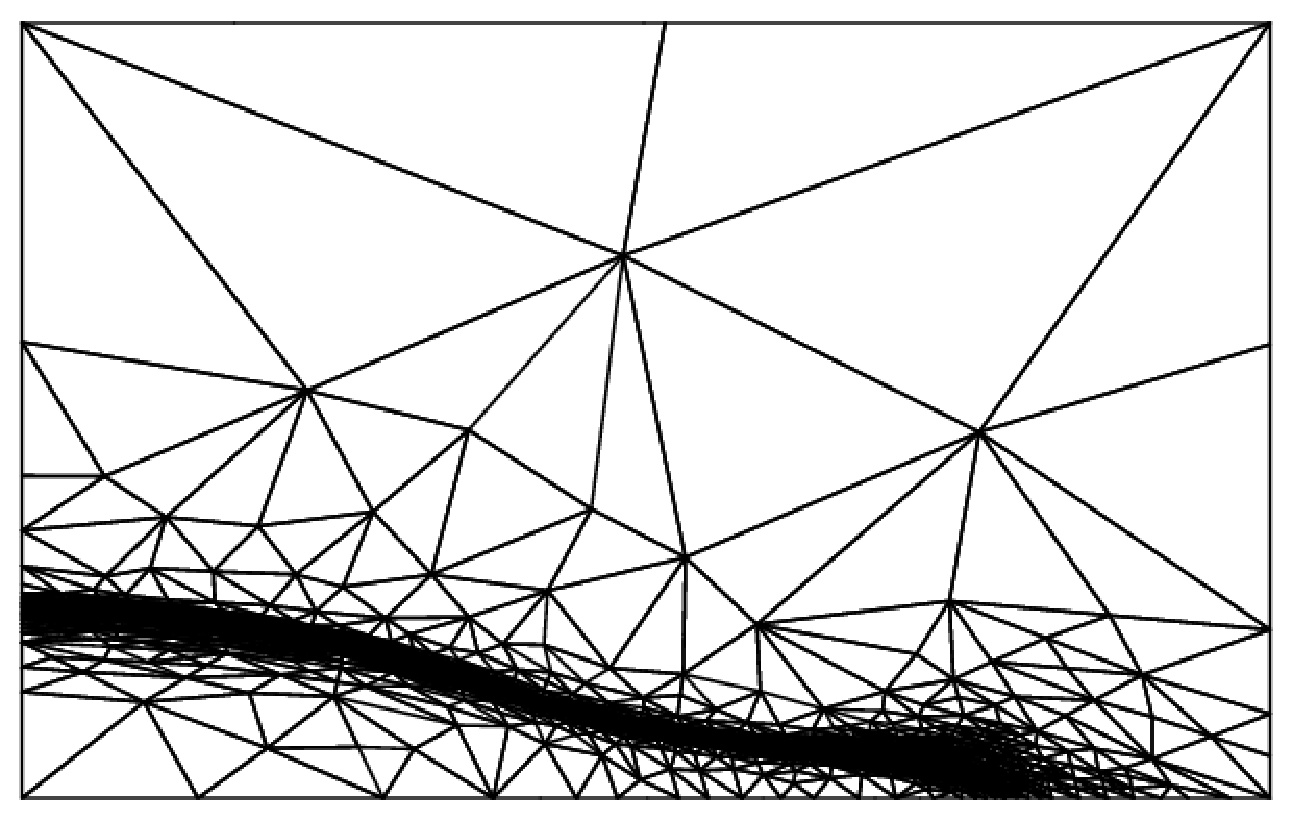
\includegraphics[width=7cm, clip=true]{examples_images/water_collapse/water_collapse_100_mesh.pdf} & 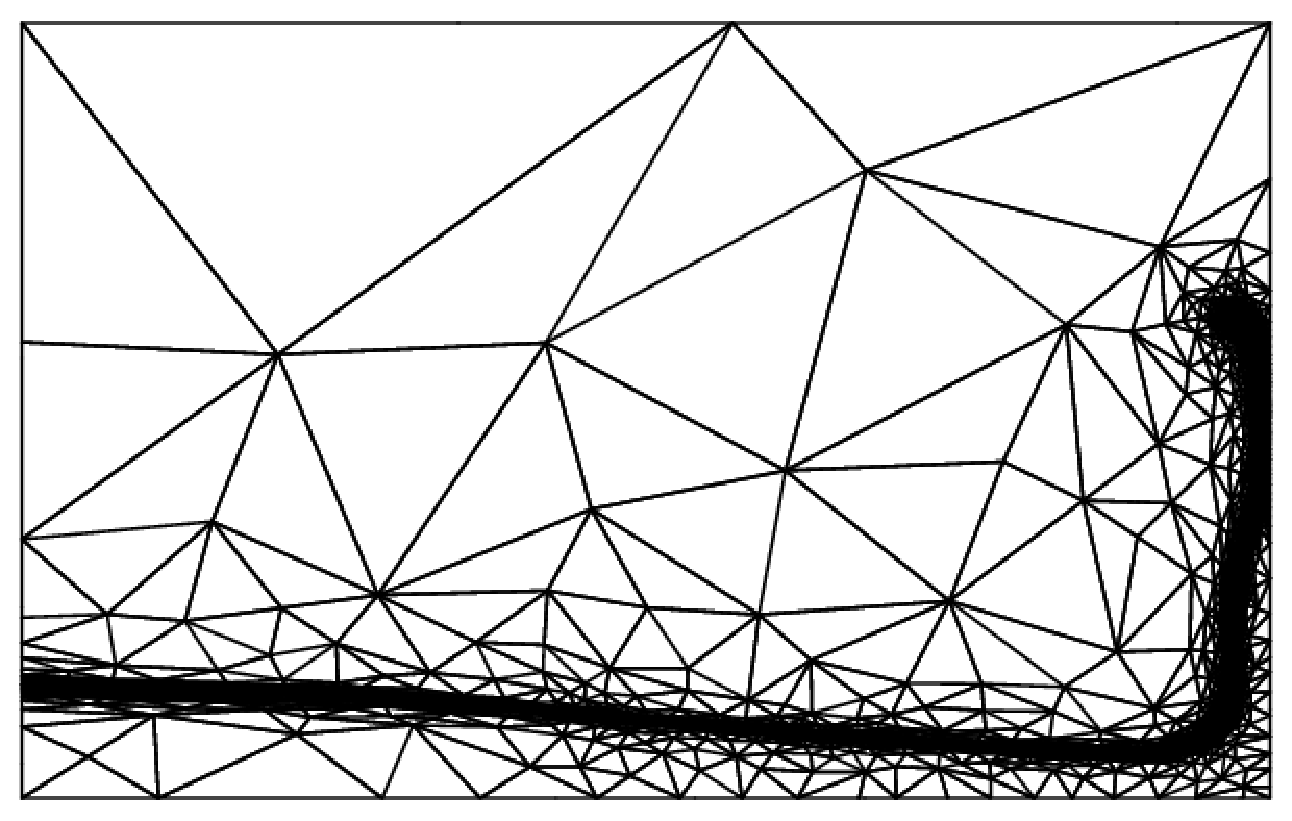
\includegraphics[width=7cm, clip=true]{examples_images/water_collapse/water_collapse_200_mesh.pdf} \\
(c) $t = 1.25$ & (d) $t = 1.5$ \\
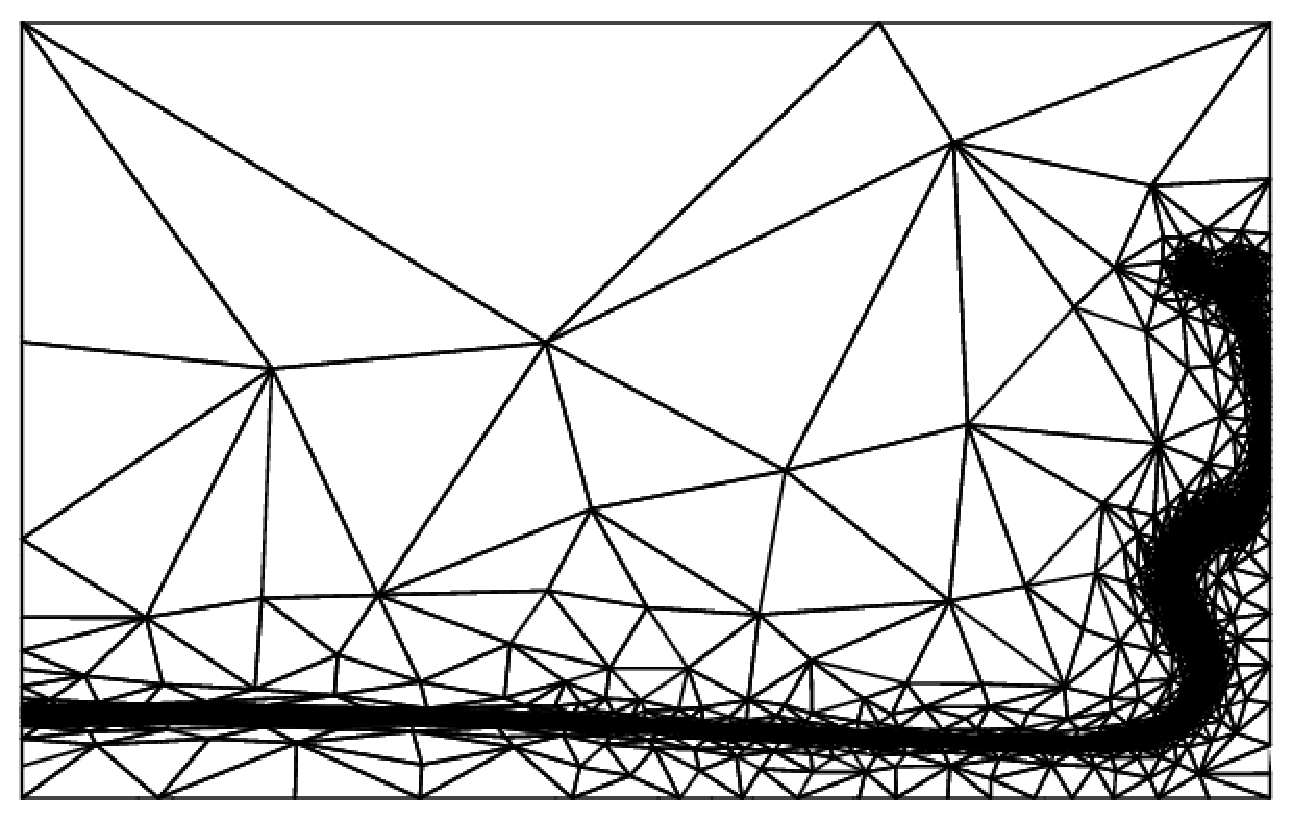
\includegraphics[width=7cm, clip=true]{examples_images/water_collapse/water_collapse_250_mesh.pdf} & 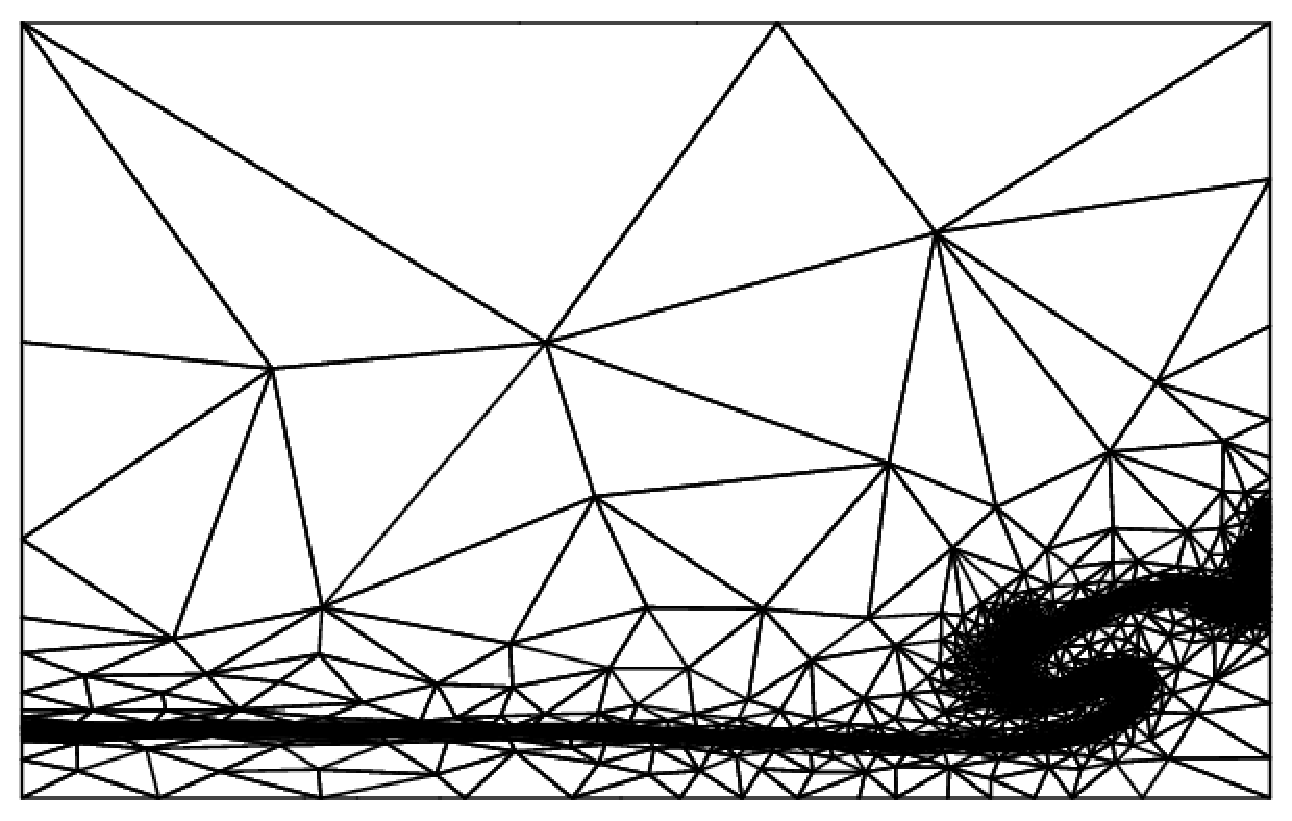
\includegraphics[width=7cm, clip=true]{examples_images/water_collapse/water_collapse_300_mesh.pdf} \\
(e) $t = 1.75$ & (f) $t = 2.0$ \\
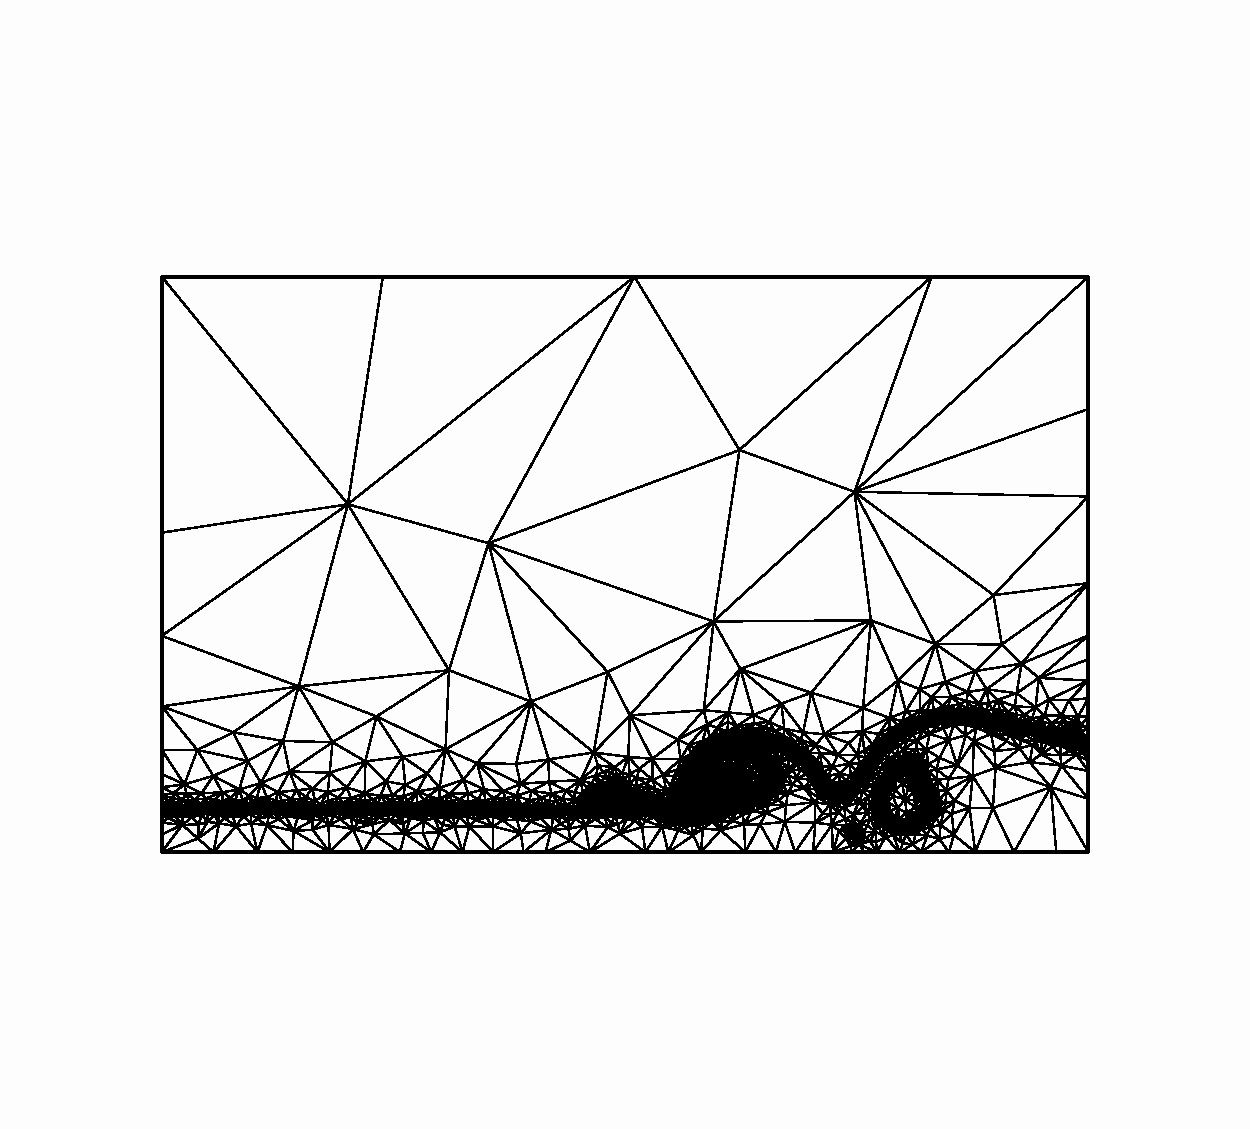
\includegraphics[width=7cm, clip=true]{examples_images/water_collapse/water_collapse_350_mesh.pdf} & 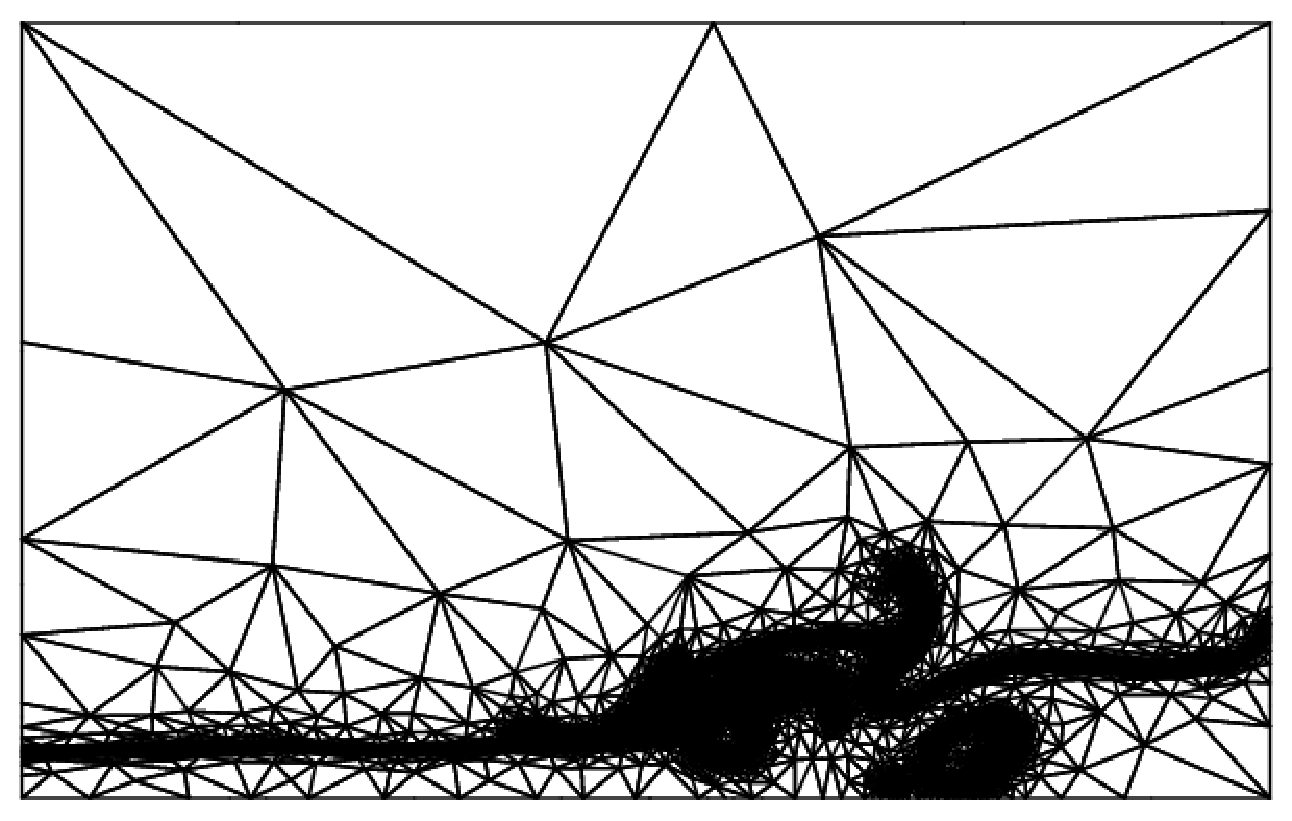
\includegraphics[width=7cm, clip=true]{examples_images/water_collapse/water_collapse_400_mesh.pdf} \\
(g) $t = 2.25$ & (h) $t = 2.5$ \\
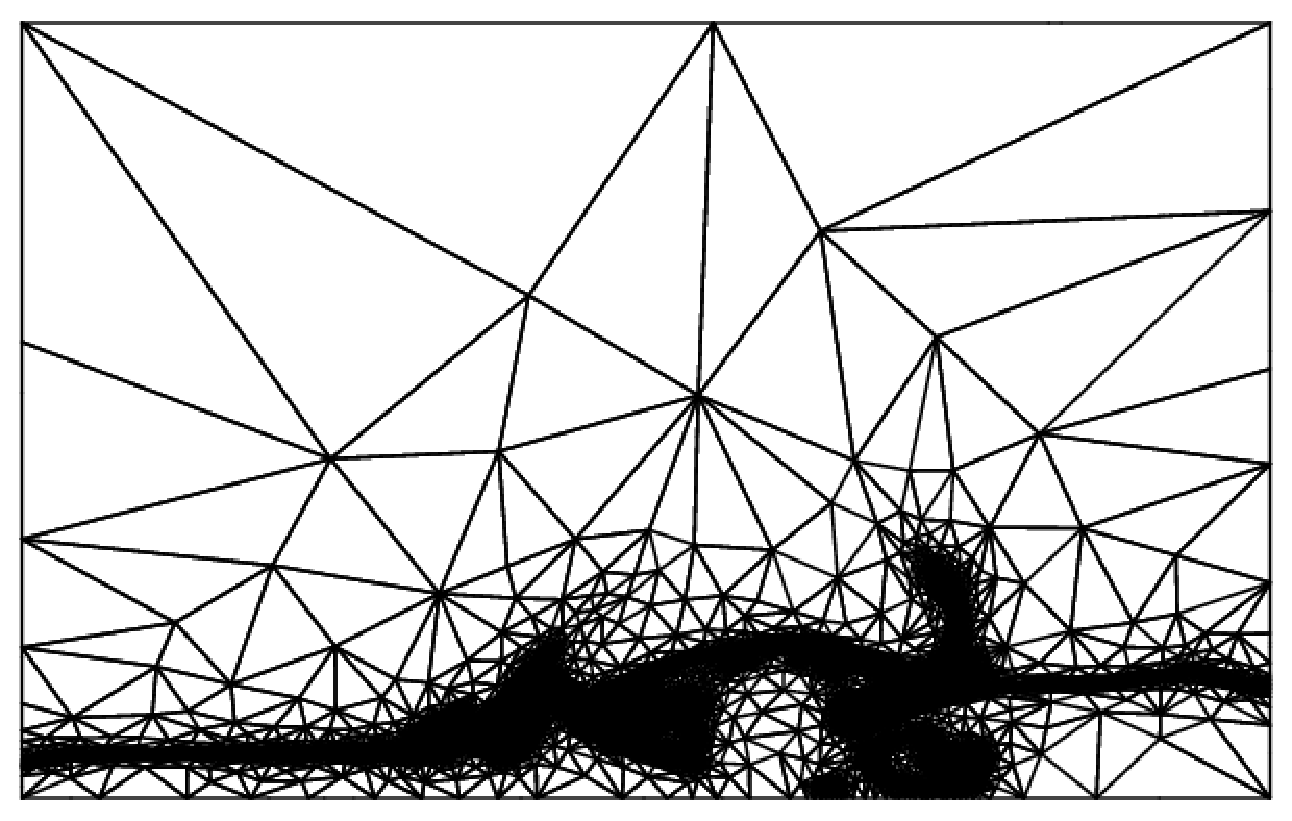
\includegraphics[width=7cm, clip=true]{examples_images/water_collapse/water_collapse_450_mesh.pdf} & 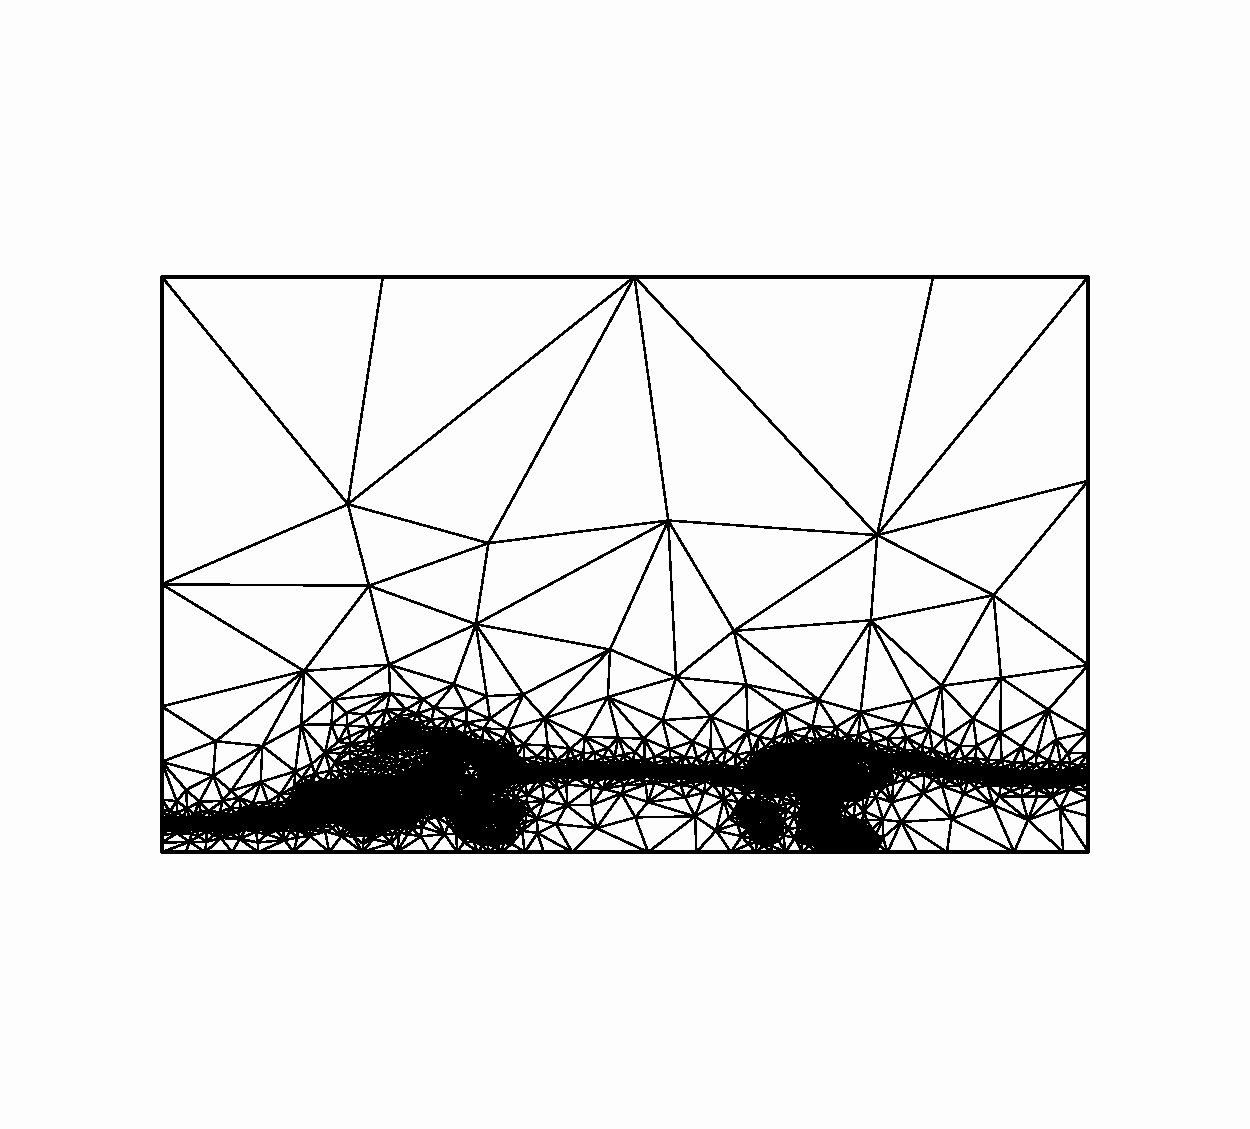
\includegraphics[width=7cm, clip=true]{examples_images/water_collapse/water_collapse_500_mesh.pdf} \\
\end{tabular}
\caption{The evolution of the adaptive mesh over the same timesteps displayed in Figure \ref{fig:zhouwholea}.  The mesh can be seen to closely follow the interface between the water and air.}
\label{fig:zhouwholemesh}
\end{center}
\end{figure}

The images show the column collapse (Figure \ref{fig:zhouwholea}(a)), run-up against the opposing wall (Figure \ref{fig:zhouwholea}(b, c)) and the subsequent overturning wave (Figure \ref{fig:zhouwholea}(d)) and entrainment of air bubbles (Figure \ref{fig:zhouwholea}(e--h)). The evolution of the adaptive mesh over the same timesteps is shown in Figure \ref{fig:zhouwholemesh}. 

\begin{figure}[tbp]
\begin{center}
%\newcolumntype{V}{ m{7cm} }
\begin{tabular}{cc}
\hspace{1cm}(i) H1 & (ii) H2  \\
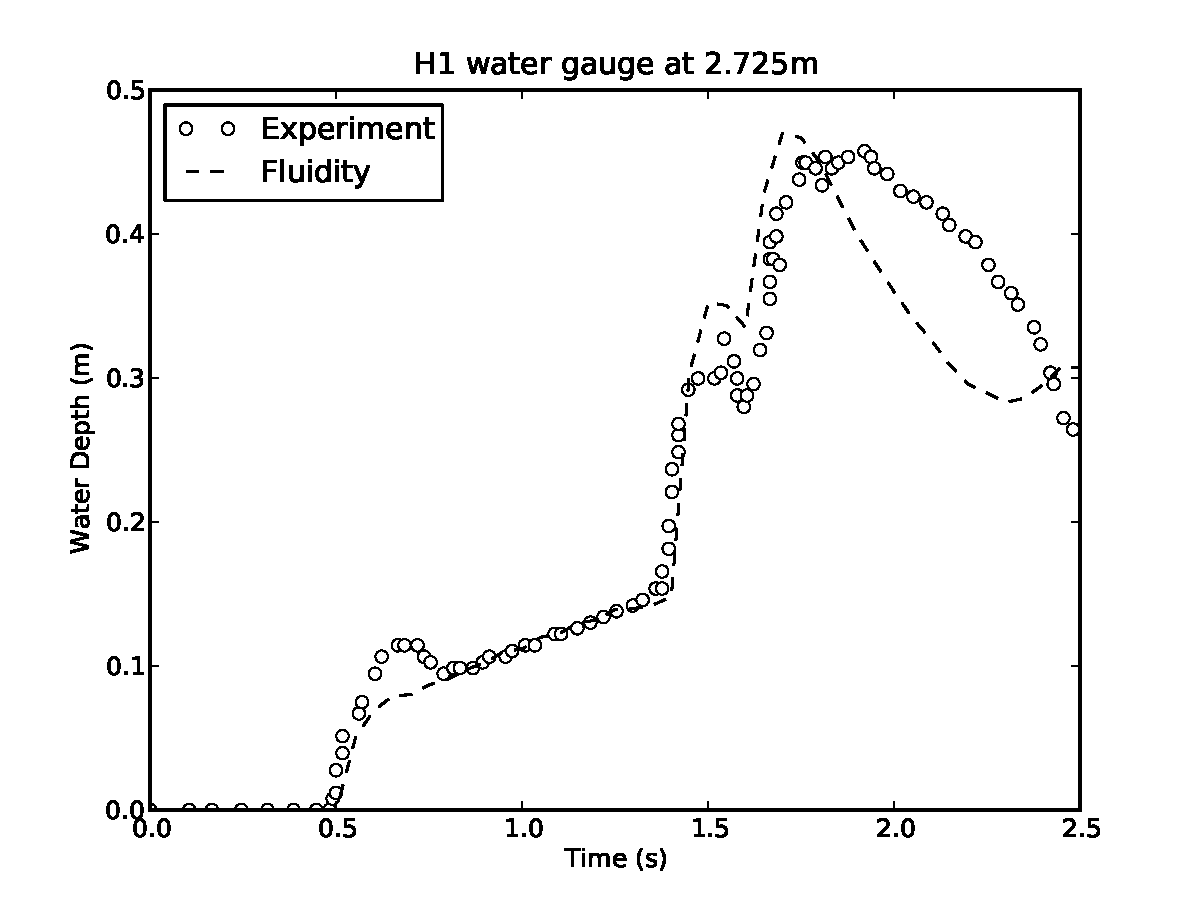
\includegraphics[width=7cm]{examples_images/water_collapse/water_gauge_H1.pdf} & 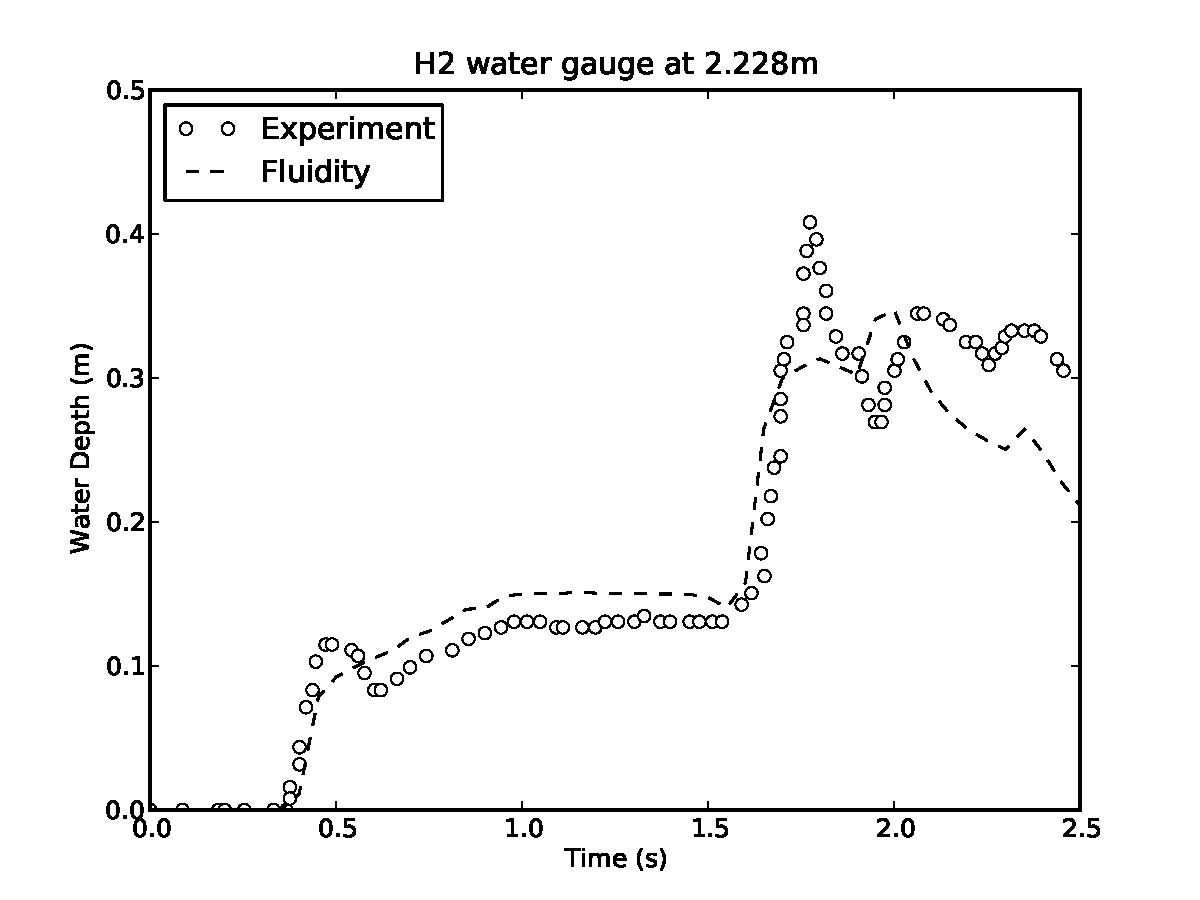
\includegraphics[width=7cm]{examples_images/water_collapse/water_gauge_H2.pdf}\\
\end{tabular}
\caption{Comparison between the experimental (circles) and numerical water gauge data at H1 (i) and H2 (ii), $x_1 = 2.725m$ and $2.228m$ respectively. Experimental data taken from \citet{zhou_nonlinear_1999} through \citet{park_volume-of-fluid_2009}.}
\label{fig:zhoudepth}
\end{center}
\end{figure}

For validation purposes, the post-processing script provided for this example extracts information from the detector file (pressure) and from the water volume fraction field stored in the vtu files (water depth) and plots these data in comparison with the experimental results. The water depth gauge data is displayed in Figure \ref{fig:zhoudepth} alongside the experimental data.  The numerical results show the total thickness of water at the points H1 and H2, discounting any air bubbles that cross the gauges.  The simulation results show a close similarity to the experimental results with the exception of a small lip of water when the initial water head passes the gauge.  It is unclear what causes this structure, though it may be related to the initial withdrawal of the barrier in the experiment or drag effects from the bottom of the tank.  All previous published attempts to model the experiment also fail to reproduce this initial lip \citep{zhou_nonlinear_1999, lee_numerical_2002, colagrossi_numerical_2003, park_volume-of-fluid_2009}.

After $t=1.5s$ the overturning wave starts to pass the water gauges and the match between the experimental results and the numerical simulation deteriorates. As would be expected from such complex behaviour, all previous published attempts have also failed to reproduce the experimental depth gauge data after this point.  However, the broad pattern and average depth observed in the simulation after $t=1.5s$ can be seen in Figure \ref{fig:zhoudepth} to match the experiment reasonably well.

\begin{figure}[tb]
\begin{center}
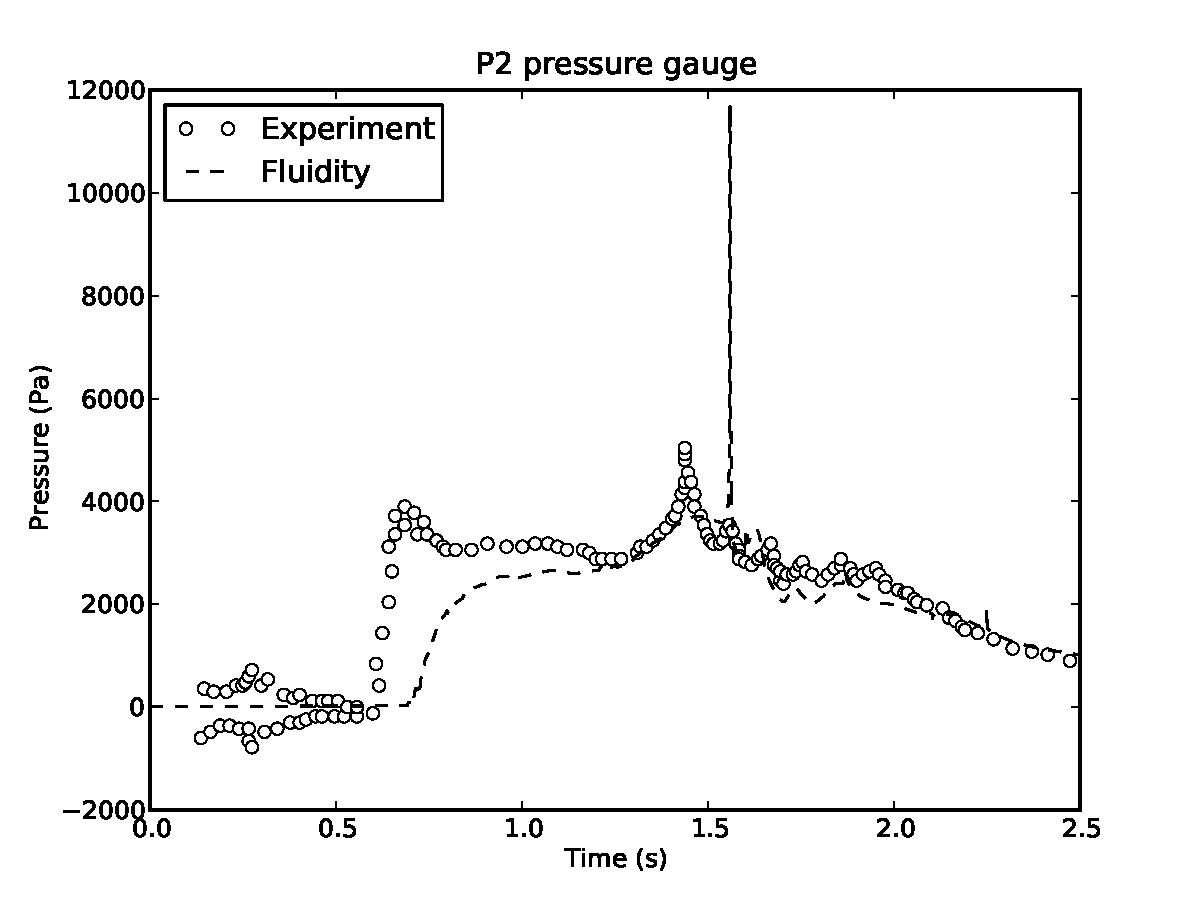
\includegraphics[width=10cm]{examples_images/water_collapse/pressure_gauge_P2.pdf}
\caption{Comparison between the experimental (circles) and numerical pressure gauge data at P2, $x_1 = 3.22m$, $x_2 = 0.16m$. Experimental data taken from \citet{zhou_nonlinear_1999} through \citet{park_volume-of-fluid_2009}.}
\label{fig:zhoupressure}
\end{center}
\end{figure}

Experimental pressure gauge data are also available at the point P2, $(3.22,0.16)m$, on the right wall of the tank.  This is compared to the numerical pressure results in Figure \ref{fig:zhoupressure}.  After the initial noise in the experimental data, a sudden step in pressure is seen as the water run-up reaches the pressure gauge at about $t=0.6s$.  This is also seen in the numerical simulations however it is slightly delayed, occurring at $t=0.7s$.  As upwinding is being used in the discretisation of the velocity field, the delay may be due to numerical viscosity slowing the advancing water front.  However, as the delay was not as extreme at the depth gauges H1 and H2 other factors may also play a role.  For instance, if the lip seen in the experimental water gauge data is a head on the water front, that has not been reproduced numerically, it may reach the height of the pressure gauge faster than a front with no head.

Once the pressure jump occurs the experimental and numerical data are in broad agreement until the overturning wave impacts with the water layer at approximately $t=1.5s$ (Figure \ref{fig:zhouwholea}(d)).  At the point of contact a pressure pulse is transmitted to the pressure gauge resulting in a modest pressure spike in the experimental data.  This is matched by slightly delayed pressure pulses in all the numerical simulation.  However, the pulses seen in the numerical data are of a much larger magnitude than the experimental data. This discrepancy may be due to the fact that in the experiment the pressure gauge measures the pressure over a broader area than in the simulation. 

\subsection{Exercises}
To explore the functionality of \fluidity, the following variations on this example would be constructive learning exercises:

\begin{itemize}
\item Disable the adaptivity option to run on a fixed mesh
\item Alter the water/air viscosity/density
\item Modify the tank geometry
\end{itemize}


%%%%%%%%%%%%%%%%%%%%%%%%%%%%%%%%%%%%%%%%%%%%%%%%%%%%%%%%%%%%%%%%%%%%%%%%%
%%%%%%%%%%%%%%%%%%%%% Restratification after oodc %%%%%%%%%%%%%%%%%%%%%%%
%%%%%%%%%%%%%%%%%%%%%%%%%%%%%%%%%%%%%%%%%%%%%%%%%%%%%%%%%%%%%%%%%%%%%%%%%



\section{The restratification following open ocean deep convection}
\label{sec:restratification_after_oodc}

\subsection{Overview}

During Open Ocean Deep Convection (OODC), cold water is mixed up to the surface via vigorous convection, forming a column of dense water tens of kilometres across known as a convection chimney. This happens in particular sites of the ocean, including the Labrador Sea, the Mediterranean Sea and the Weddell Sea.  In the North Atlantic, the convection typically happens in winter and is triggered by intense cooling at the surface. The convection is important to the formation of North Atlantic Deep Water, which joins the southward part of the Atlantic Meridional Overturning Circulation (AMOC).

It is thought that OODC could be affected by future climate change. If ice caps melt or the hydrological cycle intensifies due to climate change then there would be an influx of fresh water at the surface of the ocean in the North Atlantic convection sites. This could lead to less NADW forming and a slowing of the AMOC.  

This example is an idealised model of the restratification phase of OODC. During restratification the water column formed during OODC mixes back with the surroundings, forming baroclinic eddies due to the coriolis force. The setup is taken from  \cite{rousset09}. 

\subsection{Configuration}

The domain is a cylinder of diameter $L=500\unit{km}$ and height $H=1\unit{km}$. The aspect ratio is given by $R=L/H=500$, which is relatively high.  The initial temperature field is shown in figure \ref{fig:rousset-init}. The temperature is linearly stratified except inside the cylinder in the middle with radius 70km, which is cooler than the surroundings. 

\begin{figure}[h]
\begin{center}
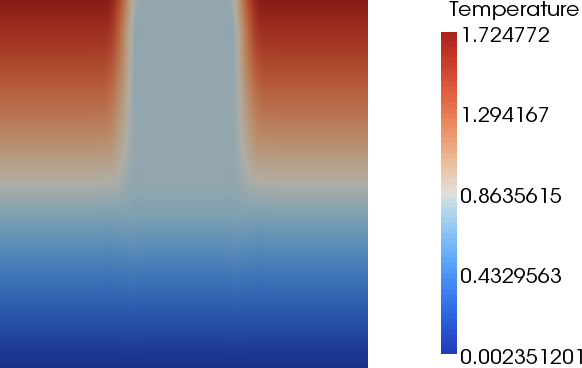
\includegraphics[width=10cm]{examples_images/restratification_after_oodc/rousset-init.png}
\caption{A vertical slice throught the domain showing the initial temperature stratification. The domain is a cylinder of radius 250 km and height 1 km. }
\label{fig:rousset-init}
\end{center}
\end{figure}


The mesh used is a layered mesh, which is created within \fluidity\ from the two dimensional input mesh, \option{circle.geo}. The unstructured triangular mesh is extruded in the vertical, forming triangular prisms which are then divided into unstructured tetrahedra. The columnar arrangement of the nodes is important because the problem has a large aspect ratio, and the elements themselves are wider than they are tall. A fully unstructured mesh would create errors in the pressure, which would then cause errors in the velocity. The layered mesh may be considered to be a special case of the two plus one mesh, in which the nodes are still vertically aligned, but there are different mesh resolutions in different areas of the domain. The resolution is 5 km in the horizontal and 83 m in the vertical. 


A $\PoDGPt$ element pair is used. This means that the discretisation is $P_{1\mathrm{DG}}$ for velocity and  $P2$ continuous for pressure. In this case, the temperature is $P1$ continuous. The benefits of $\PoDGPt$ are discussed in \ref{sec:velocity_pressure_element_pairs}.  To make it more stable, subcycling is switched on under velocity with a maximum Courant number per subcycle of $0.1$. There is a diagnostic free surface field, which requires a free surface boundary condition under the \option{Velocity} options.

The timestep is 7200 s and there are two non-linear iterations.  The timestep is constrained by the Courant condition, but is allowed to be bigger than would otherwise be expected because an absorption field is added under the \option{Velocity} options.  If this field were not added, the time steps would be limited by the scale of the baroclinic waves.  This term has a vertical component equal to  ${\nicefrac{1}{\rho_0}} {\theta} {\Delta} {t} {g} {\frac{\partial \rho}{\partial z}}$ and the other components are zero. $\rho_0$ is the reference density, $\theta$ is the value set under \option{\ldots/Velocity/temporal\_discretisation/theta}, ${\Delta} {t} $ is the timestep, $g$ is the acceleration due to gravity and $\frac{\partial \rho}{\partial z}$ is the background density stratification.   In this case the absorption term is $0.025$ in the vertical and $0.0$ in the horizontal. The \option{\ldots/Absorption/include\_pressure\_correction} option is turned on. 

\subsection{Results}

Figure \ref{fig:rousset-40m} shows the temperature field for a cross section at $40$ m depth at days $10$, $20$, $30$ and $40$. As the column mixes with the surroundings, eddies form at the perimeter of the cylinder. These eddies play a role in the mixing. If this is run with a different resolution, then a different number of eddies may form. The mixing stats diagnostic allows us to quantify the amount of mixing that takes place. It calculates the volume of fluid that has a value of temperature (or other tracer) within certain user-specified bounds as a function of time, and saves this information in the stat file. Figure \ref{fig:rousset-mixing} shows the output from this diagnostic, plotted using the python file provided in the examples directory. The temperature is in units from $0$ to $0.72$. The $0.7$--$0.8$ bin decreases in volume during the course of the simulation because the cold cylinder is mixing with the surrounding stratified fluid.


\begin{figure}[h!]
\begin{center}
\subfigure [10 days]{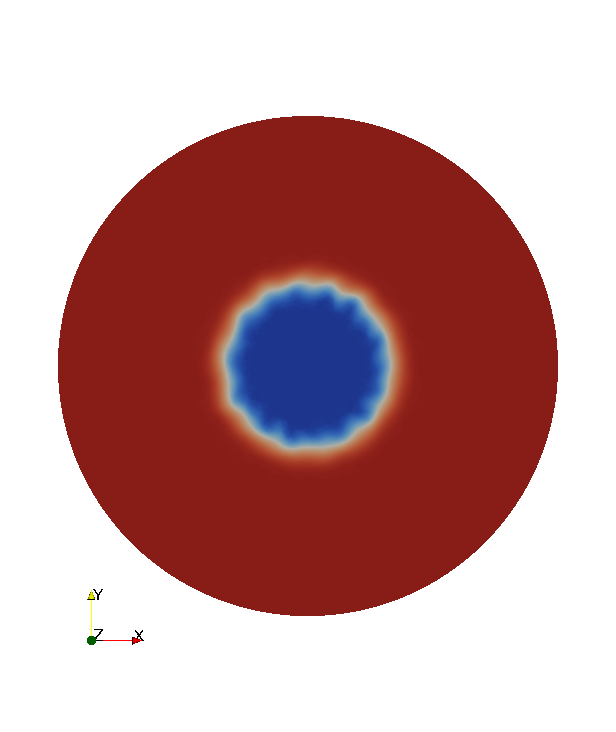
\includegraphics[width=4cm]{examples_images/restratification_after_oodc/5000/rousset-res5000-depth-40m0003.png}}
\hspace{1cm}
\subfigure [20 days]{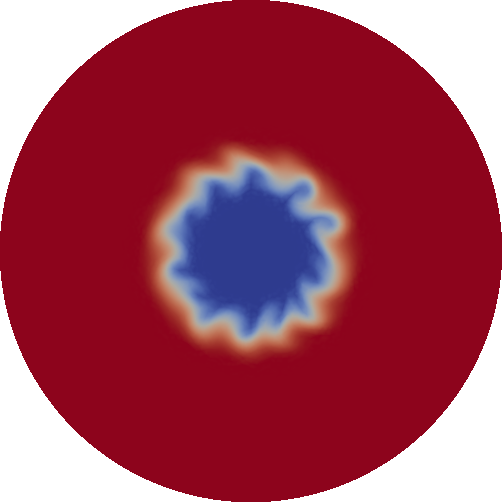
\includegraphics[width=4cm]{examples_images/restratification_after_oodc/5000/rousset-res5000-depth-40m0005.png}}

\subfigure [30 days]{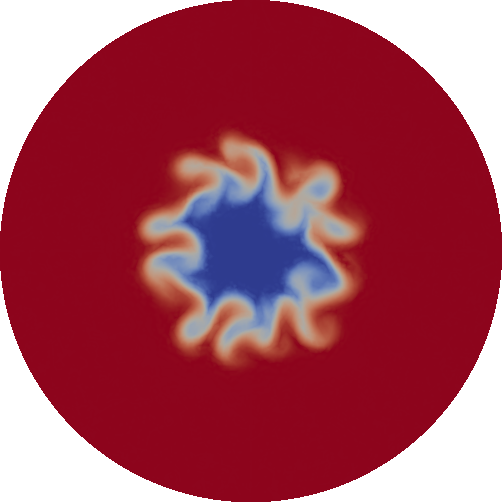
\includegraphics[width=4cm]{examples_images/restratification_after_oodc/5000/rousset-res5000-depth-40m0007.png}}
\hspace{1cm}
\subfigure [40 days]{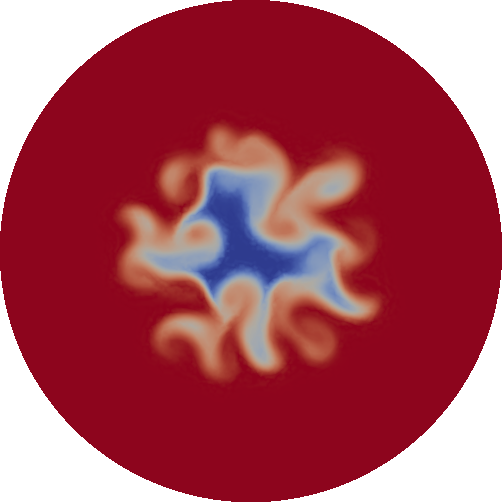
\includegraphics[width=4cm]{examples_images/restratification_after_oodc/5000/rousset-res5000-depth-40m0009.png}}
\caption{The temperature cross-section at a depth of 40m.}
\label{fig:rousset-40m}
\end{center}
\end{figure}


\begin{figure}[h!]
\begin{center}
{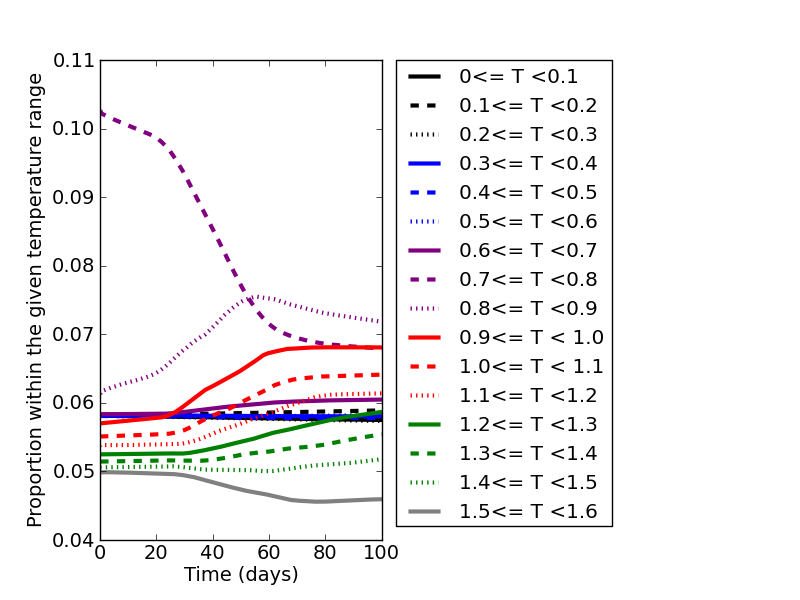
\includegraphics[width=12cm]{examples_images/restratification_after_oodc/mixing_stats.png}}
\caption{Results of the mixing stats diagnostic, showing how the temperature is mixed during the simulation. There is initially most water with a temperature of 0.7-0.8. This mixes during the course of the simulation.}
\label{fig:rousset-mixing}
\end{center}
\end{figure}



%%%%%%%%%%%%%%%%%%%%%%%%%%%%%%%%%%%%%%%%%%%%%%%%%%%%%%%%%%%%%%%%%%%
%---Tides in the Mediterranean Sea--------------------%
%%%%%%%%%%%%%%%%%%%%%%%%%%%%%%%%%%%%%%%%%%%%%%%%%%%%%%%%%%%%%%%%%%%


\section{Tides in the Mediterranean Sea}
\label{sec:tides_in_the_med}

\subsection{Overview}

Tidal modelling is a widely used method for validating free surface implementations \citep{Shum1997}. The Mediterranean Sea
is a good example as it requires both astronomical and co-oscillating boundary tide forcing to obtain
an accurate solution \citep{Tsimplis1995, Wells2008}. An abundance of available tide gauge data recording the 
harmonic constants for both the amplitude and phase of a wide variety of different tidal constituents
facilitates comparisons between ICOM and real-world data. 
 

\subsection{Configuration}

The domain extends from 8$^\circ$W to 40$^\circ$E and from 28$^\circ$N to 48$^\circ$N with an open boundary adjacent to the Atlantic
Ocean in the west. The fixed mesh was generated using gmsh with shoreline data taken from the intermediate resolution $gshhs$
dataset (see \url{http://www.ngdc.noaa.gov/mgg/shorelines/gshhs.html}). The single-element deep tetrahedal elements were then
extruded in the vertical to fit a 3 arc-minute resolution bathymetric profile subsampled from the 1 arc-minute GEBCO dataset     
(see \url{http://www.gebco.net/}). A minimum depth of 3 m  is set to prevent wetting-and-drying related numerical instabilities.

The model is is driven by both astronomical and co-oscillating boundary tide forcing (see sections \ref{astronomical} and \ref{sec:boundary_tide})
for the four main tidal constituents; M$_{\text{2}}$, S$_{\text{2}}$, K$_{\text{1}}$ and O$_{\text{1}}$ (see \citealp{Schwiderski1980,Wells2008}).
Boundary tide data is sourced from the highly accurate FES2004 model \citep{Lyard2006} which is read in from a NetCDF file (see section\ref{sec:BCs:specialised}). 
Frictional drag is applied as a surface-integral boundary condition to the bottom and sides and is based on a quadratic friction law 
of the form $-C_{D}|u|u$, where $C_{D}$ is the drag coefficient, $u$ is the velocity vector 
(ms$^{\text{-1}}$) and $|u|$ is the magnitude of the velocity vector ($|u|=\sqrt{u_{c}^{2}+v_{c}^{2}+w_{c}^{2}}$ where $u_{c}$ is the $x$ component of 
velocity (ms$^{\text{-1}}$), 
$v_{c}$ is the $y$ component of velocity (ms$^{\text{-1}}$) and $w_{c}$ is the 
$z$ component of velocity (ms$^{\text{-1}}$) respectively). 
The $C_{D}$ is set 0.0025, a value considered suitable for the majority of numerical ocean tidal models \citep{Wells2008}. 

The model outputs the harmonic constants for the amplitude and phase of each constituent as calculated from a time series using the least-squares
method. The timestep is 200 entries in length with data recorded every 5 timesteps after an initial spin up period of 20 hours (simulated time). 
The timestep itself is 5 minutes. The total runtime is 200 hours (simulated time).


\subsection{Results}

The harmonic amplitudes are presented as plotted scalar fields and compared with a high-resolution 2D model of \citet{Tsimplis1995} in
Figure \ref{amp}. The model results are similar to those of \citet{Tsimplis1995} and generally predict the correct patterns. 
The semidiurnal constituents give very similar results due to their similar frequencies (Figure \ref{amp}A - D). The amphidromic
systems are correctly located in the Sicilian Channel between Sicily and Libya     
and in the northern Adriatic. The degenerate amphidromes are also accurately positioned near the Balearic Islands and in between
Crete and Libya. The model also captures the amplification of the tidal amplitudes in both the Gulf of gables and the northern Adriatic, 
a phenomena primarily due to resonance of the wave in these regions.

The amplitudes for the diurnal constituents show a similarly good match with the results of \citet{Tsimplis1995} (Figure \ref{amp}E - H).
The lowest amplitudes occur in the eastern part of the basin and there is pronounced amplification in the Adriatic Sea caused by this region
acting as a quarter-wave oscillator with the diurnal frequency \citep{Wells2008}. The degenerate amphidrome
along the Libyan coast (around the Gulf of Sirte) is correctly predicted.   

\begin{figure}[t!]
\centering
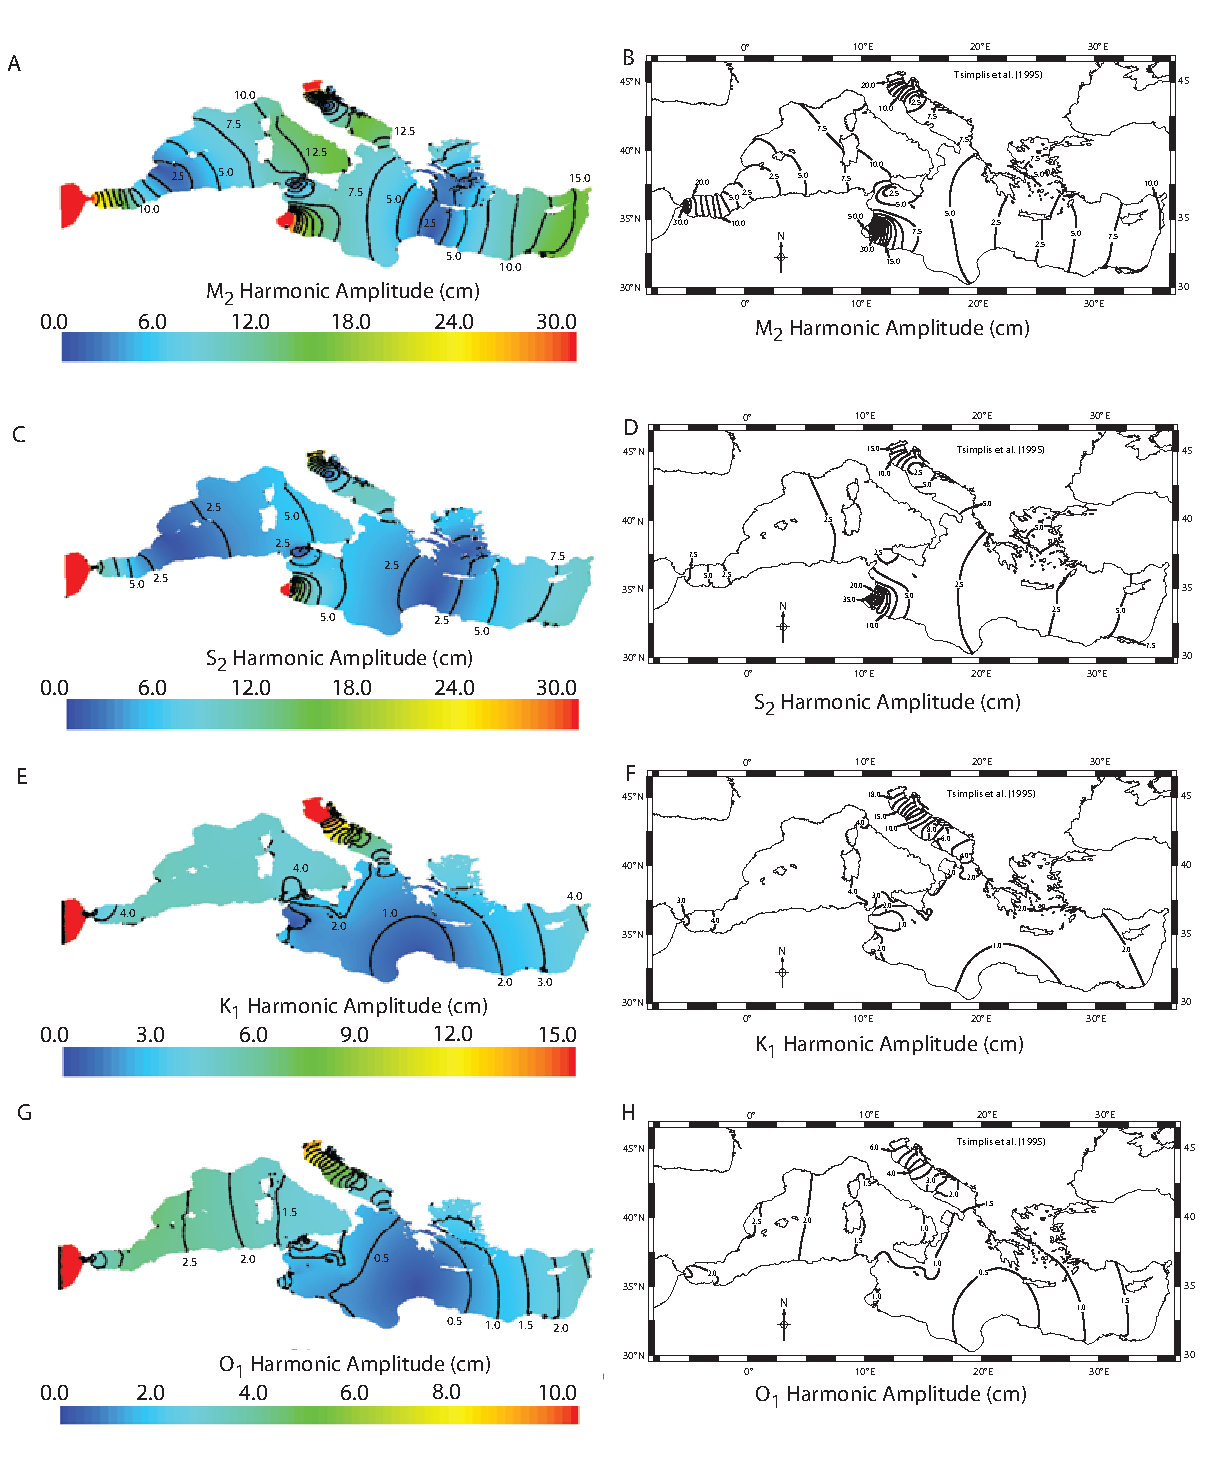
\includegraphics[width=\textwidth]{./examples_images/tides_in_the_Mediterranean_Sea/amp.pdf}
\caption{Plots of the tidal harmonic amplitudes in the Mediterranean Sea from ICOM and the high resolution
model of \citet{Tsimplis1995}.}
\label{amp}
\end{figure}

\begin{figure}[t!]
\centering
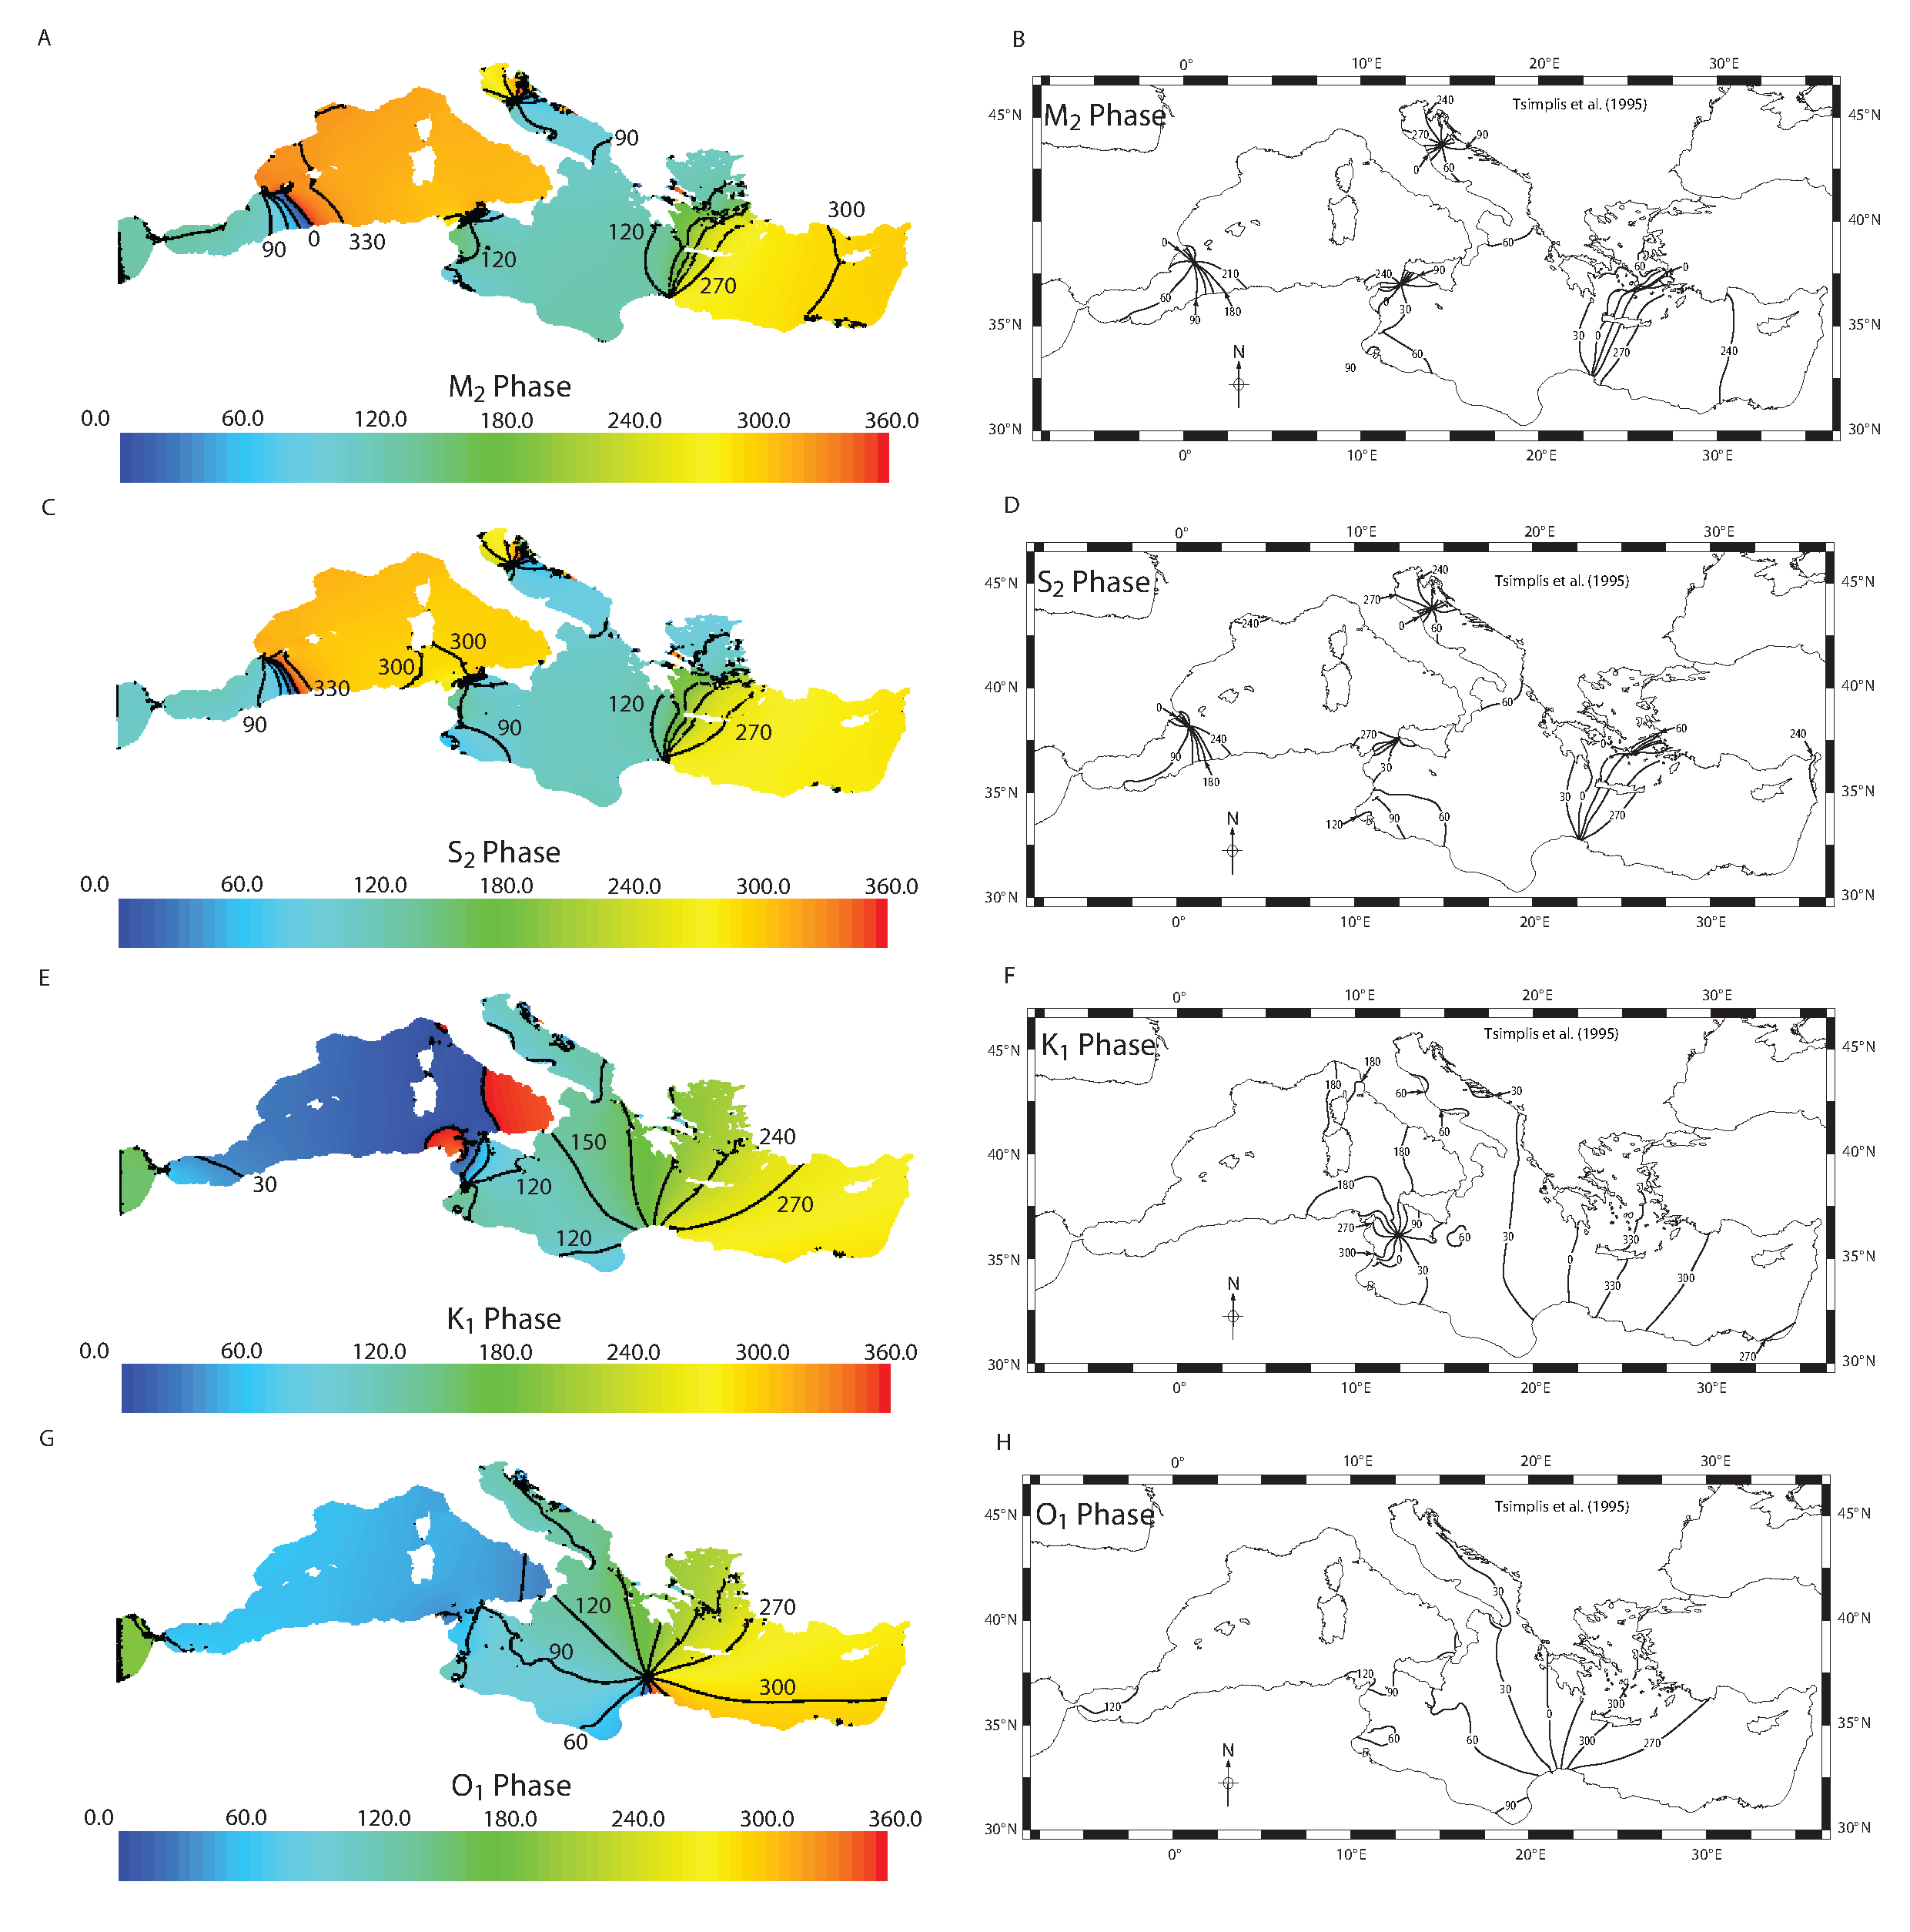
\includegraphics[width=\textwidth]{./examples_images/tides_in_the_Mediterranean_Sea/phase.pdf}
\caption{Plots of the tidal harmonic phases in the Mediterranean Sea from ICOM and the high resolution
model of \citet{Tsimplis1995}. } 
\label{phase}
\end{figure}

The phases as predicted by ICOM and by \citet{Tsimplis1995} are presented in Figure \ref{phase}. These show
a general agreement with the amphidromic systems shown to be rotating in an anti-clockwise direction; a feature
brought about by Coriolis force deflecting the tidal wave to the right in the Northern Hemisphere.
ICOM appears to slightly overpredict the wave speed in all cases; a result that could be attributed to any number of eatures including the
bathymetric/mesh resolution and/or an insufficiently low drag coefficient. Another possible source of error is that the
phase of the boundary tide and the natural mode of oscillation of the basin might not be synchronised; something that
\citet{Tsimplis1995} adjusted repeatedly until they achieved their best results.
 
The harmonic amplitudes are compared with data from 62 tide gauges (Figure \ref{gauge}; \citealp{Tsimplis1995,Wells2008}).
The RMS differences for ICOM are typically 2-3 times those of \citet{Tsimplis1995}    
with the largest errors being for the diurnal constituents (Table \ref{rms}). Despite these discrepancies, the
magnitudes of the RMS differences indicate a good match with the tide gauges, even in a strongly microtidal environment 
such as the Mediterranean Sea. 

\begin{figure}[htbp]
\centering
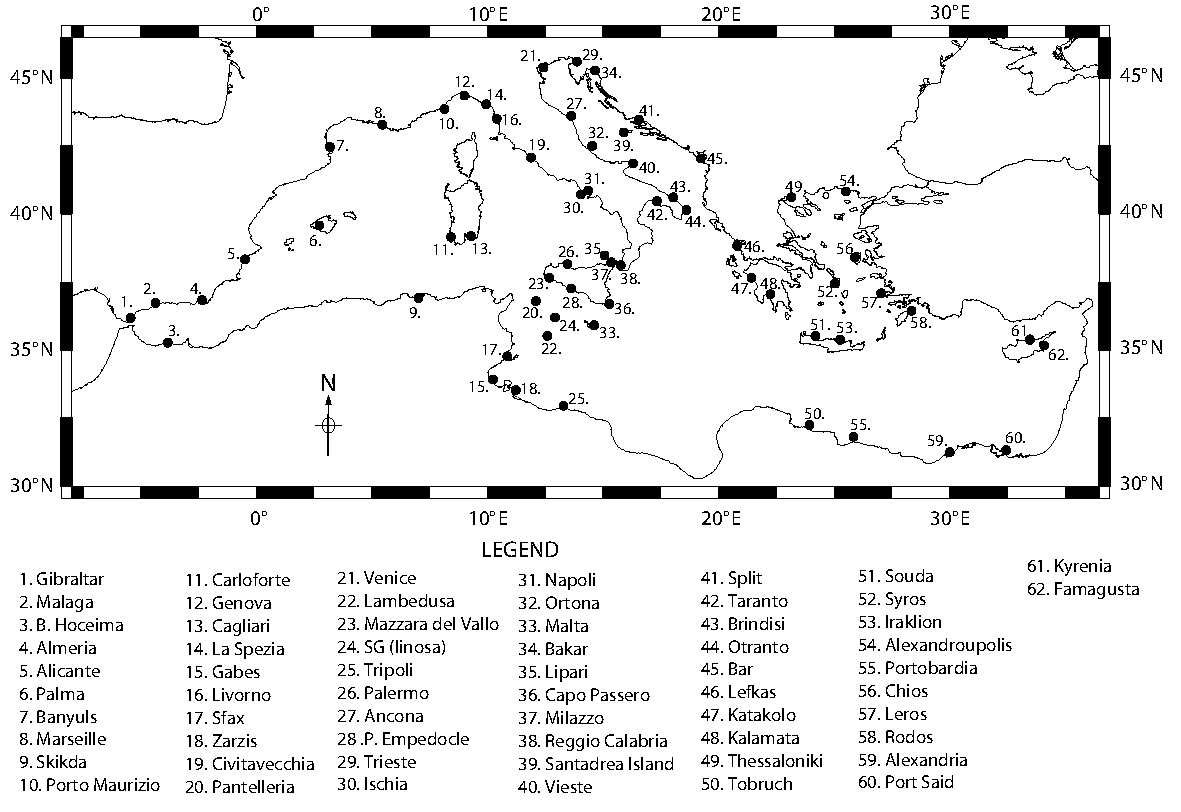
\includegraphics[width=\textwidth]{./examples_images/tides_in_the_Mediterranean_Sea/gauges.pdf}
\caption{Locations of 62 tide gauges in the Mediterranean Sea. Modified from \citet{Wells2008} with data originally taken from 
\citet{Tsimplis1995}. }
\label{gauge}
\end{figure}

\begin{table}[htbp]
\centering
\begin{tabular}{l c c}
\hline
\bf{Tidal Constituent} & \multicolumn{2}{c}{\bf{RMS Differences}} \\
\cline{2-3}
& \bf{\citet{Tsimplis1995}} & \bf{ICOM} \\
\hline
M$_{\text{2}}$ &1.37 & 3.2\\
S$_{\text{2}}$ &0.68 & 1.9\\
K$_{\text{1}}$ &0.82 & 1.7\\
O$_{\text{1}}$ &0.34 & 1.2\\
\hline
\end{tabular}
\caption{RMS differences between modelled harmonic amplitudes and real-world data from 62 tide gauges.
Data is presented from \citet{Tsimplis1995} and ICOM. }
\label{rms}
\end{table}

The quality of the match is further highlighted in scatter diagrams plotting 
the harmonic amplitudes from ICOM at each gauge location against the tide gauge data (Figure \ref{plots}).
These reveal how although ICOM tends to marginally overpredict the amplitude there is a strong
positive correlation closely delineating $y=x$. 

\begin{figure}[t]
\centering
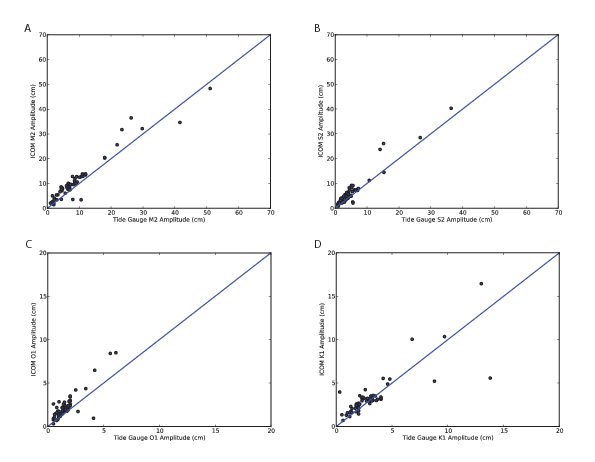
\includegraphics[width=\textwidth]{./examples_images/tides_in_the_Mediterranean_Sea/plots}
\caption{Scatter diagrams plotting harmonic amplitudes from ICOM at each gauge location against tide gauge data.} 
\label{plots}
\end{figure}


%%%%%%%%%%%%%%%%%%%%%%%%%%%%%%%%%%%%%%%%%%%%%%%%%%%%%%%%%%%%%%%%%%%
%---------------------HOKKAIDO-NANSEI-OKI TSUNAMI-----------------%
%%%%%%%%%%%%%%%%%%%%%%%%%%%%%%%%%%%%%%%%%%%%%%%%%%%%%%%%%%%%%%%%%%%

\section{Hokkaido-Nansei-Oki tsunami}
\label{sec:hokkaido-nansei-oki_tsunami}

\subsection{Overview}
This example demonstrates the capabilities of simulating wetting and drying processes in \fluidity.
The event of interest is the Okushiri tsunami in 1993 caused by the Hokkaido Nansei-Oki earthquake offshore of southwestern Hokkaido Island, Japan. 
This earthquake reached a magnitude of 7.8 (Mw) and the resulting tsunami hit a sparsely populated part of the Okushiri island, Japan with a runup height of up to 30m.

To investigate the danger of such events, the Research Institute for Electric Power Industry (CRIEPI) in Abiko, Japan constructed a $1/400$ laboratory model of the area around the island \cite{liu2008advanced}. 
The following configuration simulates this laboratory setup and uses the experimental measurements to benchmark \fluidity.

Fluidity features used in this example:
\begin{itemize}
\item Free surface with wetting and drying, see \ref{subsec:free_surface_bc}.
\item Detectors, see \ref{detectors_options}.
\end{itemize}

\subsection{Configuration}
The simulation configuration resembles the experimental setup as closely as possible. 
The considered domain is a basin with walls on each side except the left where the water level is enforced. 
The basin measures $5.448\mbox{m} \times 3.402\mbox{m}$ and the bathymetry and coastal topography correspond to measurement data, see Figure \ref{fig:monai_inputwave}.
Three surface elevation gauge stations were deployed in the experiment.
Detectors  extract the surface elevation information at every timestep. 
\begin{figure}
\begin{center}
\includegraphics[width=0.7\textwidth]{./examples_images/hokkaido-nansei-oki_tsunami/MonaiValleyDomainWithInputWave2_png.pdf}
\end{center}
\caption{The bathymetry and the three gauge stations used for the Hokkaido-Nansei-Oki tsunami example.}\label{fig:monai_inputwave}
\end{figure}

The mesh used for the simulation is a single layer horizontally unstructured mesh consisting of $19,506$ tetrahedral elements with increased resolution near the inundation areas.
The equations are solved with the $P_1-P_1$ finite element pair, a backward Euler time discretisation with a time-step of $0.1$s.
The wetting and drying algorithm in \fluidity\ requires the user to set a minimal water level thickness, which is here set to $d_0=0.5$mm. If the water surface reaches that level at a point, this point is defined to be dry.
The isotropic kinematic viscosity and gravity magnitude are set to $0.01\mbox{m}^{2}\mbox{s}^{-1}$ and $9.81\mbox{ms}^{-2}$, respectively.
On the left boundary the tsunami wave shown in \ref{fig:monai_inputwave} is prescribed and no-normal flow boundary conditions are applied at the other sides of the domain and the bottom to resemble the solid boundaries in the experiment.
In addition, a Manning-Strickler drag is used at the bottom with $n=0.002\mbox{sm}^{-\frac{1}{3}}$.
To prevent wave breaking in the simulation, this coefficient is increased to $0.2\mbox{sm}^{-\frac{1}{3}}$ in a rectangular area with a side length of $0.5$m centred at $(3.4\mbox{m}, 1.7\mbox{m})$ (which is the centre of the island in the domain) and a fourth order stabilization is applied to prevent wave breaking. 

\subsection{Results}
The result of this example is shown in Figure \ref{fig:monai_results}. 
The plot shows the surface elevation measurements at the three gauge stations of the laboratory experiment compared to the values from the simulation.
\begin{figure}
\begin{center}
\includegraphics[width=0.7\textwidth]{./examples_images/hokkaido-nansei-oki_tsunami/MonaiValley_C_p1p1_nu0_01_kmkstab_drag0_002_butcircularoundisland0_2-crop-crop_final2.pdf}
\caption{The input wave elevation of the Okushiri tsunami test case (a) and the numerical and experimental results at ``Gauge 1'' (top), ``Gauge 2'' (middle) and ``Gauge 3'' (bottom) (b).}\label{fig:monai_results}
\end{center}
\end{figure}

\subsection{Exercises}
\begin{enumerate}
\item Add more detectors to the simulation.
\item Increase the wetting and drying threshold parameter. Which effects does it have to the result?
\item Change the viscosity parameter. Does it make a difference to the inundation of the tsunami event?
\end{enumerate}


%%%%%%%%%%%%%%%%%%%%%%%%%%%%%%%%%%%%%%%%%%%%%%%%%%%%%%%%%%%%%%%%%%%%%%%%%
%%%%%%%%%%%%%%%%%%%%%%%%%% Tephra settling %%%%%%%%%%%%%%%%%%%%%%%%%%%%%%
%%%%%%%%%%%%%%%%%%%%%%%%%%%%%%%%%%%%%%%%%%%%%%%%%%%%%%%%%%%%%%%%%%%%%%%%%

\section{Tephra settling}
\label{sec:tephra_settling}

\subsection{Overview}
In this example, \fluidity\ is used to replicate a laboratory experiment of tephra (fine volcanic ash particles) settling through a tank of water \citep{carey1997}. The \cite{carey1997} experiments introduced tephra particles into a $0.3\times 0.3\times 0.7$ m tank, filled with water, from above using a delivery system and a particle disperser. The particles settled through the air in the tank at an approximately constant rate until they landed in the water and began to settle through the water at a much reduced velocity. While the particles in the water were sufficiently dispersed their settling velocity was that predicted by Stokes' flow (a few mm/s).  However, the build-up of particles caused by the air-water interface eventually created a layer of particles and water with a bulk density so great, relative to the density of the particle-poor water beneath, as to be gravitationally unstable and promote the formation of a vertical gravity current (plumes). The settling velocity of these plumes of particles and water was observed to be an order of magnitude greater than the Stokes settling velocity of the individual particles.

In the \fluidity\ simulations, rather than represent each tephra particle individually using a multimaterial approach (which would be prohibitively expensive), a ``dispersed multiphase'' approach is adopted (see \ref{sec:multiphase_equations}), in which one phase represents the water in the tank and the other phase represents all the particles dispersed within the water. Similar to the water column collapse example (\ref{sec:water_collapse}), a volume fraction field is used to distinguish between the continuous phase (water) and the dispersed phase (particles). In an element the volume fraction of particles represents the fraction of the element volume that is occupied by particles, which is typically very small. In contrast to the multimaterial approach, however, the multiphase approach assigns each phase a separate velocity, allowing the dispersed phase (particles) to move through the continuous phase (water). In this example, the dispersed phase is more dense than the continuous phase and so sinks under the influence of gravity.

The simulation replicates one of the \cite{carey1997} experiments (with a characteristic particle size of 48 $\mu$m) by considering a constant influx of the particle phase into a 2D tank of water. The simulation results can be compared to the experiment in terms of the conditions under which plumes of tephra particles form as well as the settling velocities of the individual particles and plumes. The example demonstrates the following functionality:
\begin{itemize}
\item 2D flow
\item Multi-phase flow
\item Incompressible flow
\item Adaptive timestepping
\end{itemize}

The simulation illustrated here took $\sim$1 hour to run in serial on an Intel Xeon E5430 2.66 GHz processor.

\subsection{Problem specification}
The simulation uses a 0.3 x 0.7 metre domain, replicating the cross-section of the water tank used in the experiments, with an initial characteristic element size of 0.01 metres. No normal flow boundary conditions are weakly imposed along with a zero velocity initial condition. The parameters for density, viscosity, particle diameter and gravity are $\rho_p = 2340\ \mathrm{kgm^{-3}}$, $\rho_l = 1000\ \mathrm{kgm^{-3}}$, $\mu_l = 0.001\ \mathrm{Pa\cdot s}$, $d = 48\times 10^{-6}\ \mathrm{m}$, and $\mathbf{g} = 9.8\ \mathrm{ms^{-2}}$ respectively (with the subscripts $p$ and $l$ denoting the properties of the particle/tephra and liquid phase).

The influx of particles from the air above is simulated using a \option{flux} boundary condition at the top of the domain. This allows tephra to flux in at a rate of $0.472\ \mathrm{gm^{-2}s^{-1}}$. The results of the experiments showed that tephra particles initially settled individually at a Stokes velocity of $0.17\ \mathrm{cms^{-1}}$. When the concentration was high enough, plumes formed and descended to the bottom of the tank with velocities more than ten times greater than those of individual particles.

\subsection{Results}
Several timesteps of the example simulation can be seen in Figure \ref{fig:tephra_settling_coarse}. These images can be generated by visualising the vtu files using Paraview. Better resolved plumes can be produced by using a smaller characteristic element size (e.g. $\Delta x = 0.0025\ \mathrm{m}$, shown in Figure \ref{fig:tephra_settling_fine}).

\begin{figure}[H]
	\centering
	      
\includegraphics[width=0.19\columnwidth]{./examples_images/tephra_settling/tephra_coarse_1.png}
	      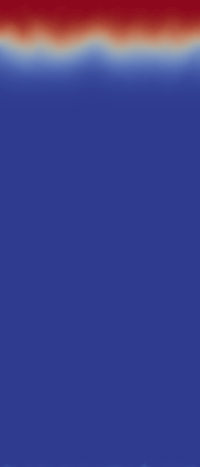
\includegraphics[width=0.19\columnwidth]{./examples_images/tephra_settling/tephra_coarse_2.png}
	      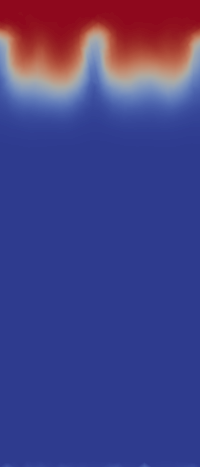
\includegraphics[width=0.19\columnwidth]{./examples_images/tephra_settling/tephra_coarse_3.png}
	      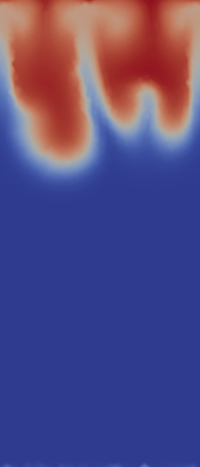
\includegraphics[width=0.19\columnwidth]{./examples_images/tephra_settling/tephra_coarse_4.png}
	      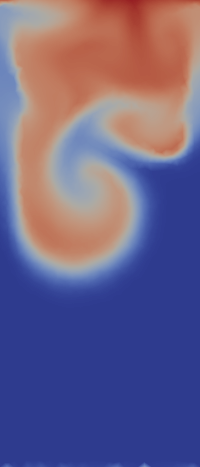
\includegraphics[width=0.19\columnwidth]{./examples_images/tephra_settling/tephra_coarse_5.png}
   \caption{Tephra (particle) phase volume fraction at time $t = 10, 30, 50, 80, 110$ seconds. These images are from a lower-resolution version of the tephra settling example problem, with a characteristic element size of $\Delta x = 0.01\ \mathrm{m}$.}
   \label{fig:tephra_settling_coarse}
\end{figure}

\begin{figure}[H]
	\centering
	      
\includegraphics[width=0.19\columnwidth]{./examples_images/tephra_settling/tephra_fine_1.png}
	      \includegraphics[width=0.19\columnwidth]{./examples_images/tephra_settling/tephra_fine_2.png}
	      \includegraphics[width=0.19\columnwidth]{./examples_images/tephra_settling/tephra_fine_3.png}
	      \includegraphics[width=0.19\columnwidth]{./examples_images/tephra_settling/tephra_fine_4.png}
	      \includegraphics[width=0.19\columnwidth]{./examples_images/tephra_settling/tephra_fine_5.png}
   \caption{Tephra (particle) phase volume fraction at time $t = 10, 30, 50, 80, 110$ seconds. The onset of plumes is between 10 and 30 seconds. Note that these images are from a high-resolution version of the tephra settling example problem, with a characteristic element size of $\Delta x = 0.0025\ \mathrm{m}$.}
   \label{fig:tephra_settling_fine}
\end{figure}

Figure \ref{fig:tephra_settling_velocity} (reproducible by typing \textit{make postprocess} at the command line) illustrates how the tephra particles initially settle at approximately $0.17\ \mathrm{cms^{-1}}$, as predicted by Stokes' law. As more tephra fluxes in, the layer becomes unstable and plumes begin to form, resulting in settling velocities over 10 times greater than that of an individual particle.

\begin{figure}[H]
	\centering
	      \includegraphics[width=0.8\columnwidth]{./examples_images/tephra_settling/tephra_velocity.pdf}
   \caption{Maximum velocity of the tephra phase against time.}
   \label{fig:tephra_settling_velocity}
\end{figure}

\subsection{Exercises}
To explore the multiphase functionality of \fluidity, the following variations on this example would be constructive learning exercises:

\begin{itemize}
\item Decrease the characteristic element size to better resolve the plume behaviour
\item Alter the particle size to observe its affect on plume formation
\item Add a second dispersed phase (with a different particle size).
\end{itemize}

%%%%%%%%%%%%%%%%%%%%%%%%%%%%%%%%%%%%%%%%%%%%%%%%%%%%%%%%%%%%%%%%%%%%%%%%%
%%%%%%%%%%%%%%%%%%%%%%%%%% Stokes square convection  %%%%%%%%%%%%%%%%%%%%
%%%%%%%%%%%%%%%%%%%%%%%%%%%%%%%%%%%%%%%%%%%%%%%%%%%%%%%%%%%%%%%%%%%%%%%%%

\section{Stokes Square Convection}
\label{sec:stokes_square_convection}

\subsection{Overview}

In this example we compare the numerical predictions of \fluidity{} with a well--established two--dimensional cartesian geometry benchmark result for Stokes flow \citep{blankenbach1989}. Fluidity's results from this, and similar cases, are published in \citet{Davies2011}, where solution strategies employed for solving the Stokes system are also discussed. 


\subsection{Problem Specification}

The specific example considered is steady--state isoviscous convection at a Rayleigh number ($Ra$) of $10^{5}$, in a two--dimensional square domain of unit dimensions. Boundary conditions for temperature are $T=0$ at the surface, $T=1$ at the base, with insulating (homogeneous Neumann) side--walls. For velocity, free--slip and no normal flow boundary conditions are specified at all boundaries. 

The example incorporates two cases, on uniform, structured meshes, where the domain is subdivided into $24 \times 24$ and $48 \times 48$ elements, respectively (excluding mesh resolution, each case is identical). For direct comparison with the benchmark solutions, we calculate the Nusselt Number ($Nu$) and RMS velocity ($V_{RMS}$), once a steady--state has been achieved (the variation in the infinity--norm of the velocity and temperature fields is $< 5 \times 10^{-5}$, between consecutive time--steps). The Nusselt Number is defined as:

\begin{equation}
Nu = -z_{\max}\frac{\int_{z=z_{\max}} \sum_{i} n_{i} \partial_{i} T}{\int_{z=0} T},
\end{equation}

\medskip \noindent where $T$ is temperature, $z_{\max}$ is the maximum $z$ coordinate of the domain, $\int_{z=z_{\max}}$ denotes the integral over the top surface of the domain and $\int_{z=0}$ denotes the integral over the bottom surface of the domain.  The RMS velocity is given by:

\begin{equation}
V_{RMS} = \sqrt{\frac{1}{V}{\int \sum_i u_{i}^{2}}}.
\end{equation}

\medskip \noindent Here, $u_{i}$ is the velocity vector, whilst $V$ denotes the domain volume. 

\begin{figure}[t]
	\centering
	      \includegraphics[width=0.90\columnwidth]{./examples_images/stokes_square_convection/Temperature_planform.png}
   \caption{Steady--state temperature field from an isoviscous Stokes simulation at $Ra = 1 \times 10^{5}$, on a uniform structured mesh of $48 \times 48$ elements. Contours are spaced at intervals of 0.1.}
   \label{fig:stokes_square_convection_planform}
\end{figure}

\subsection{Results}

Results are presented in Figures \ref{fig:stokes_square_convection_planform} and \ref{fig:stokes_square_convection_graphs}. The final steady--state solution consists of one convective cell, with hot upwelling flow confined to the left hand side of the domain and cold downwelling flow on the right hand side. Note that, excluding the location of upwelling flow at $x=0$ or $x=1$, results are insensitive to the initial condition. Quantitatively, results show excellent agreement with the benchmark predictions of \citet{blankenbach1989}, with solution accuracy improving with increased resolution, as expected. A higher resolution case (at a resolution of $96 \times 96$ elements), achieves results that are almost identical to the benchmark solution.

\begin{figure}[t]
	\centering
	      \includegraphics[width=0.48\columnwidth]{./examples_images/stokes_square_convection/Nu_1e5.png}
	      \includegraphics[width=0.48\columnwidth]{./examples_images/stokes_square_convection/RMS_1e5.png}
   \caption{Results from 2-D, isoviscous Stokes square convection benchmark cases: (a) Nusselt number vs. number of triangle vertices, at $Ra = 1 \times 10^{5}$ \citep[case 1b:][]{blankenbach1989}, for a series of uniform, structured meshes. Filled circles reporesent the example cases at a resolution of $24 \times 24$ and $48 \times 48$ elements respectively. The open circle represents the result from a case at $96 \times 96$ elements, to illustrate that as mesh resolution is increased, solutions converge towards the benchmark values; (b) RMS velocity vs. number of triangle vertices, at $Ra = 1 \times 10^{5}$. Benchmark values are denoted by horizontal dashed lines. Note that the highest resolution case is not included in the example.}
   \label{fig:stokes_square_convection_graphs}
\end{figure}


\subsection{Exercises}
To explore the Stokes functionality of \fluidity, the following variations on this example would be constructive learning exercises:
\begin{itemize}
\item Verify that results do indeed converge towards the benchmark values at higher resolution.
\item Alter the initial condition for temperature to verify that, excluding the location of upwelling flow at $x=0$ or $x=1$, results are insensitive to this initial condition. 
\item Change the Rayleigh number to $Ra = 1 \times 10^{4}$ and compare your results to Case 1b from \citet{blankenbach1989}.
\end{itemize}

%%%%%%%%%%%%%%%%%%%%%%%%%%%%%%%%%%%%%%%%%%%%%%%%%%%%%%%%%%%%%%%%%%%%%%%%%
